\documentclass[9pt,preprint]{sigplanconf}
\usepackage{amsmath,tabu}
\usepackage{cancel}
\usepackage{amssymb} 
\usepackage{amsthm}
\usepackage{graphicx}
\usepackage[usenames,dvipsnames,svgnames,table]{xcolor}
\newcommand{\copyleft}{\reflectbox{\sffamily\copyright}}
\usepackage{ stmaryrd }
\usepackage{mathpartir}
%\usepackage{cite}
%\renewcommand{\citepunct}{,\,} % IEEEtran wants to use ],\,[ for this but that looks dumb...
\newcommand{\atlam}{@$\lambda$}

% Generic
\newcommand{\bindin}[2]{#1;~#2}
\newcommand{\pipe}{~\text{\large $\vert$}~}
\newcommand{\splat}[3]{#1_{#2};\ldots;#1_{#3}}
\newcommand{\splatC}[3]{#1_{#2}~~~~\cdots~~~~#1_{#3}}
\newcommand{\splatTwo}[4]{#1_{#3}#2_{#3},~\ldots~, #1_{#4}#2_{#4}}
\newcommand{\substn}[2]{[#1]#2}
\newcommand{\subst}[3]{\substn{#1/#2}{#3}}
\newcommand{\entails}[2]{#1 \vdash #2}

% Programs
\newcommand{\progsort}{\rho}
\newcommand{\pfam}[2]{\bindin{#1}{#2}}
\newcommand{\pdef}[4]{\bindin{{\sf def}~\tvar{#1}:#2=#3}{#4}}

% Families
\newcommand{\fvar}[1]{\textsc{#1}}

\newcommand{\family}[6]{{\sf family}~\fvar{#1}[#2]\sim \tvar{#5}.#6~\{#3\}}
\newcommand{\familyDf}{\family{Fam}{\kappaidx}{\opsort}{\opsigsort}{i}{\taurep}}

% Operators
\newcommand{\opsort}{\theta}
\newcommand{\opsigsort}{\Theta}
\newcommand{\opvar}[1]{\textbf{\textit{#1}}}

% Expressions
\newcommand{\evar}[1]{#1}
\newcommand{\elam}[3]{\lambda #1{:}#2.#3}
\newcommand{\eapp}[2]{{#1~#2}}
\newcommand{\eopapp}[2]{\eop{Arrow}{ap}{\tunit}{#1; #2}}
\newcommand{\eop}[4]{{\fvar{#1}.\opvar{#2}\langle#3\rangle(#4)}}
\newcommand{\elet}[4]{{\sf let}~#1 : #2 = #3~{\sf in}~#4}

% Type-Level Terms
\newcommand{\tvar}[1]{{\textbf{#1}}}

\newcommand{\tlam}[3]{\lambda \tvar{#1}{:}{#2}.#3}
\newcommand{\tapp}[2]{#1~#2}
\newcommand{\tifeq}[5]{{\sf if}~#1\equiv_{#3}#2{\sf ~then~}#4~{\sf else}~#5}
\newcommand{\tstr}[1]{\textit{``#1''}}
\newcommand{\tunit}{()}
\newcommand{\tpair}[2]{(#1, #2)}
\newcommand{\tfst}[1]{{\sf fst}(#1)}
\newcommand{\tsnd}[1]{{\sf snd}(#1)}
\newcommand{\tnil}[1]{[]_#1}
\newcommand{\tcons}[2]{#1 :: #2}
\newcommand{\tfold}[6]{{\sf fold}(#1; #2; \tvar{#3},\tvar{#4},\tvar{#5}.#6)}

\newcommand{\tfamSpec}[5]{{\sf family}~[#2]~::~#3~\{#4 : #5\}}
\newcommand{\tfamSpecStd}{\tfamSpec{fam}{\kappaidx}{\taurep}{\theta}{\Theta}}

\newcommand{\ttype}[2]{\fvar{#1}\langle#2\rangle}
\newcommand{\ttypestd}{\ttype{Fam}{\tau}}
\newcommand{\tfamcase}[5]{{\sf case}~#1~{\sf of}~\fvar{#2}\langle\tvar{#3}\rangle\Rightarrow#4~{\sf ow}~#5}
\newcommand{\trepof}[1]{{\sf rep}(#1)}

\newcommand{\tden}[2]{\llbracket #1~{\sf as}~#2 \rrbracket}
\newcommand{\ttypeof}[1]{{\sf typeof}~#1}
\newcommand{\tvalof}[2]{{\sf trans}(\tden{#1}{#2})}
\newcommand{\terr}{{\sf err}}
\newcommand{\tdencase}[5]{{\sf case}~#1~{\sf of}~\tden{\tvar{#2}}{\tvar{#3}}\Rightarrow#4~{\sf ow}~#5}

\newcommand{\titerm}[1]{\triangledown(#1)}
\newcommand{\titype}[1]{\blacktriangledown(#1)}

\newcommand{\tconst}[1]{{\sf const}(#1)}
\newcommand{\tOp}[1]{{\sf op}(#1)}

\newcommand{\tprog}[1]{{\sf program}(#1)}

\newcommand{\topsempty}{\cdot}
\newcommand{\tops}[5]{\opvar{#1}[#2](\tvar{#3},\tvar{#4}.#5)}
\newcommand{\topp}[2]{#1; #2}
\newcommand{\Tops}[2]{\tvar{#1} : #2}
\newcommand{\Topp}[2]{#1; #2}
\newcommand{\kOpEmpty}{\cdot}
\newcommand{\kOpS}[2]{\opvar{#1}[#2]}
\newcommand{\kOp}[3]{#1; \kOpS{#2}{#3}}

% Contexts
\newcommand{\fCtx}{\Sigma}
\newcommand{\itvarCtx}{\Omega}
\newcommand{\iCtx}{\Theta}
\newcommand{\eCtx}{\Gamma}
\newcommand{\etvarCtx}{\Omega}
\newcommand{\errCtx}{\mathcal{E}}
\newcommand{\famEvalCtx}{\Xi}

% Judgments
\newcommand{\emptyctx}{\emptyset}
\newcommand{\tvarCtx}{\Delta}
\newcommand{\tvarCtxX}[2]{\Delta, {\tvar{#1}} : {#2}}
\newcommand{\fvarCtx}{\Sigma}
\newcommand{\fvarCtxX}{\Sigma, \fvarOfType{Fam}{\kappaidx}{\Theta}}
\newcommand{\eivarCtx}{\Omega}
\newcommand{\eivarCtxX}[1]{\Omega, \evar{#1}}

\newcommand{\kEntails}[3]{#1 \vdash_{#2} #3}

\newcommand{\progProg}[1]{#1~{\tt prog}}
\newcommand{\progOK}[3]{\kEntails{#1}{#2}{\progProg{#3}}}
\newcommand{\progOKX}[1]{\progOK{\tvarCtx}{\fvarCtx}{#1}}

\newcommand{\fvarOfType}[3]{\fvar{#1}[#2,#3]}
\newcommand{\fvarOfTypeDf}{\fvarOfType{Fam}{\kappaidx}{\Theta}}

\newcommand{\opOfType}[2]{#1 : #2}
\newcommand{\opType}[4]{\kEntails{#1}{#2}{\opOfType{#3}{#4}}}

\newcommand{\tOfKind}[2]{#1 : #2}
\newcommand{\tKind}[4]{\kEntails{#1}{#2}{\tOfKind{#3}{#4}}}
\newcommand{\tKindX}[2]{\tKind{\tvarCtx}{\fvarCtx}{#1}{#2}}

\newcommand{\isExpr}[1]{#1~\texttt{expr}}
\newcommand{\exprOK}[4]{#1~#2 \vdash_{#3} \isExpr{#4}}
\newcommand{\exprOKX}[1]{\exprOK{\tvarCtx}{\eivarCtx}{\fvarCtx}{#1}}

\newcommand{\isIterm}[4]{#1~#2 \vdash_{#3} #4~\texttt{iterm}}
\newcommand{\isItermX}[1]{\isIterm{\tvarCtx}{\eivarCtx}{\fvarCtx}{#1}}

\newcommand{\isItype}[3]{#1 \vdash_{#2} #3~\texttt{itype}}
\newcommand{\isItypeX}[1]{\isItype{\tvarCtx}{\fvarCtx}{#1}}

\newcommand{\tEvalX}[2]{#1 \Downarrow #2}
\newcommand{\tiEvalX}[2]{#1 \curlyveedownarrow #2}

\newcommand{\fvalCtx}{\Phi}
\newcommand{\fvalCtxX}[1]{\Phi, #1}
\newcommand{\fval}[4]{\fvar{#1}[#2, \tvar{#3}.#4]}
\newcommand{\fvalDf}{\fval{Fam}{\theta}{i}{\tau}}

\newcommand{\pcompiles}[3]{\vdash_{#1} #2 \Longrightarrow #3}
\newcommand{\pcompilesX}[1]{\pcompiles{\fvalCtx}{#1}{\gamma}}

\newcommand{\ptcc}[2]{#1 \longrightarrow #2}

\newcommand{\etCtx}{\Gamma}
\newcommand{\etCtxX}[2]{\etCtx, \evar{#1} : #2}

\newcommand{\gtCtx}{\Psi}
\newcommand{\gtCtxX}[2]{\gtCtx, \evar{#1} : #2}

\newcommand{\ecompiles}[5]{#1 \vdash_{#2} #3 : #4 \Longrightarrow #5}
\newcommand{\ecompilesX}[3]{\ecompiles{\etCtx}{\fvalCtx}{#1}{#2}{#3}}

\newcommand{\delfromtau}[4]{\vdash^{\fvar{#1}}_{#2} #3 \sim #4}
\newcommand{\tauisdel}[5]{\vdash^{\fvar{#1}}_{#2} \ttype{#3}{#4} \sim #5}

\newcommand{\checkRC}[5]{#1 \vdash^{\fvar{#2}}_{#3} #4 \sim #5}
\newcommand{\checkRCX}[2]{\checkRC{\gtCtx}{Fam}{\fvalCtx}{#1}{#2}}

\newcommand{\erase}[3]{\vdash_{#1} #2 \leadsto #3}
\newcommand{\eraseX}[2]{\erase{\fvalCtx}{#1}{#2}}

\newcommand{\eCtxTogCtx}[4]{\vdash^{\fvar{#1}}_{#2} #3 \sim #4}
\newcommand{\eCtxTogCtxX}[2]{\eCtxTogCtx{Fam}{\fvalCtx}{#1}{#2}}

\newcommand{\ddbar}[4]{\vdash^{\fvar{#1}}_{#2} #3 \sim #4}
\newcommand{\ddbarX}[2]{\ddbar{Fam}{\fvalCtx}{#1}{#2}}

\newcommand{\iType}[3]{#1 \vdash #2 : #3}

\newcommand{\gtCtxH}{\hat{\gtCtx}}
\newcommand{\gtCtxHX}[2]{\gtCtxH, \evar{#1} : #2}

%
\newcommand{\fSpec}[3]{\tof{\fvar{#1}}{\kFam{#2}{#3}}}
\newcommand{\fSpecStd}{\fSpec{fam}{\kappaidx}{\Theta}}

% \tau
\newcommand{\taut}[1]{{\tau_{\text{#1}}}}
\newcommand{\tautype}{\taut{type}}
\newcommand{\tautrans}{\taut{trans}}
\newcommand{\tauproof}{\taut{proof}}
\newcommand{\tauidx}{\taut{idx}}
\newcommand{\taui}{\taut{i}}
\newcommand{\tauidxn}[1]{\taut{idx,#1}}
\newcommand{\taurep}{\taut{rep}}
\newcommand{\taurepn}[1]{\taut{rep,#1}}
\newcommand{\tauden}{\taut{den}}
\newcommand{\tauIT}{\taut{IT}}
\newcommand{\tauarrow}{\taut{arrow}}
\newcommand{\tauprod}{\taut{prod}}
\newcommand{\tauint}{\taut{int}}
\newcommand{\taubool}{\taut{bool}}
\newcommand{\tauprog}{\taut{prog}}
\newcommand{\tauiterm}{\taut{iterm}}
\newcommand{\tauval}{\taut{val}}
\newcommand{\tauop}{\taut{op}}

% \gamma
\newcommand{\ghat}{\hat{\gamma}}

% \sigma
\newcommand{\delt}[1]{\sigma_{\text{#1}}}
\newcommand{\delrep}{\delt{rep}}
\newcommand{\dhat}{\hat{\sigma}}
\newcommand{\dbar}{\bar{\sigma}}

% \kappa
\newcommand{\kappat}[1]{\kappa_{\text{#1}}}
\newcommand{\kappaidx}{\kappat{idx}}
\newcommand{\kappai}{\kappat{i}}

% Types

% IL terms
\newcommand{\ivar}[1]{\textrm{#1}}
\newcommand{\ilam}[3]{\lambda #1{:}#2.#3}
\newcommand{\ifix}[3]{{\sf fix~}#1{:}#2~{\sf is}~#3}
\newcommand{\iapp}[2]{#1~#2}
\newcommand{\ipair}[2]{(#1, #2)}
\newcommand{\ifst}[1]{{\sf fst}(#1)}
\newcommand{\isnd}[1]{{\sf snd}(#1)}
\newcommand{\iintlit}{\bar{
\textrm{z}}}
\newcommand{\iop}[2]{#1 \oplus #2}
\newcommand{\iIfEq}[5]{{\sf if}~#1\equiv_{#3}#2{\sf ~then~}#4~{\sf else}~#5}
\newcommand{\mvalof}[1]{{\sf valof}(#1)}
\newcommand{\iup}[1]{\vartriangle\hspace{-2.5pt}(#1)}

% Internal Types
\newcommand{\darrow}[2]{#1\rightarrow#2}
\newcommand{\dint}{\mathbb{Z}}
\newcommand{\dpair}[2]{#1\times#2}
\newcommand{\dup}[1]{\blacktriangle(#1)}
\newcommand{\drepof}[1]{{\sf repof}(#1)}

% Kinds
\newcommand{\kvar}[1]{\textrm{#1}}
\newcommand{\karrow}[2]{#1\rightarrow{#2}}
\newcommand{\kforall}[2]{\forall \kvar{#1}.#2}
\newcommand{\kstr}{\textsf{Str}}
\newcommand{\kunit}{\textsf{1}}
\newcommand{\kpair}[2]{#1 \times #2}
\newcommand{\klist}[1]{\textsf{list}[#1]}
\newcommand{\kTypeBlur}{\star}
\newcommand{\kDen}{\textsf{Den}}
\newcommand{\kIType}{\textsf{ITy}}
\newcommand{\kITerm}{\textsf{ITm}}

% Judgements
\newcommand{\tof}[2]{#1 : #2}
\newcommand{\mtof}[2]{#1 :: #2}
\newcommand{\tentails}[2]{#1 \vdash #2}
\newcommand{\tentailst}[3]{\tentails{#1}{\tof{#2}{#3}}}
\newcommand{\tStdCtx}{\fCtx~\tvarCtx}
\newcommand{\tCtxXF}[1]{\fCtx, #1~\tvarCtx}
\newcommand{\tCtxXT}[1]{\fCtx~\tvarCtx, #1}
%\newcommand{\tCtxXL}[1]{\fCtx~\tvarCtx~\lvarCtx, #1}
\newcommand{\tentailsX}[1]{\tentails{\tStdCtx}{#1}}
\newcommand{\tentailsXt}[2]{\tentailsX{\tof{#1}{#2}}}
\newcommand{\kentails}[2]{#1 \vdash #2}
\newcommand{\kentailsX}[1]{\kentails{\fCtx}{#1}}
\newcommand{\iMkCtx}[3]{#1~#2~#3}
\newcommand{\iStdCtx}{\iMkCtx{\fCtx}{\tvarCtx}{\itvarCtx}}
\newcommand{\ientails}[2]{#1 \vdash #2}
\newcommand{\ientailsX}[1]{\entails{\iStdCtx}{#1}}
\newcommand{\casemap}[2]{#1 : #2}
\newcommand{\mentails}[3]{#1, #2 \vdash #3}
\newcommand{\mentailsX}[1]{\mentails{\tvarCtx}{\itvarCtx}{#1}}
\newcommand{\eentails}[4]{#1~#2~#3 \vdash #4}
\newcommand{\eentailsX}[1]{\eentails{\fCtx}{\tvarCtx}{\etvarCtx}{#1}}
\newcommand{\mtentails}[2]{#1 \vdash #2}
\newcommand{\mtentailsX}[1]{\mtentails{\iCtx}{#1}}
\newcommand{\mtentailsXt}[2]{\mtentails{\iCtx}{\mtof{#1}{#2}}}
\newcommand{\kSimple}[1]{#1~{\sf simple}}
\newcommand{\Tentails}[3]{#1 \vdash_{#2} #3}
\newcommand{\TentailsX}[1]{\Tentails{\fCtx}{\fvar{fam}}{#1}}
\newcommand{\kEq}[1]{#1~\texttt{eq}}

% Verification and Translation
\newcommand{\translates}[4]{\entails{#1}{#2 \longrightarrow \tden{#3}{#4}}}

% Compilation Semantics
\newcommand{\compiless}[3]{#1 \Longrightarrow \tden{#2}{#3}}
\newcommand{\compiles}[3]{#1 \Longrightarrow \tden{#2}{#3}}
%\newcommand{\translates}[6]{\entails{#1}{\translatesTo{#2}{#3}{#4}{#5}{#6}}}
\newcommand{\translatesTo}[5]{#1 \longrightarrow \tden{#2}{\ttype{#3}{#4}{#5}{6}{7}}}
\newcommand{\translatesX}[5]{\translates{\eCtx}{#1}{#2}{#3}{#4}{#5}}

\newcommand{\keyw}[1]{{\sf #1}}
\newcommand{\mvlbl}[1]{\textbf{\textsf{#1}}}
\newcommand{\technical}[1]{{\color[gray]{0.6} #1}}
\newcommand{\karrow}[2]{#1 \rightarrow #2}
\newcommand{\kalpha}{\boldsymbol{\alpha}}
\newcommand{\kforall}[2]{\forall(#1.#2)}
\newcommand{\kvar}{\textbf{\textit{k}}}
\newcommand{\kmu}[2]{\mu_\text{ind}(#1.#2)}
\newcommand{\kunit}{\keyw{1}}
\newcommand{\kprod}[2]{#1\times#2}
\newcommand{\ksum}[2]{#1+#2}
\newcommand{\kty}{\keyw{Ty}}
\newcommand{\kity}{\keyw{ITy}}
\newcommand{\kitm}{\keyw{ITm}}
\newcommand{\st}{\sigma}
\newcommand{\stx}[1]{\st_\text{#1}}
\newcommand{\sttyidx}{\stx{tyidx}}
\newcommand{\sttmidx}{\stx{tmidx}}
\newcommand{\svar}[1]{{\textbf{\textit{#1}}}}
\newcommand{\sx}{\svar{x}}
\newcommand{\sy}{\svar{y}}
\newcommand{\sz}{\svar{z}}
\newcommand{\slam}[3]{\lambda #2{:}#1.#3}
\newcommand{\sap}[2]{#1~#2}
\newcommand{\sLam}[2]{\Lambda(#1.#2)}
\newcommand{\skap}[2]{#2\texttt{[}#1\texttt{]}}
\newcommand{\sfold}[3]{\keyw{fold}[#1.#2](#3)}
\newcommand{\srec}[4]{\keyw{rec}[#1](#2; #3.#4)}
\newcommand{\striv}{()}
\newcommand{\spair}[2]{(#1, #2)}
\newcommand{\sletpair}[4]{\keyw{letpair}(#1; #2,#3.#4)}
\newcommand{\sinl}[2]{\keyw{inl}[#1](#2)}
\newcommand{\sinr}[2]{\keyw{inr}[#1](#2)}
\newcommand{\scase}[5]{\keyw{case}(#1; #2.#3; #4.#5)}
\newcommand{\tcvar}[1]{\textsc{#1}}
\newcommand{\tc}{\tcvar{tc}}
\newcommand{\sty}[2]{\keyw{ty}[#1](#2)}
\newcommand{\sparr}[1]{\keyw{ty}[\rightharpoonup](#1)}
\newcommand{\sotherty}[2]{\keyw{otherty}[#1; #2]}
\newcommand{\stycase}[5]{\keyw{tycase}[#1](#2; #3.#4; #5)}
\newcommand{\sparrcase}[4]{\keyw{tycase}[\rightharpoonup](#1; #2.#3; #4)}
\newcommand{\sqity}[1]{{\blacktriangleright}(#1)}
\newcommand{\qity}{\grave{\tau}}
\newcommand{\srep}[1]{\keyw{rep}(#1)}
\newcommand{\sity}[1]{\keyw{ity}[#1]}
\newcommand{\ity}{\tau}
\newcommand{\sqitm}[1]{{\rhd}(#1)}
\newcommand{\qitm}{\grave{\iota}}
\newcommand{\sitm}[1]{\keyw{itm}[#1]}
\newcommand{\itm}{\iota}
\newcommand{\sana}[2]{\keyw{ana}[#1](#2)}
\newcommand{\ssyn}[1]{\keyw{syn}[#1]}
\newcommand{\sraise}[1]{\keyw{raise}[#1]}
\newcommand{\quqty}[1]{{\blacktriangleleft}(#1)}
\newcommand{\quqtm}[1]{{\lhd}(#1)}
\newcommand{\kGamma}{\boldsymbol\Gamma}
\newcommand{\kDelta}{\boldsymbol\Delta}
\newcommand{\kTheta}{\boldsymbol\Theta}
\newcommand{\kXi}{\boldsymbol\Xi}
\newcommand{\tcsig}[2]{\keyw{tcsig}[#1]\,\{#2\}}
\newcommand{\opsigs}{\Omega}
\newcommand{\litsig}[1]{\keyw{lit}[#1]}
\newcommand{\opsig}[2]{#1[#2]}
\newcommand{\tycons}[1]{#1~\mathtt{tycons}}
\newcommand{\tcdeclsok}[1]{#1~\mathtt{decls}}
\newcommand{\tcdefsok}[1]{#1~\mathtt{defs}}
\newcommand{\kok}[3]{#1~#2 \vdash #3}
\newcommand{\keq}[2]{#1 \vdash #2~\mathtt{eq}}
\newcommand{\kpos}[2]{#1.#2~\mathtt{pos}}
\newcommand{\sofkn}[6]{#1~#2 \vdash_{#3}^{#4} #5 : #6}
\newcommand{\sofk}[5]{\sofkn{#1}{#2}{#3}{n}{#4}{#5}}
\newcommand{\sofkz}[5]{\sofkn{#1}{#2}{#3}{0}{#4}{#5}}
\newcommand{\sofkzX}[2]{\sofkz{\kDelta}{\kGamma}{\kXi}{#1}{#2}}
\newcommand{\sqofk}[4]{#1~#2 \vdash_{#3}^{n} #4}
\newcommand{\sofkX}[2]{\sofk{\kDelta}{\kGamma}{\kXi}{#1}{#2}}
\newcommand{\sqofkX}[1]{\sqofk{\kDelta}{\kGamma}{\kXi}{#1}}
\newcommand{\serr}[4]{#1 \parallel #2~#3~\mathtt{err}_{#4}}
\newcommand{\serrX}[1]{\serr{#1}{\memD}{\memG}{\aCtx}}
\newcommand{\snorm}[7]{#1 \parallel #2~#3 \Downarrow_{#4} #5 \parallel #6~#7}
\newcommand{\memD}{\mathcal{D}}
\newcommand{\memG}{\mathcal{G}}
\newcommand{\aCtx}{\mathcal{C}}
\newcommand{\snormX}[2]{\snorm{#1}{\memD}{\memG}{\aCtx}{#2}{\memD'}{\memG'}}
\newcommand{\snormT}[2]{#1 \Downarrow #2}
\newcommand{\kctxok}[2]{#1 \vdash #2}
\newcommand{\tccok}[2]{\vdash #1 \sim #2}
\newcommand{\tccokX}{\tccok{\Phi}{\kXi}}
\newcommand{\tcok}[4]{\vdash_{#1} #2 \sim #3[#4]}
\newcommand{\tcsigok}[2]{\vdash #1 \sim #2}
\newcommand{\ocok}[4]{\vdash_{#1} #3~\{#2\} : #4}
\newcommand{\ocsigok}[1]{\vdash #1}
\newcommand{\sfinalrep}[3]{\vdash_{#1} #2 \leadsto #3}
\newcommand{\sfinalrepX}[2]{\sfinalrep{\Phi}{#1}{#2}}
\newcommand{\gfinalrep}[3]{\vdash_{#1} #2 \leadsto #3}
\newcommand{\gfinalrepX}[2]{\gfinalrep{\Phi}{#1}{#2}}
\newcommand{\svalofk}[2]{\sofkz{\emptyset}{\emptyset}{\kXi}{#1}{#2}}
\newcommand{\stype}[2]{#1~\mathtt{type}_{#2}}
\newcommand{\stypeX}[1]{#1~\mathtt{type}_{\Phi}}
\newcommand{\qparr}[2]{#1 \rightharpoonup #2}
\newcommand{\qforall}[2]{\forall(#1.#2)}
\newcommand{\qunit}{\keyw{1}}
\newcommand{\qprod}[2]{#1 \times #2}
\newcommand{\qsum}[2]{#1 + #2}
\newcommand{\qmu}[2]{\mu(#1.#2)}
\newcommand{\qtuq}[1]{{\blacktriangleleft}(#1)}
\newcommand{\qfix}[3]{\keyw{qfix}[#1](#2.#3)}
\newcommand{\qlam}[3]{\lambda[#1](#2.#3)}
\newcommand{\qap}[2]{#1~#2}
\newcommand{\qLam}[2]{\Lambda(#1.#2)}
\newcommand{\qAp}[2]{#1\texttt{[}#2\texttt{]}}
\newcommand{\qtriv}{()}
\newcommand{\qpair}[2]{(#1, #2)}
\newcommand{\qletpair}[4]{\keyw{letpair}(#1; #2, #3.#4)}
\newcommand{\qinl}[2]{\keyw{inl}[#1](#2)}
\newcommand{\qinr}[2]{\keyw{inr}[#1](#2)}
\newcommand{\qcase}[5]{\keyw{case}(#1; #2.#3; #4.#5)}
\newcommand{\qfold}[3]{\keyw{fold}[#1.#2](#3)}
\newcommand{\qunfold}[1]{\keyw{unfold}(#1)}
\newcommand{\quq}[1]{{\lhd}(#1)}
\newcommand{\eslet}[3]{\keyw{letstatic}[#1](#2.#3)}
\newcommand{\easc}[2]{\keyw{asc}[#2](#1)}
\newcommand{\elet}[3]{\keyw{let}(#1; #2.#3)}
\newcommand{\efix}[2]{\keyw{fix}(#1.#2)}
\newcommand{\eanalam}[2]{\lambda(#1.#2)}
\newcommand{\elam}[3]{\lambda[#1](#2.#3)}
\newcommand{\eap}[2]{\keyw{ap}(#1; #2)}
\newcommand{\eLam}[2]{\Lambda(#1.#2)}
\newcommand{\eAp}[2]{#1\texttt{[}#2\texttt{]}}
\newcommand{\efold}[1]{\keyw{fold}(#1)}
\newcommand{\eunfold}[1]{\keyw{unfold}(#1)}
\newcommand{\elit}[2]{\keyw{lit}[#1](#2)}
\newcommand{\etarg}[4]{\keyw{targ}[#1; #2](#3; #4)}
\newcommand{\eother}[1]{\keyw{other}[#1]}
\newcommand{\es}{\overline{e}}
\newcommand{\eDelta}{\Delta}
\newcommand{\eTheta}{\Theta}
\newcommand{\tcdecl}[2]{#1 \hookrightarrow #2}
\newcommand{\tcdef}[3]{\keyw{tycon}~#1 ~\{#3\} : #2}
\newcommand{\opdefs}{\omega}
\newcommand{\opname}[1]{\textbf{#1}}
\newcommand{\analitop}[1]{\keyw{ana~lit}=#1}
\newcommand{\anaop}[2]{\keyw{ana}~#1=#2}
\newcommand{\synop}[2]{\keyw{syn}~#1=#2}
\newcommand{\tcdeclstd}{\tcdecl{\tc}{\tcdefmv}}
\newcommand{\tcdefmv}{\psi}
\newcommand{\ktyidx}{\kappa_\text{tyidx}}
\newcommand{\strep}{\st_\text{rep}}
\newcommand{\klitidx}{\kappa_\text{tmidx}}
\newcommand{\sanalit}{\st_\text{lit}}
\newcommand{\ktargidx}{\kappa_\text{tmidx}}
\newcommand{\ssyntarg}{\st_\text{targ}}
\newcommand{\kargs}{\klist{\karg}}
\newcommand{\karg}{\kappa_\text{arg}}
\newcommand{\kana}{\kappa_\text{ana}}
\newcommand{\ksyn}{\kappa_\text{syn}}
\newcommand{\stmidx}{\sigma_\text{tmidx}}
\newcommand{\esyn}[5]{#1 \vdash_{#2} #3 \Rightarrow #4 \leadsto #5}
\newcommand{\eana}[5]{#1 \vdash_{#2} #3 \Leftarrow #4 \leadsto #5}
\newcommand{\esynX}[3]{\esyn{\Upsilon}{\Phi}{#1}{#2}{#3}}
\newcommand{\eanaX}[3]{\eana{\Upsilon}{\Phi}{#1}{#2}{#3}}
\newcommand{\mkargs}[4]{#1 \looparrowright #2 \looparrowright #3; #4}
\newcommand{\mkargsX}{\mkargs{\es}{\stx{args}}{\memG_0}{n}}
\newcommand{\ctxok}[2]{\vdash_{#1} #2}
\newcommand{\iparr}[2]{#1 \rightharpoonup #2}
\newcommand{\iforall}[2]{\forall(#1.#2)}
\newcommand{\imu}[2]{\mu(#1.#2)}
\newcommand{\iunit}{\keyw{1}}
\newcommand{\iprod}[2]{#1 \times #2}
\newcommand{\isum}[2]{#1 + #2}
\newcommand{\ifix}[3]{\keyw{fix}[#1](#2.#3)}
\newcommand{\ilam}[3]{\lambda[#1](#2.#3)}
\newcommand{\iap}[2]{\keyw{ap}(#1; #2)}
\newcommand{\iLam}[2]{\Lambda(#1.#2)}
\newcommand{\iAp}[2]{#2\texttt{[}#1\texttt{]}}
\newcommand{\ifold}[3]{\keyw{fold}[#1.#2](#3)}
\newcommand{\iunfold}[1]{\keyw{unfold}(#1)}
\newcommand{\itriv}{\keyw{triv}}
\newcommand{\ipair}[2]{\keyw{pair}(#1; #2)}
\newcommand{\iletpair}[4]{\keyw{letpair}(#1; #2, #3.#4)}
\newcommand{\iinl}[2]{\keyw{inl}[#1](#2)}
\newcommand{\iinr}[2]{\keyw{inr}[#1](#2)}
\newcommand{\icase}[5]{\keyw{case}(#1; #2.#3; #4.#5)}
\newcommand{\iGamma}{\Gamma}
\newcommand{\iDelta}{\Delta}
\newcommand{\iTheta}{\Theta}
\newcommand{\sval}{\hat{\sigma}}
\newcommand{\swrong}{\keyw{wrong}}
\newcommand{\linenumber}[1]{{\tt{\color{gray} #1}}}
\newcommand{\concty}[2]{\fvar{#1}~#2}
\newcommand{\concrx}[1]{\texttt{\scriptsize /#1/}}
\newcommand{\concstr}[1]{\texttt{\scriptsize "#1"}}
\newcommand{\conctarg}[1]{.\opname{#1}}
\newcommand{\conclbl}[1]{\texttt{\scriptsize #1}}
\newcommand{\digit}{\textbackslash d}
\newcommand{\rdot}{\textbackslash .}
\newcommand{\conckap}[2]{#1\texttt{[}#2\texttt{]}}
\newcommand{\desugar}[1]{\lfloor #1 \rfloor}
\newcommand{\klbl}{\keyw{Lbl}}
\newcommand{\kstr}{\keyw{Str}}
\newcommand{\krx}{\keyw{Rx}}
\newcommand{\knat}{\keyw{Nat}}
\newcommand{\scolorc}{\color{JungleGreen}}
\newcommand{\scolor}[1]{{\scolorc #1}}
\newcommand{\qcolorc}{\color{Cerulean}} %\color[gray]{0.6}
\newcommand{\qcolor}[1]{{\qcolorc #1}}
\newcommand{\cnl}{\\\scolorc}
\newcommand{\klist}[1]{\keyw{List}[#1]}
%\usepackage{sfmath}
\renewcommand{\ttdefault}{txtt}
\usepackage{alltt}
\usepackage{listings}
\lstset{language=ML,
showstringspaces=false,
basicstyle=\ttfamily\footnotesize,
morekeywords={newcase,extends}}

\usepackage{float}
\floatstyle{ruled}
\newfloat{codelisting}{tp}{lop}
\floatname{codelisting}{Listing}

\addtolength{\floatsep}{-8px}

\newcommand{\compresslist}{
  \vspace{-1em}
  \setlength{\itemsep}{1pt}
  \setlength{\parskip}{0pt}
  \setlength{\parsep}{0pt}
}

\usepackage{url}
% url.sty was written by Donald Arseneau. It provides better support for
% handling and breaking URLs. url.sty is already installed on most LaTeX
% systems. The latest version can be obtained at:
% http://www.ctan.org/tex-archive/macros/latex/contrib/misc/
% Read the url.sty source comments for usage information. Basically,
% \url{my_url_here}.

\usepackage{placeins}

%\lefthyphenmin=4
\hyphenation{op-tical net-works semi-conduc-tor}

\usepackage{todonotes}

\lefthyphenmin=10
\sloppy

\newcommand{\F}[1]{{\sf #1}~}
\newcommand{\FF}[1]{{\sf #1}}
%\newcommand{\keyw}[1]{{\sf #1}}
%\usepackage{mathptmx}
%\usepackage[T1]{fontenc}

\usepackage{microtype}
    \renewcommand{\topfraction}{0.9}  % max fraction of floats at top
    \renewcommand{\bottomfraction}{0.9} % max fraction of floats at bottom
\newcommand{\rulename}[1]{({\textsc{\textsl{#1}}})}
\def \TirNameStyle #1{\small\rulename{#1}}
\renewcommand{\MathparLineskip}{\lineskiplimit=.6\baselineskip\lineskip=.6\baselineskip plus .2\baselineskip}



\newcommand{\keyrule}{{\color{red}~$\star$}}
\newcommand{\minput}{}
\newcommand{\moutput}{^{\color{gray}{+}}}

\newtheorem{theorem}{Theorem}
\newtheorem{lemma}{Lemma}
\newtheorem{prop}{Proposition}


\begin{document}

\conferenceinfo{-}{-} 
\copyrightyear{-} 
\copyrightdata{[to be supplied]} 


%\titlebanner{{\tt \textcolor{Red}{{\small Under Review -- distribute within CMU only.}}}}        % These are ignored unless
%\preprintfooter{Distribute within CMU only.}   % 'preprint' option specified.

\title{Modular Type Constructors}
\subtitle{Type System Fragments as Safely Composable Libraries}
%\subtitle{Conservatively Extending a Type System From Within}
\authorinfo{}{}{}
%\authorinfo{Cyrus Omar\and Nathan Fulton\and Jonathan Aldrich}
 %         {Carnegie Mellon University}
  %        {\{comar, nfulton, aldrich\}@cs.cmu.edu}   

\maketitle
\begin{abstract} 
Abstraction providers sometimes need to directly introduce new types and operators into existing languages. 
Ideally, such typed language fragments could be separately defined and safely composed. 
Unfortunately, existing tools and techniques do not come equipped with modular reasoning principles comparable to those available for library-based embeddings packaged using a modern module system. Each combination of fragments is semantically its own dialect of the language and metatheoretic and compiler correctness results must be established monolithically. 
Recent work has started to address this problem, e.g. by showing how to modularly reason about concrete syntax. Our focus here is on safely composing separately defined type system fragments.  We organize each fragment around a type constructor, as is usual practice when describing type systems, and sidestep the difficulties of abstract syntax by statically delegating semantic control over a small, fixed abstract syntax in a type-directed manner to static logic associated with a relevant type constructor.
The paper is organized around a minimal calculus, @$\lambda$ that permits surprisingly practical examples. We establish several strong semantic guarantees, notably \emph{type safety}, \emph{stability of typing} under extension and \emph{conservativity}: 
that the \emph{type invariants} that a finite set of fragments maintain are conserved under  extension. 
This involves lifting typed compilation techniques into the semantics and enforcing an abstraction barrier around each fragment using a form of ``internal'' type abstraction. 
Conservativity then follows from classical parametricity results, so these \emph{modular type constructors} can be reasoned about like modules. %We discuss how to optionally mechanize this reasoning in Coq.%We call embeddings constructed using this strengthened formulation of active type constructors \emph{active embeddings}. A strength of the technique is that it does not require mechanized specifications and proofs to make the guarantees above, but these can be constructed, using existing proof assistants, to increase confidence that an active type constructor definition adequately implements a specified fragment.%We introduce @$\lambda$, a simply-typed lambda calculus with simply-kinded type-level computation where new indexed type and operator constructors can be declared  from within. %It is structured in four layers: at the top-level, extension providers declare new indexed type constructors and term-level operator constructors. 
%Type-level functions associated with operator constructors define their static and dynamic semantics, the latter by translation to a fixed typed nternal language. By lifting compiler correctness techniques into the language, the ``actively typed semantics'' guarantees type safety. Going further, the semantics enforce an abstraction barrier at extension boundaries that ensures that extensions are mutually conservative (i.e. they do not weaken or interfere with one another, so that they can  be used together in any combination). 
%%Totality of the type-level language guarantees decidability of type checking and equality constraints on type indices makes type equivalence decidable. 
%We intend @$\lambda$ as a minimal foundation for future work on safe language-integrated extension mechanisms for typed programming languages, but it is already quite expressive. We demonstrate by showing how a conventional concrete syntax can be introduced by type-directed dispatch to Core @$\lambda$, then discuss a number of typed language fragments that can be \emph{actively embedded} by this mechanism as orthogonal ``libraries''. %(and discuss the sorts of fragments that, as yet, cannot).
\end{abstract}

%\category{D.3.2}{Programming Languages}{Language Classifications}[Extensible Languages]
%\category{D.3.4}{Programming Languages}{Processors}[Compilers]
%\category{F.3.1}{Logics \& Meanings of Programs}{Specifying and Verifying and Reasoning about Programs}[Specification Techniques]
%\keywords
%type-level computation, typed compilation
\section{Introduction}
Typed programming languages are often described in \emph{fragments}, each defining contributions to a language's concrete syntax, abstract syntax, static semantics and dynamic semantics. 
In his textbook, Harper organizes fragments around type constructors, each introduced in a different chapter \cite{pfpl}. A language is then identified by a set of type constructors, e.g. $\mathcal{L}\{{\rightharpoonup}\,{\forall}\,{\mu}\,{\keyw{1}}\,{\times}\,{+}\}$ is the language that builds in partial function types,  polymorphic types, recursive types, nullary and binary product types and binary sum types (its syntax is shown in Figure \ref{syntax-IL}, discussed further below).
It is left implied that the metatheory developed separately is conserved when fragments like these are composed to form a language.  

Luckily, fragment composition is not an everyday programming task, because fragments like these are ``general purpose'' in that they make it possible to construct \emph{isomorphic embeddings} of many other fragments as ``libraries''. For example, lists can be placed in isomorphism with polymorphic recursive sum of products, $\iforall{\alpha}{\imu{t}{\iunit + (\alpha \times t))}}$. Languages providing datatypes in the style of ML  are perhaps most directly oriented around embeddings like this (preserving type disequality requires adding some form of generativity, as ML datatypes also expose). % Leaving the core language simple makes it easier to establish its metatheory and verify that tools, like compilers, are implemented correctly.% They also have encouraging connections to logic. %For example, we do not need to define the type constructor $\fvar{list}$ (indexed by a type) as a fragment (though it is possible to do so) because there is a user-defined datatype constructor, $\texttt{list}$, parameterized by a type, that is isomorphic. If we added the $\fvar{list}$ fragment to the language, it would be entirely redundant semantically: every well-typed term of a type constructed by $\fvar{list}$ corresponds to a well-typed term and a polymorphic recursive sum type such th%Although strings and numbers can be embedded as recursive sum types, it is recognized that this is impractical, so these are also usually included as primitives.
%Establishing an isomorphic embedding of a desirable fragment in terms of general-purpose fragments is not always possible, nor are such embeddings always practical. 

Unfortunately, situations do sometimes arise where using these fragments to establish an isomorphic embedding that preserves a desirable fragment's  static and dynamic semantics (including bounds specified by its cost semantics) is not possible. 
Embeddings can also sometimes be unsatisfyingly \emph{complex}, as measured by the cost of the extralinguistic computations that are needed to map in and out of the embedding and, if these  must be performed mentally, considering  cognitive metrics like  error message comprehensibility. %We will discuss specific examples below.

When an embedding is too complex, abstraction providers have a few options, discussed in Sec. \ref{prior-work}. When an embedding is not possible, however, or when these options are  insufficient, providers are often compelled to introduce these fragments by extending an existing language, thereby forming a new \emph{dialect}. To save effort, they may do so by forking existing artifacts or leverage tools like compiler generators or language frameworks, also reviewed in Sec. \ref{prior-work}. %Indeed, the proliferation of language dialects constructed for this reason might be taken as an evidence that the core language is not as ``general'', when considered comprehensively, as might be hoped. 
Within the ML lineage, dialects that go  beyond $\mathcal{L}\{{\rightharpoonup}\,{\forall}\,{\mu}\,{\keyw{1}}\,{\times}\,{+}\}$ abound:
%Reynolds, in a remark that recalls the ``Turing tarpit'' of Perlis \cite{Perl82a}, summarizes the issue \cite{Reynolds94anintroduction}: 
%\begin{quote}
%To say that any reasonable function can be expressed by some program is not to say that it can be expressed by the most reasonable program. It is clear that the language requires a novel programming style. Moreover, it is likely that certain important functions cannot be expressed by their most efficient algorithms.
%\end{quote}
%

\begin{enumerate}
\compresslist
\vspace{5px}
\item 
\textbf{General Purpose Fragments:} 
A number of variations on product types, for example, have been introduced in dialects: 
$n$-ary tuples, 
labeled tuples, 
records (identified up to reordering), 
structurally typed or row polymorphic records \cite{Cardelli:1984:SMI:1096.1098}, 
records with update and extension operators \cite{ocaml-manual}, 
mutable fields \cite{ocaml-manual}, 
%field delegation \cite{atlang-gpce14} \todo{gpce submission} 
and 
``methods'' (i.e. pure objects \cite{conf/oopsla/Aldrich13, TSLs}).\footnote{The Haskell wiki notes that ''No, extensible records are not implemented in GHC. The problem is that the record design space is large, and seems to lack local optima. And all reasonable variants break backward compatibility. As a result, nothing much happens.'' \cite{GHCFAQ}} 
 Sum types are also exposed in various ways: 
finite datatypes, 
open datatypes \cite{conf/ppdp/LohH06}, 
hierarchically open datatypes \cite{journals/toplas/MillsteinBC04}, 
polymorphic variants \cite{ocaml-manual} and 
ML-style exception types. Other generally useful fragments are also built in, e.g. \verb|sprintf| in the OCaml dialect statically distinguishes format strings from strings.

\item
\textbf{Specialized Fragments:} Fragments that track specialized static invariants to provide stronger correctness guarantees, manage unwieldy lower-level abstractions or control cost are also often introduced in dialects, e.g. for data parallelism  \cite{chakravarty2007data}, distributed programming \cite{Murphy:2007:TDP:1793574.1793585}, reactive programming \cite{mandel2005reactiveml}, authenticated data structures \cite{Miller:2014:ADS:2535838.2535851}, databases \cite{Ohori:2011:MSM:2034773.2034815} and units of measure \cite{conf/cefp/Kennedy09}.% All of these are implemented as dialects of existing languages, presumably because a strong encoding was not feasible.

\item
\textbf{Foreign Fragments:} A safe and natural foreign function interface (FFI) can be a valuable feature (particularly given this proliferation of dialects). However, this requires enforcing the type system of the foreign language in the calling language. %Using  a FFI that does not do this can lead to safety issues, even when both languages are separately known to be safe. 
%Safe FFIs generally require direct extensions to the language. 
For example, MLj builds in a safe FFI to Java \cite{Benton:1999:IWW:317636.317791}.
\end{enumerate}
\vspace{-5px}


This dialect-oriented state of affairs is, we argue, unsatisfying: a programmer can choose either a dialect supporting a principled approach to distributed programming, or one that builds in support for statically reasoning about units of measure, but there may not be an available dialect supporting both. Combining dialects is non-trivial in general, as we will discuss. Using different dialects separately for different components of a program is also untenable: components written in different dialects cannot always interface safely with one another (i.e. an FFI, item 3  above, is needed). 

These problems do not arise when a fragment can be exposed as an isomorphic embedding because modern \emph{module systems} can enforce abstraction barriers that ensure that the isomorphism need only be established in the ``closed world'' of the module. This is useful because it does not impose proof obligations on clients in the ``open world''.  %Mechanisms that can help decrease the complexity of an embedding without violating abstraction barriers are thus valuable, and we will lead into our work in Sec. \ref{prior-work} by summarizing them. 
For situations where an embedding is not evident, however, mechanisms are needed that make specifying, implementing and reasoning about direct fragment composition similarly modular. Such mechanisms could ultimately be integrated directly into a language, blurring the distinction between fragments and libraries and decreasing the need for new dialects. Importing fragments that introduce new syntax and semantics   would be as easy as importing a new module is today. In the limit, the community could rely on modularly mechanized metatheory and compiler correctness results, rather than requiring heroic efforts on the part of individual research groups as the situation exists today. %Recent work has shown progress on modularly introducing new concrete syntax, reviewed in Sec. \ref{desugaring}. Our focus is on the problem of introducing new semantics.

\paragraph{Contributions} In this paper, we take substantial steps towards this goal by  constructing a minimal but powerful core calculus, @$\lambda$ (the ``actively typed'' lambda calculus). %Despite its minimality, it can host a variety of practical semantic extensions like those described above, while maintaining strong metatheoretic guarantees and, crucially, providing modular reasoning properties. %a calculus introduced briefly in recent work on \emph{active type constructors}  \cite{atlang-gpce14}\todo{TR? Arxiv?}, reviewed in Sec. \ref{overview}. 
This calculus is structured in a manner similar to the Harper-Stone semantics for Standard ML \cite{Harper00atype-theoretic}, consisting of an \emph{external language} (EL) governed by a {typed translation semantics} targeting a fixed \emph{internal language} (IL). 
Rather than building in a monolithic set of type constructors, however, the typechecking judgement is indexed by a \emph{tycon context}. Each tycon defines the semantics of its associated operators via functions written in a \emph{static language} (SL). Types are values in the SL.%, which provides a form of type-level computation. %The authors demonstrate the expressive power of this technique primarily with an implementation and a number of examples of fragments as libraries, and their core calculus .% (unlike systems that treat the type system as a ``bag of rules'', where non-determinism can arise). 

We introduce @$\lambda$ by example in Sec. \ref{overview}, demonstrating its surprising expressive power and detailing its semantics, then examine its key metatheoretic properties in Sec. \ref{calculus}, beginning with \emph{type safety} and \emph{unicity of typing} and touching on  \emph{decidability of typechecking}. We then consider properties that relate to composition of tycon definitions: \emph{hygiene}, \emph{stability of typing} and a key modularity result, which we refer to as  \emph{conservativity}: any invariants that can be established about all values of a type under \emph{some} tycon context (i.e. in some  ``closed world'') are conserved in any further extended tycon context (i.e. in the ``open world''). 

We combine several interesting type theoretic techniques, applying them to novel ends: 1)  a bidirectional type system permits flexible reuse of a fixed syntax; 2) the SL serves both as an extension language and as the type-level language; we give it its own statics (i.e. a \emph{kind system}); 3) we use a typed intermediate language and leverage corresponding \emph{typed compilation} techniques, here lifted into the semantics of the EL; 4) we leverage internal type abstraction implicitly as an effect during normalization of the SL to enforce abstraction barriers between type constructors. 
As a result, conservativity follows from the same elegant parametricity results that underly  abstraction theorems for module systems. 
Like modules, reasoning about these \emph{modular type constructors} does not require  mechanized specifications or proofs: correctness issues in the type constructor logic necessarily causes typechecking to fail, so even extensions that are not proven correct can be distributed and ``tested'' in the wild without compromising the integrity of an entire program (at worst, only values of types constructed by the tycon being tested may exhibit undesirable properties). 
% But mechanized proofs can be provided to verify that such failures (which do not indicate mistakes in client code but are more analagous to ``translation validation failures'' arising from the compiler \cite{Pnueli-Siegel-Singerman98}, will not occur during typechecking), 
% and that a type constructor adequately implements a separately specified fragment. We take the first steps towards such a \emph{modularly mechanized metatheory} by briefly discussing how to construct contextual embeddings of our semantics into Coq (Sec. \ref{coq}). 
%Though surprisingly expressive, we discuss some limitations of the core calculus, and suggest variants  that increase its expressive power while maintaining these key guarantees (Sec. \ref{variants}). 
We conclude by discussing some limitations, proposing some richer variants of the calculus and discussing related work (Sec. \ref{prior-work}). %Note that readers unfamiliar with prior approaches may wish to read this section first. %so that even fragments like those enumerated above can be defined as safely composable libraries, rather than in dialects that must be considered monolithically. %In the limit, building safe FFIs between every pair languages in a project is more effort than attempting to combine the languages. 
%Libraries are preferable to dialects, so there has been considerable interest in mechanisms that can make it possible to implement and reason about fragments like those above orthogonally and compose them automatically.% Mechanisms that guarantee composition will \emph{always} be safe can be integrated directly into a language as a general-purpose abstraction mechanism.  %that can fully automate the process of combining dialects defined atop a common framework (\emph{language-external mechanisms}).

\section{@$\lambda$, By Example}\label{overview}

\begin{figure}
%\small
$\begin{array}{llcl}%\\
\textbf{internal types} & \ity & ::= & \multicolumn{1}{l}{\iparr{\ity}{\ity} ~|~ \alpha ~|~ \iforall{\alpha}{\ity} ~|~ t ~|~ \imu{t}{\ity} ~|~ \iunit ~|~ \iprod{\ity}{\ity} ~|~ \isum{\ity}{\ity}}\\
\textbf{internal terms} & \itm & ::= & \multicolumn{1}{l}{x ~|~ \ilam{\ity}{x}{\itm} ~|~ \iap{\itm}{\itm} ~|~ \ifix{\ity}{x}{\itm} ~|~ \iLam{\alpha}{\itm} ~|~ \iAp{\ity}{\itm} ~|~ \ifold{t}{\ity}{\itm} ~|~ \iunfold{\itm} }\\
&& ~|~ & \multicolumn{1}{l}{\itriv ~|~ \ipair{\itm}{\itm} ~|~ \iletpair{\itm}{x}{y}{\itm} ~|~ \iinl{\ity}{\itm} ~|~ \iinr{\ity}{\itm} ~|~ \icase{\itm}{x}{\itm}{x}{\itm}}\\
\multicolumn{4}{l}{\textbf{internal typing contexts}~\Gamma ::= \emptyset ~|~ \Gamma, x : \tau}\\
\multicolumn{4}{l}{\textbf{internal type formation contexts}~\Delta ::= \emptyset ~|~ \Delta, \alpha ~|~ \Delta, t}\\
\end{array}%\\
$
\caption{Syntax of {$\mathcal{L}\{{\rightharpoonup}\,{\forall}\,{\mu}\,{\iunit}\,{\times}\,{+}\}$}, our internal language (IL). We write internal types and terms in blue when they may contain the indicated ``unquote'' forms, discussed later.}
\label{syntax-IL}
%\vspace{-10px}
\end{figure}


Programs in @$\lambda$ are written as \emph{external terms}, $e$. The concrete syntax of external terms is essentially conventional, as suggested by the left side of the example in Figure \ref{example}. It desugars (purely syntactically) to a subtantially more uniform abstract syntax, shown in Figure \ref{syntax-EL} and discussed as we go on. We review recent techniques that permit modularly introducing new desugarings like these in Sec. \ref{desugaring}. 

The static and dynamic semantics are specified simultaneously by a \emph{bidirectionally typed translation semantics} targeting an \emph{internal language}, with terms $\iota$. The two key judgements have the form:  \[\esynX{e}{\st\moutput}{\iota\moutput} ~~~~~\text{and}~~~~~ \eanaX{e}{\st}{\iota\moutput}\]
\noindent

These are pronounced ``$e$ (synthesizes / analyzes against) type $\sigma$ with translation $\iota$ under typing context $\Upsilon$ and tycon context $\Phi$''. We indicate ``outputs'' when introducing judgement forms by a \emph{mode annotation}, shown; these are not part of the judgement's syntax. The rules, shown in Figure \ref{statics-EL}, will be discussed incrementally as we explain the example in Figure \ref{example}.  Bidirectional typechecking is also sometimes called \emph{local type inference} \cite{Pierce:2000:LTI:345099.345100}. %We will see how we leverage this bidirectionality when we discuss literal forms below. % The judgement is only well-defined for \emph{valid} tycon contexts, written judgementally as $\vdash \Phi$ and \emph{valid} typing contexts, $\vdash_\Phi \Upsilon$, which we also specify below.
 \begin{figure*}[t!]
\small
\hspace{-5px}\begin{tabular}{>{$}l<{$}>{$}l<{$}>{$}l<{$}}
\linenumber{1}&
\keyw{type}~\svar{V} = \scolor{\concty{lprod}{\{\conclbl{venue} : \concty{rstr}{\concrx{([A-Z]+) \digit\{4\}}}\}}}&
\keyw{letstatic}[\scolor{\sty{\tcvar{lprod}}{\conckap{\svar{list1}}{\kprod{\klbl}{\kty}}~(\desugar{\conclbl{venue}}, \sty{\tcvar{rstr}}{\desugar{\concrx{([A-Z]+) \digit\{4\}}}})}}](\svar{V}.\\
\linenumber{2}&
\keyw{let}~{v} : \scolor{\svar{V}} = {\{\conclbl{venue}}{=}\concstr{EXMPL 2015}\}&
\keyw{let}(\easc{\elit{\scolor{\conckap{\svar{list1}}{\klbl}~\desugar{\conclbl{venue}}}}{\elit{\scolor{\desugar{\concstr{EXMPL 2015}}}}{\cdot}}}{\scolor{\svar{V}}}; v.\\
\linenumber{3}&
\keyw{let}~prefix = \concstr{01.0001/} : \scolor{\concty{rstr}{\concrx{\digit\{2\}\rdot\digit\{4\}\textbackslash/}}}&
\keyw{let}(\easc{{\elit{\scolor{\desugar{\concstr{01.0001/}}}}{\cdot}}}{\scolor{\sty{\tcvar{rstr}}{{\desugar{\concrx{\digit\{2\}\rdot\digit\{4\}\textbackslash /}}}}}}; prefix.\\
\linenumber{4}&
\keyw{fun}~paper~(title : \scolor{\concty{rstr}{\concrx{.+}}})~(id : \scolor{\concty{rstr}{\concrx{\digit+}}}) = &
\keyw{let}(\lambda[\scolor{\sty{\tcvar{rstr}}{\desugar{\concrx{.+}}}}](title.\lambda[\scolor{\sty{\tcvar{rstr}}{\desugar{\concrx{\digit+}}}}](id.\\
\linenumber{5}&
\quad v\conctarg{with}(\conclbl{title} = title, \conclbl{doi} = prefix\conctarg{concat}(id))&
\quad \etarg{\opname{with}}{\scolor{\conckap{\svar{list2}}{\klbl}~\desugar{\conclbl{title}}~\desugar{\conclbl{doi}}}}{v}{title, \etarg{\opname{concat}}{\scolor{\striv}}{prefix}{id}})); paper.\\
\linenumber{6}&
\keyw{let}~pid : \scolor{\concty{rstr}{\concrx{\digit\{3\}}}} = \concstr{005}&
\keyw{let}(\easc{\elit{\scolor{\desugar{\concstr{005}}}}{\cdot}}{\scolor{\sty{\tcvar{rstr}}{\scolor{\desugar{\concrx{\digit\{3\}}}}}}}; pid.\\
\linenumber{7}&
\keyw{let}~p = paper~\concstr{M Theory}~(pid\conctarg{coerce}[\scolor{\concrx{\digit+}}])&
\keyw{let}(\eap{\eap{paper}{\elit{\scolor{\desugar{\concstr{M Theory}}}}{\cdot}}}{\etarg{\opname{coerce}}{\scolor{\desugar{\concrx{\digit+}}}}{pid}{\cdot}}; p.\\
\linenumber{8}&
\keyw{let}~{c} = p\opname{\#}\conclbl{venue}\opname{\#}0&
\keyw{let}(\etarg{\opname{\#}}{\scolor{\desugar{0}}}{\etarg{\opname{\#}}{\scolor{\desugar{\conclbl{venue}}}}{p}{\cdot}}{\cdot}; c.\\
\linenumber{9}&
c\conctarg{case}(\lambda c:\scolor{\concty{rstr}{\concrx{EXMPL}}}.c.\opname{!rc}; v.\opname{!ri})&
\etarg{\opname{case}}{\scolor{\striv}}{c}{\elam{\scolor{\sty{\tcvar{rstr}}{\desugar{\concrx{EXMPL}}}}}{c}{\etarg{\opname{!rc}}{\scolor{\striv}}{c}{\cdot}}, \etarg{\opname{!ri}}{\scolor{\striv}}{v}{\cdot}})))))))\\
\end{tabular}
%\\~\\
%$\begin{array}{rcl}
%e\cdot\conclbl{lbl}(\conclbl{lbl}_1=e_1, \cdots, \conclbl{lbl}_n=e_n)  :=  \etarg{(\conclbl{lbl}; \svar{list}n[\klbl]~\conclbl{lbl}_1~\cdots~\conclbl{lbl}_n)}{e}{e_1; \cdots; e_n}
%\end{array}$
\caption{An example external term, $e_{ex}$, in concrete syntax (left), desugared to abstract syntax (right), with static terms shown in green in examples (only). The notation ${\small \scolor{\desugar{...}}}$ stands for an embedding of the indicated ${\small \scolor{\conclbl{label}}}$, ${\small \scolor{\concrx{regular expression}}}$, ${\small \scolor{\concstr{string}}}$ or numeral into the SL, with derived kinds  $\klbl$, $\krx$,  $\kstr$ and $\knat$, not shown. The signatures of helper functions, e.g. ${\small \scolor{\svar{nil}}}$ and ${\small \scolor{\svar{list}n}}$, are shown in Figure \ref{helper-sigs}.}
\label{example}
\end{figure*}


\paragraph{Internal Language} @$\lambda$ relies on a \emph{typed internal language} with support for type abstraction. In this paper, we use {$\mathcal{L}\{{\rightharpoonup}\,{\forall}\,{\mu}\,{\iunit}\,{\times}\,{+}\}$} (Figure \ref{syntax-IL}), though our results do not depend on this precise choice of internal type constructors, only on the general forms of the judgements. We assume the internal statics are specified in the standard way by judgements for internal type formation {$\iDelta~\iTheta \vdash \tau$}, typing context formation { $\iDelta \vdash \iGamma$} and type assignment {$\iDelta~\iGamma \vdash \iota : \tau\moutput$}. The internal dynamics are also a standard structural operational semantics with judgements {\small $\iota \mapsto \iota\moutput$} and {$\iota~\mathtt{val}$} (cf. \cite{pfpl}). 

We also here define a syntax for simultaneous substitutions, of terms for variables, $\gamma$, and of types for polymorphic type variables, $\delta$, and assume standard judgements ensuring that these are valid with respect to a valid context, $\Delta \vdash \gamma : \Gamma$ and $\vdash \delta : \Delta$. We apply these substitutions to terms, types and typing contexts using the syntax $[\gamma]\iota$, $[\delta]\iota$, $[\delta]\tau$ and $[\delta]\Gamma$ (in some prior work, application of a substitution like this is written using a hatted form, e.g. $\hat\gamma(\iota)$; we intend the same semantics but use a notation more consistent with standard substitution, e.g. $[\iota/x]\iota'$). We will omit  leading $\emptyset$ and $\cdot$ in examples; in specifications, the former is used for  metatheoretic finite mappings, the latter for metatheoretic ordered lists.

This style of specification has some  similarities to the Harper-Stone \emph{typed elaboration semantics} for Standard ML \cite{Harper00atype-theoretic}. There, however, external and internal terms were governed by a common type system. In @$\lambda$, {internal types} classify only internal terms. 
This style may thus also be compared to specifications for the first stage of a type-directed compiler, e.g. the TIL compiler for Standard ML \cite{tarditi+:til-OLD}, here lifted ``one level up'' into the language. We will see how the techniques developed to reason about typed compilation are lifted into our semantics to compositionally reason about type safety, which requires that the translation of every well-typed external term is a well-typed internal term, below.


\paragraph{Kinds and Static Terms}
\begin{figure}[t!]
\small
\hspace{-5px}$\begin{array}{llclr}%\\
\textbf{external terms} & e & ::= & \multicolumn{2}{l}{x ~|~ \eanalam{x}{e} ~|~ \eap{e}{e} ~|~ \efix{x}{e} ~|~ \easc{e}{\st} ~|~ \eintro{\st}{\es} ~|~ \etarg{\opname{op}}{\st}{e}{\es} ~|~ \eother{\iota}}\\
\textbf{op arguments}&\es & ::= & \cdot ~|~ \es, e\\
\multicolumn{4}{l}{\textbf{external typing contexts}~\Upsilon ::=  \emptyset ~|~ \Upsilon, x \Rightarrow \st} & \\
\end{array}%\\
$\\
\caption{Abstract syntax of the external language (EL). Terms in gray are technical devices with no corresponding concrete syntax.}
\label{syntax-EL}
\end{figure}
\begin{figure}[t!]
\small
\hspace{-4px}$\begin{array}{lcl}%\\
\multicolumn{3}{>{$}l<{$}}{\textbf{kinds}}\\
\kappa & ::= & %\\
\karrow{\kappa}{\kappa} ~|~%\\
\kalpha ~|~%\\
\kforall{\kalpha}{\kappa} ~|~%\\
\kvar ~|~%\\
\kmu{\kvar}{\kappa} ~|~%\\
\kunit ~|~%\\
\kprod{\kappa}{\kappa} ~|~%\\
\ksum{\kappa}{\kappa}\\
&~|~&\kty ~|~%\\
\kity ~|~%\\
\kitm \\
\multicolumn{3}{l}{\textbf{static terms}}\\
\st & ::= & %\\
\sx ~|~%\\
\slam{\kappa}{\sx}{\st} ~|~%\\
\sap{\st}{\st} ~|~ \cdots ~|~%\\
\sraise{\kappa}\\
&~|~&\sty{c}{\st} ~|~%\\
\stycase{c}{\st}{\sx}{\st}{\st}\\
&~|~&\sqity{\qity}  ~|~%\\
\sqitm{\qitm} ~|~%\\
{\technical{\sana{n}{\st}}} ~|~%\\
{\technical{\ssyn{n}}}\\
\multicolumn{3}{l}{\textbf{translational internal types and terms}}\\
\qity & ::= & \quqty{\st} ~|~ \srep{\st} ~|~ \iparr{\qity}{\qity} ~|~ ...\\
\qitm & ::= & \quqtm{\st} ~|~ \anatrans{n}{\st} ~|~ \syntrans{n} ~|~ x ~|~ \ilam{\qity}{x}{\qitm} ~|~ ... \\
\multicolumn{3}{l}{\textbf{kinding contexts}~\kGamma ::= \emptyset ~|~ \kGamma, \sx :: \kappa}\\
\multicolumn{3}{l}{\textbf{kind formation contexts}~\kDelta ::= \emptyset ~|~ \kDelta, \kalpha ~|~ \kDelta, \kvar}\\
\multicolumn{3}{l}{\textbf{argument environments}~\argEnv ::= \es; \Upsilon; \Phi}\\
\end{array}%\\
$
\caption{Syntax of the static language (SL).}
\label{syntax-SL}
\end{figure}
The workhorse of our calculus is the \emph{static language}, which itself forms a typed lambda calculus where 
%External terms are classified by (external) \emph{types}. 
\emph{kinds}, $\kappa$, classify \emph{static terms}, $\sigma$.  The syntax of the SL is given in Figure \ref{syntax-SL}. We note that the core of the SL is a total functional programming language based on several standard fragments: total functions, quantification over kinds, inductive kinds (constrained by a positivity condition to prevent non-termination), and products and sums (these closely follow \cite{pfpl} so we again omit some details). 

The kinding judgement, specified  in Figure \ref{statics-SL}, takes the form $\sofkX{\st}{\kappa\moutput}$, where $\kDelta$ and $\kGamma$ are analagous to $\iDelta$ and $\iGamma$ (and analagous well-formedness judgements are defined, also omitted). The natural number $n$ is used as a technical device in our metatheory to prevent terms of the form $\sana{n}{\st}$ and $\ssyn{n}$ from arising if not permitted; these forms, discussed later, never need to be written directly (they would have no corresponding concrete syntax), so $n$ can assumed 0 for all user code. $\kXi$ is described below. The normalization judgement (specified in Figure \ref{dynamics-SL}) takes the form $\snorm{\st}{\memD}{\memG}{\aCtx}{\st\moutput}{\memD\moutput}{\memG\moutput}$, where $\memD$, $\memG$ and $\aCtx$ are also technical devices that will be described later; they too can be ignored from the perspective of user code. We write $\st \Downarrow \st'$ iff $\snorm{\st}{\emptyset}{\cdot}{{\rightharpoonup}; \emptyset; \emptyset}{\st'}{\emptyset}{\cdot}$. \emph{Static values} are normalized static terms. Normalization can also raise an error (to indicate a type error in an external term, or a problem in a tycon definition, as we will discuss), indicated by the judgement $\serrX{\st}$. We omit error propagation rules.%We will refer to the relevant rules as we proceed. 

 %We will specify the statics (i.e. kinding) and dynamics (i.e. normalization) of the static language in Figures \ref{statics-SL} and \ref{dynamics-SL}.%The normalization judgement takes the form $\snorm{\st}{\memD}{\memG}{\aCtx}{\st\moutput}{\memD\moutput}{\memG\moutput}$.  %This core can be considered  a simply-typed dialect of a language like Coq (we explore this further in Sec. \ref{coq}).

\paragraph{External Types are Static Values}

External types (or simply \emph{types}) are {static values} of kind $\kty$.  %We will return to kinds $\kity$ and $\kitm$ below.
The form $\sty{c}{\st}$ introduces a type by ``applying'' a \emph{tycon}, $c$, to a static term, $\st$, called the \emph{type index}. There is one built-in tycon, $\rightharpoonup$, classifying possibly partial external functions, discussed below. All other types are constructed by tycons defined in the tycon context and identified by name. We write tycon names in small caps, e.g. $\tcvar{lprod}$, and use $\tc$ as a metavariable ranging over these (Figure \ref{syntax-TC}). We will return to the other introductory form for types, $\sotherty{m}{\tau}$, which also serves only as a technical device, later. %\todo{mention otherty here?}

Two user-defined types are constructed on line 1 of Figure \ref{example}: a labeled product type declaring a single field labeled $\conclbl{venue}$ of type $\tcvar{rstr}~\concrx{([A-Z]+) \digit\{4\}}$, which classifies \emph{regular strings}, known statically to be in the regular language of the indicated regular expression, which can contain nested parenthesized groups. %We write these indices using conventional concrete syntax. 
%The regular expression can contain parenthesized groups.% We will discuss the operations these provide below. %Although the concrete syntax resembles function application, in our calculus tycons are not themselves static terms.

\paragraph{Index Kinds} The rule \rulename{k-ty} in Figure \ref{statics-SL} requires that the type index must be of the \emph{index kind} of the tycon, given by the \emph{index kind context}, $\kXi$, a simple mapping from tycons to kinds (Figure \ref{syntax-TC}). The initial index kind context, $\kXi_0$, is always included, defining the index kind of ${\rightharpoonup}$ as $\kty \times \kty$. 
The example index kind context in Figure \ref{example-tcsigs}, $\kXi_\text{ex}$, specifies that the index kind of $\tcvar{lprod}$ is $\klist{\kprod{\klbl}{\kty}}$, and the  index kind of $\tcvar{rstr}$ is $\krx$. We assume $\klist{\kappa}$, $\klbl$ and $\krx$ are embedded into the static language in the standard way. The concrete syntax used on line 1 desugars to static terms of these kinds (this sugar could be defined modularly as \emph{kind-specific syntax} by adapting the technique described in Sec. \ref{desugaring} \cite{TSLs}). If a tycon context, $\Phi$, is valid, it  uniquely determines a valid index kind context, as specified  in Figure \ref{statics-TC} by the judgement $\tccok{\Phi}{\kXi\moutput}$, detailed below. In our example, $\tccok{\Phi_\text{ex}}{\kXi_\text{ex}}$. 


\paragraph{Type-Level Computation}
The labeled product type on line 1 is bound to the static variable $\svar{V}$  in the remainder of the external term. This  desugars to the more general external construct $\eslet{\st}{\svar{x}}{e}$, on the right. The rules \rulename{syn-slet} and \rulename{ana-slet}, shown in Figure \ref{statics-EL}  (here, the former applies) begin by assigning a kind to $\sigma$ under the index kind context determined by $\Phi$, then substitute its value into the external term $e$ to continue with synthesis or analysis. Static variables, written in bold, are distinct from external and internal variables. The rule \rulename{n-ty} in Figure \ref{dynamics-SL} shows that normalizing $\sty{c}{\st}$ simply involves normalizing $\st$. Because types are static values but need not be written directly in normal form, this is  a form of \emph{type-level computation of higher kind}, though our SL has a more general role than a standard type-level language. %Type indices (e.g. common regular expressions) and, as we will shortly discuss, term indices can also be computed.%, so our use of a static language type-level computation. 


\begin{figure}[t]
\small
\hspace{-5px}$\begin{array}{rcllcl}
\multicolumn{3}{l}{\mvlbl{tycons}~~~c~::=~{\rightharpoonup}\,~|~ \tc} & \multicolumn{3}{l}{\mvlbl{index kind contexts}}\\
\multicolumn{3}{l}{\mvlbl{tycon contexts}} & \kXi_0 & := & {\rightharpoonup}[\kty \times \kty]\\
\Phi & ::= & \cdot ~|~ \Phi, \phi & \kXi & ::= & \kXi_0 ~|~ \kXi, \tc[\kappa]\\
\multicolumn{3}{l}{\mvlbl{tycon defs}} & \multicolumn{3}{l}{\mvlbl{tycon sigs}}\\
\phi & ::= & \tcdef{\tc}{\psi}{\opdefs}~~~~& \psi & ::= & \tcsig{\kappa}{\opsigs}\\
\multicolumn{3}{l}{\mvlbl{opcon structures}} & \multicolumn{3}{l}{\mvlbl{opcon sigs}}\\
\opdefs & ::= & \keyw{rep} = \st  & \Omega & ::= & \cdot\\
 & ~|~ & \omega, \analitop{\st} & & ~|~ & \Omega, \litsig{\kappa}\\
 & ~|~ & \opdefs, \synop{\opname{op}}{\st} & & ~|~ & \opsigs, \opsig{\opname{op}}{\kappa}
\end{array}$
\caption{Syntax of tycons and opcons + sigs and contexts.}
\label{syntax-TC}
\end{figure}
%
\begin{figure}
\small
\hspace{-5px}$\begin{array}{l@{\hspace{2px}}c@{\hspace{2px}}l@{\hspace{10px}}l@{\hspace{2px}}c@{\hspace{2px}}l}
\Phi_\text{ex} & := & \phi_\text{rstr}, \phi_\text{lprod} & \kXi_\text{ex} & := &\kXi_0, \tcvar{rstr}[\krx], \tcvar{lprod}[\klist{\klbl\times\kty}]\\
\phi_\text{rstr} & & \text{\normalsize(Figure \ref{tc-rstr})} & \psi_\text{rstr} & := &\tcsig{\krx}{\Omega_\text{rstr}}\\
\phi_\text{lprod}& &\text{\normalsize(Figure \ref{tc-lprod})} & \psi_\text{lprod} &:=& \tcsig{\klist{\klbl \times \kty}}{\Omega_\text{lprod}}\\
\Omega_\text{rstr} & := & \multicolumn{4}{r}{\litsig{\kstr}, \opsig{\opname{concat}}{\kunit}, \opsig{\opname{\#}}{\keyw{Nat}}, \opsig{\opname{coerce}}{\krx}, \opsig{\opname{case}}{\kunit}, \opsig{\opname{!rc}}{\kunit}}\\
\Omega_\text{lprod} & := & \multicolumn{4}{r}{\litsig{\klist{\klbl}}, \opsig{\opname{\#}}{\klbl}, \opsig{\opname{with}}{\klist{\klbl}}, \opsig{\opname{!ri}}{\kunit}}
\end{array}$
\caption{The contexts and signatures for Figures \ref{tc-rstr} and \ref{tc-lprod}.}
\label{example-tcsigs}
\end{figure}


\paragraph{Type Constructor Contexts}

\begin{figure}[t]
\small
~\hfill{\fbox{$\tccok{\Phi}{\kXi\moutput}$}}\vspace{-20px}
\begin{mathpar}
\hspace{-45px}\inferrule[tcc-emp]{ }{\tccok{\cdot}{\kXi_0}}
~~~~~~~~~~~~
\inferrule[tcc-ext]{
  \tccok{\Phi}{\kXi}\\
  \tcok{\kXi}{\phi}{\tc}{\ktyidx}
}{\tccok{\Phi, \phi}{\kXi, \tc[\ktyidx]}}
\end{mathpar}
%
%
~\hfill{\fbox{$\tcok{\kXi}{\phi}{\tc\moutput}{\kappa\moutput}$}}\vspace{-20px}
%
%
\begin{mathpar}
\hspace{-65px}\inferrule[tcdef-ok]{
  \tc \notin \text{dom}(\kXi)~~~~
  \tcsigok{\psi}{\ktyidx}~~~~
  \ocok{\kXi}{\omega}{\tc}{\psi}
}{
  \tcok{\kXi}{\tcdef{\tc}{\psi}{\omega}}{\tc}{\ktyidx}
}
\end{mathpar}
~\hfill{\fbox{$\tcsigok{\psi}{\kappa\moutput}$}}\vspace{-20px}
\begin{mathpar}
\hspace{-50px}\inferrule[tcsig-ok]{
  \keq{\emptyset}{\ktyidx}\\
  \ocsigok{\Omega}
}{
  \tcsigok{\tcsig{\ktyidx}{\Omega}}{\ktyidx}
}
\end{mathpar}
~\hfill\fbox{$\keq{\kTheta\minput}{\kappa\minput}$}\vspace{-16px}\begin{mathpar}
\hspace{-50px}\inferrule[keq-k]{\kvar \in \kTheta}{\keq{\kTheta}{\kvar}}
~~~~~~
\inferrule[keq-ind]{\keq{\kTheta, \kvar}{\kappa}}{
  \keq{\kTheta}{\kmu{\kvar}{\kappa}}}
~~~~~~
\inferrule[keq-unit]{ }{\keq{\kTheta}{\kunit}}
\\
\inferrule[keq-prod]{
  \keq{\kTheta}{\kappa_1}~~~~
  \keq{\kTheta}{\kappa_2}
}{
  \keq{\kTheta}{\kprod{\kappa_1}{\kappa_2}}
}
~~~~~~
\inferrule[keq-sum]{
  \keq{\kTheta}{\kappa_1}~~~~
  \keq{\kTheta}{\kappa_2}
}{
  \keq{\kTheta}{\ksum{\kappa_1}{\kappa_2}}
}
~~~~~~
\inferrule[keq-ty]{ }{\keq{\kTheta}{\kty}}
\end{mathpar}
~\hfill\fbox{$\ocsigok{\Omega}$}\vspace{-18px}
\begin{mathpar}
\hspace{-20px}\inferrule[ocs-rep]{ }{\ocsigok{\cdot}}
~~~~
\inferrule[ocs-lit]{
  \keq{\emptyset}{\kappa}
}{
  \ocsigok{\litsig{\kappa}}
}
~~~~
\inferrule[ocs-targ]{
  \ocsigok{\Omega}~~~~
  \opname{op} \notin \text{dom}(\Omega)~~~~
  \keq{\emptyset}{\kappa}
}{
  \ocsigok{\Omega, \opsig{\opname{op}}{\kappa}}
}
\end{mathpar}
$\karg := (\kunit \rightarrow (\kty \times \kitm)) \times (\kty \rightarrow \kitm)$~\hfill\fbox{$\ocok{\kXi}{\omega}{\tc}{\psi}$}%\vspace{-18px}
\begin{mathpar}
\inferrule[oc-rep]{
  \sofkz{\emptyset}{\emptyset}{\kXi}{\stx{rep}}{\karrow{\ktyidx}{\kity}}
}{
  \ocok{\kXi}{\keyw{rep}=\stx{rep}}{\tc}{\tcsig{\ktyidx}{\cdot}}
}

\inferrule[oc-lit]{
  \ocok{\kXi}{\omega}{\tc}{\tcsig{\ktyidx}{\Omega}}\\
  \sofkz{\emptyset}{\emptyset}{\kXi, \tc[\ktyidx]}{\stx{def}}{{\ktyidx}\rightarrow{\kappa}\rightarrow{\kargs}\rightarrow {\kitm}}
}{
  \ocok{\kXi}{\omega, \analitop{\stx{def}}}{\tc}{\tcsig{\ktyidx}{\Omega, \litsig{\kappa}}}
}

\inferrule[oc-targ]{
  \ocok{\kXi}{\omega}{\tc}{\tcsig{\ktyidx}{\Omega}}\\
  \sofkz{\emptyset}{\emptyset}{\kXi, \tc[\ktyidx]}{\stx{def}}{{\ktyidx}\rightarrow\kitm\rightarrow{\kappa}\rightarrow{\kargs}\rightarrow{(\kty\times \kitm)}}\\
}{
  \ocok{\kXi}{\omega, \synop{\opname{op}}{\stx{def}}}{\tc}{\tcsig{\ktyidx}{\Omega, \opsig{\opname{op}}{\kappa}}}
}
\end{mathpar}
\caption{Type constructor kinding.}
\label{statics-TC}
\end{figure} A tycon context, $\Phi$, is a list of tycon definitions, $\phi$ (Figure \ref{syntax-TC}). Each tycon definition is annotated with a \emph{tycon signature}, $\psi$, which specifies the index kind of the tycon as well as an \emph{opcon signature}, $\Omega$, which relates to the \emph{opcon structure}, $\omega$, discussed below.  The tycons used in our example are defined in Figures \ref{tc-rstr} and \ref{tc-lprod}.  In Figure \ref{statics-TC}, the judgement $\tcok{\kXi}{\phi}{\tc\moutput}{\ktyidx\moutput}$ ensures that their names are unique, their signatures are valid, and that the opcon structure respects the opcon signature.%, ``returning'' the information needed to extend $\kXi$. 




% \begin{figure}[t]
% \small
% $\begin{array}{rcl}
% \karg & := & (\kunit \rightarrow (\kty \times \kitm)) \times (\kty \rightarrow \kitm)\\
% %\svar{arity0} : \klist{\karg} \rightarrow \kunit & \svar{syn} : \karg \rightarrow \kty \times \kitm\\
% %\svar{arity1} : \klist{\karg} \rightarrow \karg & \svar{ana} : \karg \rightarrow \kty \rightarrow \kitm\\
% %\svar{arity2} : \klist{\karg} \rightarrow \karg \times \karg
% \end{array}$
% \caption{The external semantics exposes arguments as list of pairs of static functions for synthesis and analysis, respectively. We assume the two helper functions above in the examples.}
% \label{karg}
% \end{figure}
\begin{figure}[t]
\small
%\renewcommand{\slam}[3]{\lambda #2{:}#1.#3}
\hspace{-5px}$\begin{array}{l}
\tcdef{\tcvar{rstr}}{\psi_\text{rstr}}{\\
\quad\keyw{rep}=\scolorc\slam{\krx}{\svar{tyidx}}{\sqity{\qcolorc\imu{s}{\keyw{str}\times\keyw{list}[s]}\scolorc}\color{black}}\\
% ana lit
\quad \analitop{
  \scolorc\slam{\krx}{\svar{tyidx}}{\slam{\kstr}{\svar{tmidx}}{\slam{\kargs}{\svar{args}}{\cnl
\quad\quad \keyw{let}~\svar{aok} : \kunit = \svar{arity0}~\svar{args}~\keyw{in}~\cnl
\quad\quad \keyw{letpair}~(\svar{chars}, \svar{groups})  = \svar{rmatch}~\svar{tyidx}~\svar{tmidx}~\keyw{in}~\cnl
\quad\quad\quad \sqitm{\qcolorc\ifold{s}{\keyw{str}\times\keyw{list}[s]}{\cnl\qcolorc
\quad\quad\quad\quad (\quq{\scolorc\svar{str\_of\_Str}~\svar{chars}\qcolorc},\quq{\scolorc\svar{rstrs\_of\_Strs}~\svar{groups}\qcolorc})}\scolorc}}}}
}\color{black},\\
% syn concat
\quad \synop{\opname{concat}}{\scolorc\slam{\krx}{\svar{ttyidx}}{\lambda \svar{ttr}{:}\kitm.\slam{\kunit}{\svar{tmidx}}{\slam{\kargs}{\svar{args}}{\cnl
\quad\quad \keyw{letpair}~(\svar{targ}, \svar{a})  =\svar{arity2}~\svar{args}~\keyw{in}~\keyw{letpair}~(\svar{aty}, \svar{atr})=\svar{syn}~\svar{a}~\keyw{in}\cnl
\quad\quad \stycase{\tcvar{rstr}}{\svar{aty}}{\svar{atyidx}}{(\sty{\tcvar{rstr}}{\svar{rconcat}~\svar{ttyidx}~\svar{atyidx}},\cnl
\quad\quad\quad \sqitm{\qcolorc rsconcat~\quq{\scolorc\svar{ttr}\qcolorc}~\quq{\scolorc\svar{atr}\qcolorc}\scolorc})}{\sraise{\kty \times \kitm}}}}}}\color{black},\\
% syn case
%\quad \synop{\opname{case}}{\slam{\krx}{\svar{ttyidx}}{\slam{\kitm}{\svar{ttr}}{\slam{\kunit}{\svar{tmidx}}{\slam{\kargs}{\svar{args}}{\\
%\quad\quad \svar{arity2}~\svar{args}~(\slam{\karg}{\svar{a1}}{\slam{\karg}{\svar{a2}}{\svar{syn}~\svar{a1}~\slam{\kty}{\svar{a1ty}}{\slam{\kitm}{\svar{a1tr}}{\\
%\quad\quad\quad \keyw{let}~\svar{hdty} : \kty =\sty{\tcvar{rstr}}{\svar{rxhd}~\svar{ttyidx}}~\keyw{in}\\
%\quad\quad\quad \keyw{let}~\svar{tlty} : \kty =\sty{\tcvar{rstr}}{\svar{rxtl}~\svar{ttyidx}}~\keyw{in}\\
%\quad\quad\quad \keyw{let}~\svar{a2ty} : \kty =\sparr{(\svar{hdty}, \sparr{(\svar{tlty}, \svar{a1ty})})}~\keyw{in}\\
%\quad\quad\quad \svar{ana}~\svar{a2}~\svar{a2ty}~\slam{\kitm}{\svar{a2tr}}{
%        (\svar{a1ty}, \\
%\quad\quad\quad\quad \sqitm{\iAp{\qtuq{\srep{\svar{a1ty}}}}{scase}~\quq{\svar{ttr}}~\ilam{\iunit}{\_}{\quq{\svar{a1tr}}}~\quq{\svar{a2tr}}})}}}}}}}}}}\\
%% syn eq
%\quad \synop{\opname{eq}}{\slam{\krx}{\svar{ttyidx}}{\slam{\kitm}{\svar{ttr}}{\slam{\kunit}{\svar{tmidx}}{\slam{\kargs}{\svar{args}}{\\
%\quad\quad \svar{arity3}~\svar{args}~\slam{\karg}{\svar{a1}}{\slam{\karg}{\svar{a2}}{\slam{\karg}{\svar{a3}}{\\
%\quad\quad\quad \svar{syn}~\svar{a1}~\slam{\kty}{\svar{a1ty}}{\slam{\kitm}{\svar{a1tr}}{\stycase{\tcvar{rx}}{\svar{a1ty}}{\svar{a1tyidx}}{\\
%\quad\quad\quad \svar{synsame}~\svar{a2}~\svar{a3}~\slam{\kty}{\svar{bty}}{\slam{\kitm}{\svar{a2tr}}{\slam{\kitm}{\svar{a3tr}}{(\svar{bty},\\
%\quad\quad\quad\quad \sqitm{\iAp{\qtuq{\srep{\svar{bty}}}}{sequal}~\quq{\svar{ttr}}~\quq{\svar{a1tr}}~\\
%\quad\quad\quad\quad\quad \ilam{\iunit}{\_}{\quq{\svar{a2tr}}}~\ilam{\iunit}{\_}{\svar{a3tr}}})}}}}{err}}}}}}}}}}}\\
% syn grp
\quad \synop{\opname{\#}}{\scolorc\slam{\krx}{\svar{ttyidx}}{\slam{\kitm}{\svar{ttr}}{\slam{\knat}{\svar{tmidx}}{\slam{\kargs}{\svar{args}}{\cnl
\quad\quad \keyw{let}~\svar{aok} : \kunit =\svar{arity0}~\svar{args}~\keyw{in}\cnl
\quad\quad \keyw{let}~\svar{rg} : \krx = \svar{rgroupn}~\svar{ttyidx}~\svar{tmidx}~~\keyw{in}\cnl
\quad\quad\quad (\sty{\tcvar{rstr}}{\svar{rg}}, \sqitm{\qcolorc rsgroupn~\quq{\scolorc\svar{nat\_of\_Nat}~\svar{tmidx}\qcolorc}~\quq{\scolorc\svar{ttr}\qcolorc}\scolorc})
}}}}}\color{black},\\
% syn coerce
\quad \synop{\opname{coerce}}{\scolorc\slam{\krx}{\svar{ttyidx}}{\slam{\kitm}{\svar{ttr}}{\slam{\krx}{\svar{tmidx}}{\slam{\kargs}{\svar{args}}{\cnl
\quad\quad \keyw{let}~\svar{aok} : \kunit = \svar{arity0}~\svar{args}~\keyw{in}\cnl
\quad\quad \keyw{let}~\svar{slok} : \kunit = \svar{rsublang}~\svar{tmidx}~\svar{ttyidx}~\keyw{in}\cnl
\quad\quad \keyw{let}~\svar{rtr} : \kitm = \svar{rx\_of\_Rx}~\svar{tmidx}~\keyw{in}\cnl
\quad\quad \quad (\sty{\tcvar{rstr}}{\svar{tmidx}},\sqitm{\qcolorc rsregroup~\quq{\scolorc\svar{rtr}\qcolorc}~\quq{\scolorc\svar{ttr}\qcolorc}\scolorc})}}}}}\color{black},\\
% syn check
\quad \synop{\opname{case}}{\scolorc\slam{\krx}{\svar{ttyidx}}{\slam{\kitm}{\svar{ttr}}{\slam{\kunit}{\svar{tmidx}}{\slam{\kargs}{\svar{args}}{\cnl
\quad\quad \keyw{letpair}~(\svar{a1}, \svar{a2})=\svar{arity2}~\svar{args}~\keyw{in}~\keyw{letpair}~(\svar{a1ty}, \svar{a1tr})=\svar{syn}~\svar{a1}~\keyw{in}~\cnl
\quad\quad \sparrcase{\svar{a1ty}}{\svar{a1tyidx}}{\keyw{letpair} (\svar{a1tyin}, \svar{a1tyout}) = \svar{a1tyidx}~\keyw{in}\cnl
\quad\quad \stycase{\tcvar{rstr}}{\svar{a1tyin}}{\svar{r}}{\keyw{let}~\svar{rtr}:\kitm = \svar{rx\_of\_Rx}~\svar{r}~\keyw{in}\cnl
\quad\quad \keyw{let}~\svar{a2tr} : \kitm = \svar{ana}~\svar{a2}~\svar{a1tyout}~\keyw{in}\cnl
\quad\quad\quad (\svar{a1tyout}, \sqitm{\qcolorc\iAp{\qtuq{\scolorc\srep{\svar{a1tyout}}\qcolorc}}{rscheck}~\quq{\scolorc\svar{rtr}\qcolorc}~\quq{\scolorc\svar{ttr}\qcolorc}~\cnl\qcolorc
\quad\quad\quad\quad \quq{\scolorc\svar{a1tr}\qcolorc}~\ilam{\iunit}{\_}{\quq{\scolorc\svar{a2tr}\qcolorc}}\scolorc})\cnl
\quad\quad}{\sraise{\kty \times \kitm}}}}{\sraise{\kty \times \kitm}}}}}}\\
\quad \synop{\opname{!rc}}{\scolorc \lambda \svar{ttyidx}{:}\krx.\lambda \svar{ttr}{:}\kitm.\lambda \svar{tmidx}{:}{\kunit}.\lambda \svar{args}{:}\kargs.\cnl
\quad\quad (\sqitm{\sty{\tcvar{rstr}}{\desugar{\concrx{\digit+}}}}, \svar{str\_of\_Str}~{\desugar{\concstr{13}}})}\color{black}}
\end{array}
$
\caption{The definition of the $\tcvar{rstr}$ tycon, $\phi_\text{rstr}$.}
\label{tc-rstr}
\end{figure}
\begin{figure}[t]
\small
\hspace{-5px}$\begin{array}{l}
\tcdef{\tcvar{lprod}}{\psi_\text{lprod}}{\\
\quad\keyw{rep}=\scolorc\lambda\svar{tyidx}{:}\klist{\klbl \times \kty}.\skap{\kity}{\skap{\klbl\times\kty}{\svar{listrec}}}~\svar{tyidx}~\sqity{\qcolorc\iunit\scolorc}~\cnl
  \quad\quad (\lambda \svar{h}{:}\klbl \times \kty.\lambda \svar{r}{:}\kity.\keyw{letpair}~(\_,\svar{hty})=\svar{h}~\keyw{in}~\cnl
  \quad\quad\quad \sqity{\qcolorc\qtuq{\scolorc\svar{r}\qcolorc}\times\qtuq{\scolorc\srep{\svar{hty}}\qcolorc}\scolorc})\color{black},\\
\quad\analitop{\scolorc\lambda\svar{tyidx}{:}\klist{\klbl\times\kty}.\lambda\svar{tmidx}{:}\klist{\klbl}.\lambda\svar{args}{:}\kargs.\cnl
  \quad\quad \keyw{let}~\svar{inhabited}:\kunit=\svar{uniqmap}~\svar{tyidx}~\keyw{in}\cnl
  \quad\quad \skap{\kitm}{\skap{\karg}{\skap{\klbl}{\skap{\klbl\times\kty}{\svar{listrec3}}}}}}~\svar{tyidx}~\svar{tmidx}~\svar{args}~\sqitm{\qcolorc\itriv\scolorc}\cnl
  \quad\quad\quad \lambda \svar{h1}{:}\klbl\times\kty.\lambda \svar{h2}{:}\klbl.\lambda\svar{h3}{:}\karg.\lambda \svar{r}{:}\kitm.\cnl
  \quad\quad\quad\quad \keyw{letpair}~(\svar{rowlbl}, \svar{rowty})=\svar{h1}~\keyw{in}~\keyw{let}~\svar{lok}:\kunit=\svar{lbleq}~\svar{rowlbl} ~\svar{h2}~\keyw{in}\cnl
  \quad\quad\quad\quad \keyw{let}~\svar{rowtm} : \kitm = \svar{ana}~\svar{h3}~\svar{rowty}~\keyw{in}~\sqitm{\qcolorc(\quq{\scolorc\svar{r}\qcolorc}, \quq{\scolorc\svar{rwtm}\qcolorc})\scolorc}\color{black},\\
\quad\synop{\opname{\#}}{\scolorc\lambda \svar{ttyidx}{:}\klist{\klbl\times\kty}.\lambda \svar{ttr}{:}\kitm.\lambda\svar{tmidx}{:}\klbl.\lambda\svar{args}{:}\kargs.\cnl
  \quad\quad \keyw{let}~\svar{aok} : \kunit = \svar{arity0}~\svar{args}~\keyw{in}\cnl
  \quad\quad \keyw{letpair}~(\svar{rownum}, \svar{rowty})=\svar{lookup}~\svar{ttyidx}~\svar{tmidx}~\keyw{in}\cnl
  \quad\quad\quad (\svar{rowty}, \svar{prjnth}~\svar{rownum}~\svar{ttr}))}\color{black},\\
\quad\synop{\opname{with}}{\scolorc\cnl
\quad\lambda \svar{ttyidx}{:}\klist{\klbl\times\kty}.\lambda \svar{ttr}{:}\kitm.\lambda\svar{tmidx}{:}\klist{\klbl}.\lambda\svar{args}{:}\kargs.\cnl
  \quad\quad \keyw{letpair}~(\svar{olist}, \svar{otr})=\skap{\klist{\klbl\times\kty}\times\kitm}{\skap{\karg}{\skap{\klbl}{\svar{listrec2}}}}~\cnl
  \quad\quad\quad \svar{tmidx}~\svar{args}~(\svar{ttyidx}, \svar{ttr})\cnl
  \quad\quad\quad (\lambda \svar{h1}{:}{\klbl}.\lambda\svar{h2}{:}{\karg}.\lambda\svar{r}{:}{\klist{\klbl\times\kty}\times\kitm}.\cnl
  \quad\quad\quad\quad \keyw{letpair}~(\svar{rowty}, \svar{rowtr})=\svar{syn}~\svar{h2}~\keyw{in}~\keyw{letpair}~(\svar{rlist}, \svar{rtr})=\svar{r}~\keyw{in}\cnl
  \quad\quad\quad\quad\quad (\skap{\klbl\times\kty}{\svar{append}}~\svar{rlist}~(\svar{h1}, \svar{rowty}),\cnl
  \quad\quad\quad\quad\quad \sqitm{\qcolorc(\quq{\scolorc\svar{rtr}\qcolorc}, \quq{\scolorc\svar{rowtr}\qcolorc})\scolorc}))~\keyw{in}~\cnl
  \quad\quad \keyw{let}~\svar{inhabited}:\kunit=\svar{uniqmap}~\svar{olist}~\keyw{in}~\cnl
  \quad\quad (\sty{\tcvar{lprod}}{\svar{olist}}, \svar{otr})}\\
\quad\synop{\opname{!ri}}{\scolorc \lambda \svar{ttyidx}{:}\krx.\lambda \svar{ttr}{:}\kitm.\lambda \svar{tmidx}{:}{\kunit}.\lambda \svar{args}{:}\kargs.\cnl
\quad\quad (\sqitm{\sty{\tcvar{rstr}}{\desugar{\concrx{\digit+}}}}, \sqitm{\qcolorc\ifold{s}{\keyw{str}\times\keyw{list}[s]}{\\
\quad\quad\quad \qcolorc(\quq{\scolorc\svar{str\_of\_Str}~\desugar{\concstr{oops}}\qcolorc},\quq{\scolorc\svar{rstrs\_of\_Strs}~\skap{\kstr}{\svar{nil}}\qcolorc})}\scolorc})}\color{black}}
\end{array}$
\caption{The definition of the $\tcvar{lprod}$ tycon, $\phi_\text{lprod}$.}
\label{tc-lprod}
\end{figure}
\paragraph{Type Equivalence} 
To simplify the handling of type equivalence, type index kinds must be \emph{equality kinds}: those for which semantic equivalence coincides with syntactic equality at normal form. We define these by the judgement $\keq{\kDelta}{\kappa}$, appearing as a premise of \rulename{tcsig-ok} in Figure \ref{statics-TC}. Equality kinds are similar to equality types as found in Standard ML. The main implication of this choice is that type indices cannot contain static functions%, an issue we will return to in Sec. \ref{variants} when discussing polymorphic and recursive  types. %Type equality is not an extensible part of the calculus, an issue that we will return to below. %We implicitly identify terms up to alpha renaming of bound variables throughout this paper, as is the usual convention (algorithmically, a locally nameless representation can be used).

\paragraph{Subsumption} The rule \rulename{subsume}, Figure \ref{statics-EL}, simply states that if a term synthesizes a type, it can be analyzed against that type. This relies on the fact that equivalent types are syntactically identical, and a metatheoretic property that states that the type synthesis judgement, assuming well-formed contexts, actually synthesizes a type (stated formally in  Section \ref{calculus}). Subsumption will only be applied once in our example, on line 7, discussed below.


\paragraph{Representations}
\begin{figure}
\small
\small
~\hfill\fbox{$\sfinalrepX{\st}{\tau\moutput}$}\vspace{-18px}
\begin{mathpar}
\inferrule[conc-rep]{
  \boxdot = \text{names}(\Phi)\\\\
  \snorm{\srep{\st}}{\emptyset}{\cdot}{\boxdot,{\rightharpoonup}; \emptyset; \Phi}{\sqity{\ity}}{\memD}{\cdot}\\
  \vdash_\Phi \memD \leadsto \delta : \Delta\\
  \Delta~\emptyset \vdash \tau
}{
  \sfinalrep{\Phi}{\st}{[\delta]\tau}
}
\end{mathpar}
~\hfill\fbox{$\sfinalrepX{\Upsilon}{\Gamma\moutput}$}\vspace{-18px}
\begin{mathpar}
\hspace{-75px}\inferrule[trans-ctx-emp]{ }{
  \sfinalrep{\Phi}{\emptyset}{\emptyset}
}
~~~~~~~~
\inferrule[trans-ctx-ext]{
  \sfinalrep{\Phi}{\Upsilon}{\Gamma}\\
  \sfinalrep{\Phi}{\st}{\tau}
}{
  \sfinalrep{\Phi}{\Upsilon, x \Rightarrow \st}{\Gamma, x : \tau}
}
\end{mathpar}
~\hfill\fbox{$\vdash_\Phi \memD \leadsto \delta\moutput : \Delta\moutput$}\vspace{-18px}
\begin{mathpar}
\hspace{-74px}\inferrule[D-emp]{ }{\emptyset \leadsto \emptyset : \emptyset}
~~~~~
\inferrule[D-ext]{
  \vdash_\Phi \memD \leadsto \delta : \Delta\\
  \vdash_\Phi \st \leadsto \tau
}{
  \vdash_\Phi \memD, \st \leftrightsquigarrow \alpha \leadsto \delta, \tau/\alpha : \Delta, \alpha
}
\end{mathpar}
\caption{Concrete Representations}
\label{representations}
\end{figure}
Each external type has a corresponding internal type called its \emph{concrete representation}. Each tycon definition specifies the concrete representations of the types it constructs with a \emph{representation schema}, specified as the first component of the opcon structure. Rule \rulename{oc-rep} specifies that this is simply a static function mapping type indices to static terms of kind $\kity$, which are introduced by the quotation form $\sqity{\qcolorc\tau\color{black}}$. Unquote forms, written $\qcolorc\qtuq{\color{black}\st\qcolorc}$, normalize away  recursively, shown in rules \rulename{n-qity-*}.

In Figure \ref{tc-rstr}, the representation schema of $\tcvar{rstr}$ simply ignores the type index, mapping all regular string types to the same internal type: a recursive type pairing a string  with a list of other regular strings, corresponding to the ``pre-extracted'' parenthesized groups (internal types $\keyw{str}$ and $\keyw{list}[\tau]$ are defined in the usual way, and are distinguished from analagous kinds $\keyw{Str}$ and $\keyw{List}$ by initial capitalization). This is of course not the only valid choice of representation -- one could simply use $\keyw{str}$ (increasing the cost of group extraction, discussed below), or use a tree of offsets, or inspect the index to extract the number of groups, permitting the use of nested tuples (in practice, the IL might provide fixed length vectors). %This should remind readers of the situation of choosing different representation types for an abstract type declared my a module signature. As we will see, the internal representation of a type constructed in this way is similarly held abstract outside of the opcon structure, so this choice is up to the tycon definition.

In Figure 9, the representation schema of $\tcvar{lprod}$ constructs a simple nested tuple representation based on the type index (the labels are not needed in the translation). Because the type index itself contains types, the representation schema must refer to the representations of these types. The static language provides the operator $\srep{\st}$ to extract knowledge about the representation of type $\st$. The kinding rule \rulename{k-rep} is simple, but the normalization semantics are more interesting. Rule \rulename{n-rep-conc}  extracts the representation schema and  passes it the type index, but it does not always apply. For types constructed by a tycon other than ones named in the \emph{concrete rep whitelist}, $\boxdot$ (a simple list of tycons), an \emph{abstract representation}, is generated. The first time a representation is requested, a fresh internal type variable, $\alpha$, is generated and the correspondence is recorded in the \emph{abstract rep store}, $\memD$, as seen in rule \rulename{n-rep-abs}. Later requests return this type variable. Requesting the representation is a simple effect. Given $\svar{V}$ from our example and abbreviating the index of the type of the field $\conclbl{venue}$ as $\stx{rsidx}$: \[\scriptsize\snorm{\srep{\normalsize\svar{V}\scriptsize}}{\emptyset}{\cdot}{{\rightharpoonup},\tcvar{lprod}; \emptyset; \Phi_\text{ex}}{\sqity{\iunit\times\alpha}}{\emptyset, \sty{\tcvar{rstr}}{\stx{rsidx}} \leftrightsquigarrow \alpha}{\cdot}\]

The judgement $\vdash_\Phi \memD \leadsto \delta\moutput : \Delta\moutput$ constructs a substitution and corresponding internal type variable context by generating the concrete representations for each stored type. For the above example: \[\vdash_{\Phi_\text{ex}} \emptyset, \sty{\tcvar{rstr}}{\stx{rsidx}} \leftrightsquigarrow \alpha \leadsto \emptyset, \imu{s}{\keyw{str} \times \keyw{list}[s]}/\alpha : \emptyset, \alpha\]

%We will see how this underlies our results in Sec. \ref{calculus}.
The judgement $\sfinalrepX{\st}{\tau\moutput}$ extracts the concrete representation by placing every tycon in $\Phi$ in the whitelist and checking that the representation is well-formed (${\rightharpoonup}$ is always in the whitelist; $\memD$ may still be non-empty because of $\sotherty{m}{\tau}$, also discussed later):\[\snorm{\srep{\svar{V}}}{\emptyset}{\cdot}{{\rightharpoonup},\tcvar{rstr},\tcvar{lprod}; \emptyset; \Phi_\text{ex}}{\sqity{\iunit\times\imu{s}{\keyw{str}\times\keyw{list}[s]}}}{\emptyset}{\cdot}\]% The representations of the types in Figure \ref{example} need not be known to understand its semantics. 

\paragraph{Variables}

\begin{figure*}[t]
\small
~\hfill\fbox{$\esynX{e}{\st\moutput}{\iota\moutput}$}
~\fbox{$\eanaX{e}{\st}{\iota\moutput}$}
\begin{mathpar}
\inferrule[subsume]{
  \esynX{e}{\st}{\iota}
}{
  \eanaX{e}{\st}{\iota}
}

\inferrule[syn-slet]{
  \tccok{\Phi}{\kXi}\\
  \sofkz{\emptyset}{\emptyset}{\kXi}{\st}{\kappa}\\\\
  \snormT{\st}{\st'}\\
  \esynX{[\st'/\sx]e}{\stx{ty}}{\iota}
}{
  \esynX{\eslet{\st}{\sx}{e}}{\stx{ty}}{\iota}
}

\inferrule[ana-slet]{
  \tccok{\Phi}{\kXi}\\
  \sofkz{\emptyset}{\emptyset}{\kXi}{\st}{\kappa}\\\\
  \snormT{\st}{\st'}\\
  \eanaX{[\st'/\sx]e}{\stx{ty}}{\iota}
}{
  \eanaX{\eslet{\st}{\sx}{e}}{\stx{ty}}{\iota}
}

\inferrule[ascribe]{
  \tccok{\Phi}{\kXi}\\
  \sofkz{\emptyset}{\emptyset}{\kXi}{\st}{\kty}\\\\
  \snormT{\st}{\st'}\\
  \eanaX{e}{\st'}{\iota}
}{
  \esynX{\easc{e}{\st}}{\st'}{\iota}
}

\inferrule[syn-var]{
  x \Rightarrow \st \in \Upsilon
}{
  \esynX{x}{\st}{x}
}

\inferrule[syn-let]{
  \esynX{e_1}{\st_1}{\iota_1}\\\sfinalrepX{\st_1}{\tau_1}\\\\
  \esyn{\Upsilon, x \Rightarrow \st_1}{\Phi}{e_2}{\st_2}{\iota_2}\\
}{
  \esynX{\elet{e_1}{x}{e_2}}{\st_2}{\iap{\ilam{\tau_1}{x}{\iota_2}}{\iota_1}}
}

\inferrule[ana-let]{
  \esynX{e_1}{\st_1}{\iota_1}\\\sfinalrepX{\st_1}{\tau_1}\\\\
  \eana{\Upsilon, x \Rightarrow \st_1}{\Phi}{e_2}{\st_2}{\iota_2}\\
}{\eanaX{\elet{e_1}{x}{e_2}}{\st_2}{\iap{\ilam{\tau_1}{x}{\iota_2}}{\iota_1}}}

\inferrule[ana-fix]{
  \sfinalrepX{\st}{\tau}\\\\
  \eana{\Upsilon, x \Rightarrow \st}{\Phi}{e}{\st}{\iota}
}{
  \eanaX{\efix{x}{e}}{\st}{\ifix{\tau}{x}{\iota}}
}

\inferrule[syn-lam]{
  \tccok{\Phi}{\kXi}\\
  \sofkz{\emptyset}{\emptyset}{\kXi}{\st_1}{\kty}\\
  \snormT{\st_1}{\st_1'}\\
  \sfinalrepX{\st_1'}{\tau_1}\\\\
  \esyn{\Upsilon, x \Rightarrow \st_1'}{\Phi}{e}{\st_2}{\iota}
}{
  \esynX{\elam{\st_1}{x}{e}}{\sparr{(\st_1',\st_2)}}{\ilam{\tau_1}{x}{\iota}}
}

\inferrule[syn-ap]{
  \esynX{e_1}{\sparr{(\st_1, \st_2)}}{\iota_1}\\\\
  \eanaX{e_2}{\st_2}{\iota_2}
}{
  \esynX{\eap{e_1}{e_2}}{\st_2}{\iap{\iota_1}{\iota_2}}
}

\inferrule[ana-lit]{
  \tcdef{\tc}{\tcsig{\ktyidx}{\Omega}}{\omega} \in \Phi\\\\
  \litsig{\klitidx} \in \Omega\\
  \tccok{\Phi}{\kXi}\\
  \sofkz{\emptyset}{\emptyset}{\kXi}{\stmidx}{\klitidx}\\\\
  \analitop{\stx{def}} \in \omega\\
  \mkargsX\\\\
  \snorm{\stx{def}~\sttyidx~\stmidx~\stx{args}}{\emptyset}{\memG_0}{{\rightharpoonup}, \tc; \Upsilon; \Phi}{\sqitm{\itm_\text{abs}}}{\memD}{\memG}\\\\
  \snorm{\srep{\sty{\tc}{\sttyidx}}}{\memD}{\cdot}{{\rightharpoonup}, \tc;\emptyset;\Phi}{\sqity{\ity_\text{abs}}}{\memD'}{\cdot}\\\\
  \vdash_\Phi \memD' \leadsto {\delta} : \iDelta\\
  \memG \leadsto {\gamma} : \iGamma\\
  \iDelta~\iGamma \vdash \iota_\text{abs} : \tau_\text{abs}
}{
  \eanaX{\elit{\stmidx}{\es}}{\sty{\tc}{\sttyidx}}{[{\delta}][{\gamma}]\iota_\text{abs}}
}

\inferrule[syn-targ]{
  \esynX{e_\text{targ}}{\sty{\tc}{\sttyidx}}{\iota_\text{targ}}\\\\
  \tcdef{\tc}{\tcsig{\ktyidx}{\Omega}}{\omega} \in \Phi\\\\
  \opsig{\opname{op}}{\ktargidx} \in \Omega\\
  \tccok{\Phi}{\kXi}\\
  \sofkz{\emptyset}{\emptyset}{\kXi}{\stmidx}{\ktargidx}\\\\
  \synop{\opname{op}}{\stx{def}} \in \omega\\
  \mkargs{e_\text{targ}; \es}{\stx{args}}{\memG_0}{n}\\\\
  %\snorm{\srep{\sty{\tc}{\sttyidx}}}{\emptyset}{\cdot}{{\rightharpoonup}, \tc;\emptyset;\Phi}{\sqity{\ity_\text{targ}}}{\memD_0}{\cdot}\\\\
  \snorm{\stx{def}~\sttyidx~(\svar{tr}~\ssyn{0})~\stmidx~(\svar{atl}~\stx{args})}{\emptyset}{\memG_0}{{\rightharpoonup},\tc; \Upsilon; \Phi}{(\st, \sqitm{\itm_\text{abs}})}{\memD}{\memG}\\\\
  \snorm{\srep{\st}}{\memD}{\cdot}{{\rightharpoonup},\tc;\emptyset;\Phi}{\sqity{\ity_\text{abs}}}{\memD'}{\cdot}\\\\
  \vdash_\Phi \memD' \leadsto {\delta} : \iDelta\\
  \memG \leadsto {\gamma} : \iGamma\\
  \iDelta~\iGamma \vdash \iota_\text{abs} : \tau_\text{abs}
}{
  \esynX{\etarg{\opname{op}}{\sttmidx}{e_\text{targ}}{\es}}{\st}{[\delta][\gamma]\iota_\text{abs}}
}

\inferrule[ana-other]{
  \sfinalrep{\Phi}{\srep{\Upsilon}}{\Gamma \parallel \memD}\\
  \memD \leadsto \delta; \Delta\\
  \Delta~\Gamma \vdash \iota : \tau
}{
  \eanaX{\eother{\iota}}{\sotherty{n}{\tau}}{[\delta]\iota}
}
\end{mathpar}
\caption{Typing}
\label{statics-EL}
\end{figure*}

We can now continue to line 2 of Figure \ref{example}, where we bind a term to a variable using the form $\elet{e_1}{x}{e_2}$. The rules \rulename{syn-let} and \rulename{ana-let} give an essentially standard semantics. The translation is to lambda application. The concrete representation of the synthesized type for $e_1$ determines the type annotation. The \rulename{syn-var} rule is standard. The well-formedness judgement for external typing contexts, $\ctxok{\Phi}{\Upsilon}$, ensures that variables map to types (Figure \ref{statics-EL2}). The judgement $\vdash_\Phi \Upsilon \leadsto \Gamma\moutput$ translates the types in $\Upsilon$ to their concrete representations (Figure \ref{representations}).

%The rule \rulename{ana-fix} similarly permits fixpoint definitions in analytic positions (this fixpoint operator follows Plotkin's PCF, cf. \cite{pfpl}). 
\paragraph{Functions} 


On lines 4-6, we see a function definition. The syntax and semantics of functions are fixed and built into the external language (so that the semantics can uniformly handle the tricky issue of variable binding). Only the argument types need to be provided explicitly; the return type is synthesized, as shown in the rules \rulename{syn-lam}. Rule \rulename{syn-ap} is standard. Function types are written concretely as $\sigma_1 \rightharpoonup \sigma_2$ and abstractly as $\sparr{(\sigma_1, \sigma_2)}$, i.e. the index kind of the built-in type constructor $\rightharpoonup$ is $\kprod{\kty}{\kty}$ (cf. $\kXi_0$ in Figure \ref{example-tcsigs}). By the semantics of the operators described below, the full type synthesized by $paper$, written concretely, will be:
\[\begin{array}{l}
\concty{rstr}{\concrx{..*}} \rightharpoonup \concty{rstr}{\concrx{\digit\digit*}} \rightharpoonup \concty{labeledprod}{\{\\
\quad \conclbl{venue} : \concty{rstr}{\concrx{([A-Z]+) \digit+}}, \conclbl{title} : \concty{rstr}{\concrx{..*}},\\
\quad \conclbl{doi} : \concty{rstr}{\concrx{\digit\digit\rdot\digit\digit\digit\digit\textbackslash/\digit\digit*}}\}}
\end{array}\]
 Like internal functions (and unlike static functions), external functions may be partial, via a $\keyw{fix}$point operator. Rule \rulename{ana-fix} follows Plotkin's PCF, cf. \cite{pfpl}, here defined analytically. %(an analytic lambda could also be defined).

\paragraph{Ascriptions} Type ascriptions allow the programmer to explicitly specify the type a term should be analyzed against. For analytic terms appearing in synthetic positions, an ascription is necessary. In the abstract syntax, type ascriptions are always placed directly on terms using the form $\easc{e}{\sigma}$ (in the concrete syntax, they may appear on the variable being bound for convenience). The rule \rulename{syn-asc} in Figure \ref{statics-EL} specifies that the ascription must be a closed static term of kind $\kty$ under the index kind context determined by the tycon context. It is normalized to a type before proceeding with analysis. This is also an essentially standard rule.

\paragraph{Literals} The variable $v$ binds a term introduced \emph{literally}, under an ascription specifying that it should be analyzed against type $\svar{V}$. Inside this literal, we also see a literal, though with no ascription (it will be analyzed against the type specified in $\svar{V}$, as discussed below). All literal forms in the concrete syntax desugar to the same abstract form, $\elit{\stmidx}{\es}$. The \emph{term index},  $\stmidx$, captures statically known portions of the literal as a single static term and the \emph{argument list}, $\es$,  captures all external sub-terms. For example, in the labeled product literal, desugaring constructs a list of field labels as the term index (using standard helper functions whose signatures are shown in Figure \ref{helper-sigs}) and passes in the  corresponding field values as arguments. For regular string literals, the string is lifted into the SL as the term index. There are no sub-terms, so the argument list is empty.

Literal terms can only appear in analytic positions in our calculus. More specifically, they are given meaning by {the type constructor of the type they are being analyzed against}. 
This tycon's opcon signature, $\Omega$,  determines the \emph{literal term index kind} governing $\stmidx$. In Figure \ref{example-tcsigs}, $\psi_\text{lprod}$ specifies $\Omega_\text{lprod}$ which in turn specifies the literal term index kind $\klist{\klbl}$, and $\psi_\text{rstr}$ similarly specifies $\Omega_\text{rstr}$ and ${\kstr}$. The literal index kind must also be an equality kind, as specified by rule \rulename{ocs-lit} in Figure \ref{statics-TC}. The rule governing type analysis of literals is \rulename{ana-lit}, shown in Figure \ref{statics-EL}. It begins by checking the provided term index against this kind (premises 1-4).% Note that here, the index kind context tracks only type index kinds, as operators are not themselves constructed as static values \todo{mention future work thing?}.

\subparagraph{Literal Opcon Definitions} 


The next premise of \rulename{ana-lit} extracts the \emph{literal opcon definition}, $\stx{def}$, defined using the form $\analitop{\stx{def}}$ in the opcon structure, $\omega$, of the tycon definition. This  is responsible for deciding the translation of the literal as a function of the type index, the term index and  the types and translations of the arguments. %The judgement $\ocok{\kXi}{\omega}{\tc}{\psi}$, in Figure \ref{statics-TC}, checks the opcon definition list $\omega$ for tycon $\tc$ against its signature $\psi$. 

The relevant rule in Figure \ref{statics-TC} is \rulename{oc-lit}, which ensurses that $\stx{def}$ has kind $\ktyidx \rightarrow \klitidx \rightarrow \kargs \rightarrow \kitm$. The kinds $\ktyidx$ and $\klitidx$ are determined by the signature as just described. The kind $\kitm$ is analagous to $\kity$, and has one introductory ``quotation'' form, $\sqitm{\qcolor{\iota}}$. Normalization produces an internal term without such forms (rules \rulename{n-qitm-*} in Figure \ref{dynamics-SL}), i.e. a standard IL term. Note that these can only be opaquely composed, not inspected (there is no elim form) and $\kity$ and $\kitm$ are not equality kinds.

Before discussing arguments and the remaining premises, let us turn to the literal opcon definition for $\tcvar{rstr}$ in Figure \ref{tc-rstr}, which will be called by the rule \rulename{ana-lit} to derive a translation for the field value on line 1, $e_\text{venue} := \elit{\desugar{\concstr{EXMPL 2015}}}{\cdot}$: \footnotesize\[\begin{array}{l}\eana{\emptyset}{\Phi_\text{ex}}{e_\text{venue}}{\sty{\tcvar{rstr}}{\desugar{\concrx{([A-Z]+) \digit+}}}}{\ifold{s}{\keyw{str}\times\keyw{list}[s]}{\\
\quad \keyw{pair}(\llfloor\concstr{EXMPL 2015}\rrfloor; \iAp{\imu{s}{\keyw{str}\times\keyw{list}[s]}}{list1}~\ifold{s}{\keyw{str}\times\keyw{list}[s]}{\\
\quad\quad \keyw{pair}(\llfloor\concstr{EXMPL}\rrfloor; \iAp{\imu{s}{\keyw{str}\times\keyw{list}[s]}}{nil})})}}
\end{array}\]
%where we define the representation \footnotesize$\tau_{rs} := \imu{s}{\keyw{s} \times \keyw{list}[s]}$
\normalsize
We write $\llfloor{...}\rrfloor$ for the embedding of the indicated string into the IL, and abbreviate the definitions of $\keyw{str}$, $\keyw{list}[s]$ and the helper functions for working with lists as above. We refer to the translation as $\iota_\text{venue}$.

The logic in Figure \ref{tc-rstr} simply checks that the argument list is empty using the simple helper function $\svar{arity0}$, which raises an error if the list is non-empty (rules \rulename{k-raise} and \rulename{n-raise}; in practice, the provider would here provide an explicit error message to the client). It then calls the helper function $\svar{rmatch}$ on the term index to make sure it matches the regular expression provided as the type index, also extracting its groups statically. Finally, it constructs the translation above by calling simple helper functions for lowering static strings and lists into the IL using quotations. We do not show the details; this is, by design, exactly the code one would write in a compiler written in a simply-typed functional language for the branch of the case analysis in the translation logic corresponding to the regular string literal term constructor. Here, we have pulled it into the tycon definition, pushed the case analysis into the semantics, and do not require a separate term constructor by relying on bidirectional typechecking to permit us to share syntax amongst many types.% (see Sec. \ref{desugaring}).%Reasoning about the correctness of this function requires specifying stronger invariants than the kind system provides, and our purpose in this section is not to claim to guarantee extension correctness. Our point is that mistakes will be caught 

\paragraph{Arguments} Let us now return to the important issue of how the semantics handles arguments by discussing how the literal opcon definition for $\tcvar{lprod}$ in Figure \ref{tc-lprod} is called by \rulename{ana-lit} to derive the following translation (assuming the definition of $\svar{list1}$):
\footnotesize\[\begin{array}{l}
\stx{tmidx} := \skap{\klbl}{\svar{list1}}~\desugar{\conclbl{venue}}\\
\stx{tyidx} := \conckap{\svar{list1}}{\kprod{\klbl}{\kty}}~(\desugar{\conclbl{venue}}, \sty{\tcvar{rstr}}{\stx{rsidx}})\\
\eana{\emptyset}{\Phi_\text{ex}}{\elit{\stx{tmidx}}{e_\text{venue}}}{\sty{\tcvar{lprod}}{\stx{tyidx}}}{\ipair{\itriv}{\iota_\text{venue}}}
\end{array}\]
\normalsize
Note that we did not here exploit the opportunity to optimize the representation of labeled products of length 1. Our interest here is not in this particular decision,  but to ensure that such decisions can be freely explored and have only local implications, like changes in the representation of an abstract type in an ML-like module system. 

To call the opcon definition, the semantics needs to construct the \emph{argument interface}, $\stx{args}$, a list of type $\klist{\karg}$. %It also constructs an \emph{argument interface list}, $\stx{args}$ as well as an \emph{argument store}, $\memG_0$, from the argument list, $\es$, as specified by the judgement $\mkargsX$ in Figure \ref{statics-EL2}. The judgement also reports the lengths of these, $n$.
The kind $\karg$ is defined in Figure \ref{statics-TC}: it classifies a pair of static functions that serve as hooks into the semantics, permitting the opcon definition to request synthesis or analysis, respectively, for the argument these functions abstract.  The judgement $\mkargs{\es}{\st\moutput}{\memG\moutput}{n\moutput}$, specified in Figure \ref{statics-EL2}, constructs a list of such function pairs by wrapping the static operators $\ssyn{n}$ and $\sana{n}{\st}$. The kinding rules \rulename{k-syn} and \rulename{k-ana} (and the signatures in Figure \ref{helper-sigs}) imply that $\sofkn{\emptyset}{\emptyset}{\kXi}{n}{\stx{args}}{\kargs}$, where $n$ is the number of arguments. All user-defined static terms, as we have seen, are always checked with $n=0$, ensuring that these operators cannot arise directly in well-kinded opcon definitions,  avoiding the possibility of ``out of bounds'' problems. Passing the argument interface into opcon definitions, which were checked with $n=0$, does not cause kind safety problems due to a simple lemma, provable inductively:
\begin{lemma}
If $\sofkn{\kDelta}{\kGamma}{\kXi}{n}{\st}{\kappa}$ and $n' > n$ then $\sofkn{\kDelta}{\kGamma}{\kXi}{n'}{\st}{\kappa}$.
\end{lemma}

The arguments are placed in an \emph{argument store}, $\memG$. Initially, $\memG_0$ is simply a numbered sequence of the arguments themselves, here $\memG_0 := \cdot, 0 \hookrightarrow e_\text{venue}$. The normalization semantics for $\ssyn{n}$ and $\sana{n}{\st}$ can have an effect on the argument store. 

The literal opcon constructor for $\tcvar{lprod}$ in Figure \ref{tc-lprod} begins by ensuring that the type the literal is being analyzed against might actually be inhabited by ensuring that there are no duplicate labels in the type index.\footnote{Implementing a $\keyw{Map}[\kappa]$ kind that ensures this by construction, while remaining an equality kind, requires some simple additions to the SL, e.g. abstract equality kinds modeled also on SML, which we omit for concision and to demonstrate this more generally applicable technique.} It then recurses simultaneously over the term index, type index and argument list, checking corresponding labels for equality and requesting analysis of each argument against the corresponding type (the helper function $\svar{ana}$ is in Figure \ref{helper-sigs}; $\svar{listrec3}$ raises an error if the inputs are of different length). The rule \rulename{n-ana} shows how the argument is extracted from the store and analyzed in the typing context and tycon context provided (by rule \rulename{ana-lit} here) in the \emph{operation context}, $\aCtx$. If it succeeds, the argument store is updated with the type provided for analysis, the translation and, crucially, a fresh internal variable, $x$, standing for its translation. The abstract representation of the type provided for analysis is also produced using the whitelist in $\aCtx$, which contains only the tycon of the type the literal is being analyzed against (and the function tycon, which is never held abstract so functions can be used for operations with binding structure, e.g. \opname{case}, below). We write $\memG \otimes n \hookrightarrow ...$ to indicate that the previous value in the store for $n$ is removed. Because $\tcvar{rstr}$ is not in $\boxdot$, we will thus have:\footnotesize\[\begin{array}{l}
\snorm{\stx{rep}~\sttmidx~\sttyidx~\stx{args}}{\emptyset}{\memG_0}{{\rightharpoonup},\tcvar{lprod}; \emptyset; \Phi_\text{ex}}{\sqitm{\ipair{\itriv}{x}}}{\memD}{\memG}\\
\memD := \emptyset, \sty{\tcvar{rstr}}{\stx{rsidx}} \leftrightsquigarrow \alpha\\
\memG := \cdot, 0 \hookrightarrow e_\text{venue} : \sty{\tcvar{rstr}}{\stx{rsidx}} \leadsto \iota_\text{venue}/x : \alpha
\end{array}
\]\normalsize

\paragraph{Abstract Translation Checking} We must now check that this \emph{abstract translation} is \emph{representationally consistent}. The next two premises in \rulename{ana-lit} generate the abstract representation of the type provided for analysis, as well as its corresponding substitution, $\delta$, and internal type variable context, $\Delta$, as was shown previously. The judgement $\memG \leadsto \gamma\moutput : \Gamma\moutput$ generates a term substitution and internal typing context based on $\memG$ similarly (Figure \ref{statics-EL2}). Here, $\memG \leadsto (\emptyset, \iota_\text{venue}/x) : (\emptyset, x : \alpha)$ is generated. Finally, the semantics checks the \emph{abstract translation} above against the abstract representation using these contexts, e.g. here $\emptyset, \alpha~\emptyset, x : \alpha \vdash \ipair{\itriv}{x} : \iunit \times \alpha$. It is easy to see that this holds. Only after performing this check are the substitutions $\delta$ and $\gamma$ applied. We will  show an example where this check fails even when the check would have succeeded if we had applied the substitutions first below  and return to the powerful metatheoretic implications of this check in Sec. \ref{calculus}.

\paragraph{Hygiene} Note that the variables in $\Upsilon$ are not made available in $\Gamma$ when performing this check, guaranteeing \emph{hygienic translation}: the translation must not have any free variables other than those generated implicitly via the argument store (which applying the  substitution will eliminate) so inadvertent capture cannot occur. We assume also that substitution application is \emph{capture-avoiding} (i.e. the binding structure of terms is maintained, as can be implemented straightforwardly using a locally nameless representation). Thus, terms can be reasoned about without conditions on the context that translation logic may place them under, i.e. \emph{compositionally}.

\paragraph{Targeted Operations} 


%To better motivate the normalization semantics of $\ssyn{n}$ and $\sana{n}{\st}$ in Figure \ref{dynamics-SL}, which update the argument store, let us look more closely at our examples. 


\begin{figure}
~\hfill\fbox{$\ctxok{\Phi}{\Upsilon}$}\vspace{-18px}
\begin{mathpar}
\hspace{-35px}\inferrule[ectx-emp]{ }{
  \ctxok{\Phi}{\cdot}
}
~~~~~~
\inferrule[ectx-ext]{
  \vdash \Phi : \kXi\\
  \sofkz{\emptyset}{\emptyset}{\kXi}{\st}{\kty}\\
  \snormT{\st}{\st}
}{
  \ctxok{\Phi}{\Upsilon, x \Rightarrow \st}
}
\end{mathpar}
~\hfill\fbox{$\mkargs{\es}{\st\moutput}{\memG\moutput}{n\moutput}$}\vspace{-20px}
\begin{mathpar}
\hspace{-20px}\inferrule[mkargs-z]{
  \snormT{\skap{\karg}{\svar{nil}}}{\stx{args}}
}{
  \mkargs{\cdot}{\stx{args}}{\cdot}{0}
}

\inferrule[mkargs-s]{
  \mkargs{\es}{\stx{args}}{\memG}{n}\\
  \snormT{\skap{\karg}{\svar{push}}~\stx{args}~((\lambda \svar{\_}{:}\kunit.\ssyn{n}), (\lambda \svar{t}{:}\kty.\sana{n}{\svar{t}}))}{\stx{args}'}
}{
  \mkargs{\es, e}{\stx{args}}{\memG, n \hookrightarrow e}{n+1}
}
\end{mathpar}
~\hfill\fbox{$\memG \leadsto \gamma\moutput : \Gamma\moutput$}\vspace{-20px}
\begin{mathpar}
\hspace{-40px}\inferrule[G-emp]{ }{\cdot \leadsto \emptyset : \emptyset}
~~~~~~~~
\inferrule[G-ignored]{\memG \leadsto \Gamma}{
  \memG, n \hookrightarrow e \leadsto \Gamma
}

\inferrule[G-ext]{
  \memG \leadsto \gamma : \Gamma
}{
  (\memG, n \hookrightarrow e : \st \leadsto \iota/x : \tau) \leadsto (\gamma, \iota/x) : (\Gamma, x : \tau)
}
\end{mathpar}
\caption{Auxiliary judgements for external statics.}
\label{statics-EL2}
\end{figure}

On line 5 of Figure \ref{example}, we invoke the \emph{labeled product extension opcon}, $\opname{with}$, on $v$ to create a new labeled product with additional fields, $\conclbl{title}$ and $\conclbl{doi}$, with types consistent with those shown in the return type of $paper$ above. The $\conclbl{doi}$ field's value is computed by invoking the \emph{regular string concatenation opcon}, $\opname{concat}$. A number of other similar \emph{targeted operations} are seen elsewhere. These all desugar to the same abstract form, $\etarg{\opname{op}}{\stx{tmidx}}{e_\text{targ}}{\es}$, where metavariable $\opname{op}$ ranges over opcon names, $\stx{tmidx}$ again captures all statically known portions of the operation (e.g. the field names on line 5), $e_\text{targ}$ is the \emph{target} expression, and $\es$ contains all other external subterms. 

In our calculus, all targeted operations are synthetic. The type constructor of the type recursively synthesized for the target is delegated responsibility over the semantics of the targeted operation. It must define an \emph{opcon term index kind} in its opcon signature and an \emph{opcon definition} in its opcon structure matching the name provided, and satisfying the kinding conditions in rules \rulename{ocs-targ} and \rulename{oc-targ} of Figure \ref{statics-TC}. The rule \rulename{syn-targ} in Figure \ref{statics-EL} shows that type synthesis and translation of targeted operations shares much in common with the logic for literals just described. The term index is first checked against the term index kind, then the opcon definition is extracted and an argument interface is constructed as before. We include the target itself as the notional first argument, though for convenience we don't require that each opcon re-synthesize the translation by passing the components in as shown. 
Whereas literal opcon definitions only had to decide a translation, targeted opcon definitions must decide both a type and a translation, returning a pair of kind $\kty \times \kitm$. The abstract translation is checked against the abstract representation of the type produced, as  above.% Note that it might have a tycon other than the one delegated control.

We will not describe each opcon in Figures \ref{tc-rstr} and \ref{tc-lprod} in detail. Once again, the code is essentially identical to the code one would write in a standard typechecker. The ``magic'' happens in the dynamics of the SL, only manifesting when there is a problem. We note the following interesting features in these examples:
\begin{itemize}
\item In \opname{concat}, the definition uses the elimination form for types, $\stycase{c}{\st}{\sx}{\st}{\st}$, to extract the type index, compute the concatenated regular expression and construct a translation that performs the concatenation. This implies that tycons in our calculus have features of both open sum types (a default case is required) and modules. Tycon indices are not held abstract. In the calculus as given, there is rarely a reason to inspect the index of a different tycon. If we added support for direct calls between opcons (e.g. so that the regular expression could expose an operator that returned a labeled product containing the groups directly), having this ability would become more useful.
\item The \opname{coerce} operation supports converting between regular string types known statically to obey a sublanguage relation (cf. \cite{conf/cpp/DoczkalKS13}). Rearrangement of group boundaries can also be performed in this way (this requires a regrouping operation in this choice of translation). We invoke it on line 7 in an analytic position, so subsumption is applied. An interesting direction for future work is to add support for describing implicit coercions between types of the same tycon by enriching the subsumption rule.
\item The \opname{case} operation supports checked conversions. The first argument must synthesize a function type, where the index of the input type determines the regular expression that the string will dynamically be checked against. The ``else branch'', which is necessary here but not for a coercion, is analyzed against the return type of this function. Note that on line 9, the else branch will never be taken, but the type system ``forgot'' the information that could be used to optimize it away.
\item Both example tycons define a \opname{\#} opcon, though with different index kinds. They are seen being used on line 8 to extract a field and then a subgroup. Like literals, types are used to distinguish the semantics despite the shared syntax. This has similarities to operator overloading, but here the static and dynamic semantics themselves are being overloaded statically. %Subgroup extraction together with regrouping via coercion and case analysis obviates the need for more conventional elim forms.
\item It is enlightening to derive the abstract translation and representation produced when typechecking $p\opname{\#}\conclbl{venue}$ on line 8, recalling that $p$ is a labeled product with three fields each of a different regular string type, with \conclbl{venue} being the first. Assuming \keyw{rs} is the concrete representation of regular strings: $\begin{array}{l}
\iota_\text{abs} := \keyw{letpair}(x; \_, y.\keyw{letpair}(y; z, \_.z))\\
\tau_\text{abs} := \alpha_1\\
\delta := \emptyset, \keyw{rs}/\alpha_1, \keyw{rs}/\alpha_2, \keyw{rs}/\alpha_3\\
\Delta := \emptyset, \alpha_1, \alpha_2, \alpha_3\\
\gamma := \emptyset, p/x\\
\Gamma := \emptyset, x : \iunit \times (\alpha_1 \times (\alpha_2 \times \alpha_3))
\end{array}$
\item The $\opname{!rc}$ opcon definition shows an example where the representational consistency check would fail simply because a term of a type other than the one determined by the representation schema of $\tcvar{rstr}$ was generated. The $\opname{!ri}$ opcon definition is more interesting, however: the translation produced matches the concrete type of $\tcvar{rstr}$, so type safety would not be violated if it were permitted and it would pass the check described above if it were performed post-substitution. But it is quite problematic for reasons of modular reasoning: it claims that the translation has a regular string type, but the string itself does not obey the \emph{value invariant} that $\tcvar{rstr}$ locally maintains: that the string in the translation is actually in the language specified by the type index. Luckily, it does not pass the abstract translation check because it is not \emph{representationally independent} ($\keyw{fold}$ cannot have type $\alpha$).
\end{itemize}


% \begin{figure}
% ~\hfill\fbox{$\sfinalrepX{\srep{\Upsilon}}{\Gamma\moutput \parallel \memD\moutput}$}
% \begin{mathpar}
% \inferrule[rep-ctx-emp]{ }{
%   \sfinalrep{\Phi}{\srep{\cdot}}{\cdot \parallel \cdot}
% }

% \inferrule[rep-ctx-ext]{
%   \sfinalrepX{\srep{\Upsilon}}{\Gamma \parallel \memD}\\
%   \snorm{\srep{\st}}{\memD}{\cdot}{{\rightharpoonup}; \emptyset; \Phi}{\sqity{\qity}}{\memD'}{\cdot}\\
%   \qity \uparrow \tau
% }{
%   \sfinalrep{\Phi}{\srep{\Upsilon, x\Rightarrow\st}}{\Gamma, x : \tau \parallel \memD'}
% }
% \end{mathpar}
% \caption{Do I need this?}
% \end{figure}
\section{Metatheory of @$\lambda$}\label{calculus}
Let us now make these intuitions more rigorous. At the outset, a disclaimer: the {ideas} described in the previous section, unifying several disparate threads of research into an evidently powerful core calculus, are intended to serve as the main intellectual contributions of the paper. We can only present the theorems and lemmas below semi-formally. Proving the theorems below completely rigorously given the normalization semantics we have presented is difficult, because it often requires us to reason about  intermediate terms, rather than sub-terms. Rigorous proofs would be most straightforward if we had presented an equivalent structural operational semantics, but this would obscure some important aspects of our presentation. We hope to submit mechanized proofs using a more suitable specification style as an artifact, and have started, but not completed, this work using Coq as of submission.

 \paragraph{Type Safety} The first major issue that we must address is kind safety and type safety. Because the semantics of the EL relies on the kinding and normalization semantics of the SL, and the normalization semantics of the SL relies on the semantics of the EL, this is somewhat tricky.
Let us define $\stype{\st}{\Phi}$ iff $\vdash \Phi \sim \kXi$ and $\svalofk{\st}{\kty}$ and $\snormT{\st}{\st}$. Then, we need: 
\begin{theorem}[Representational Consistency]
If $\tccokX$ and $\vdash_\Phi \Upsilon$ and $\vdash_\Phi \Upsilon \leadsto \Gamma$ then $\emptyset \vdash \Gamma$ and \begin{enumerate}
\item If $\esynX{e}{\st}{\iota}$ then $\stypeX{\st}$ and $\vdash_\Phi \st \leadsto \tau$ and $\emptyset~\Gamma \vdash \iota : \tau$.
\item If $\stypeX{\st}$ and $\eanaX{e}{\st}{\iota}$ then $\vdash_\Phi \st \leadsto \tau$ and    $\emptyset~\Gamma \vdash \iota : \tau$.
\end{enumerate}
\end{theorem}
We must simultaneously prove several important lemmas to show Theorem 1. We assume suitable definitions of judgements $\vdash_\Phi \memD$, which makes sure that $\memD$ stores types, and $\memD~\Upsilon \vdash_\Phi^n \memG$, which ensure that the $n$ facts in $\memG$ are truly valid.
% We can begin by observing that the size of the argument store never changes:

% \begin{lemma}[Argument Store]
% If $\tccokX$ and $\sofk{\emptyset}{\emptyset}{\kXi}{\st}{\kappa}$ and $\snormX{\st}{\st'}$ then $|\memG|=|\memG'|$.
% \end{lemma}

% We can next consider only normalization under an empty argument store, allowing us to exclude the $\keyw{ana}$ and $\keyw{syn}$ forms, which are not used in representation schemas, and prove the following mutually defined lemmas. 

Many of the cases require ensuring that the normalization semantics is well-behaved (we discuss canonical forms below):

\begin{lemma}[Static Preservation and Normalization]
If $\tccokX$ and $\sofk{\emptyset}{\emptyset}{\kXi}{\st}{\kappa}$  and $\vdash_\Phi \memD$ and $\memD~\Upsilon \vdash_\Phi^n \memG$  and $\snorm{\st}{\memD}{\memG}{\boxdot; \Upsilon; \Phi}{\st'}{\memD'}{\memG'}$then $\sofkz{\emptyset}{\emptyset}{\kXi}{\st'}{\kappa}$ and $\vdash_\Phi \memD'$ and $\memD'~\Upsilon \vdash_\Phi^n \memG'$ and $\snormT{\st'}{\st'}$.
\end{lemma}
We also need these lemmas about concrete representations.
\begin{lemma}[Concrete Representations]
If $\tccokX$ and $\stypeX{\st}$ and $\vdash_\Phi \st \leadsto \tau$ then $\emptyset~\emptyset \vdash \tau$.
\end{lemma}
\begin{lemma}[Ext. Typing Contexts]
If $\tccokX$ and $\vdash_\Phi \Upsilon$ then \begin{enumerate}
\item If $x \Rightarrow \st \in \Upsilon$ then $\stypeX{\st}$.
\item If $\vdash_\Phi \Upsilon \leadsto \Gamma$ then $\emptyset \vdash \Gamma$.
\end{enumerate}
\end{lemma}
Both these and the cases for literals and targeted forms rely on standard properties of substitutions: 

\begin{lemma}[Substitutions] If $\delta : \Delta$  and $\Delta \vdash \gamma : \Gamma$ and $\Delta~\Gamma \vdash \iota : \tau$, then $\emptyset \vdash [\delta]\Gamma$ and $\emptyset~\emptyset \vdash [\delta][\gamma]\iota : [\delta]\tau$, and if $\Delta~\emptyset \vdash \tau$ then $\emptyset~\emptyset \vdash [\delta]\tau$.
\end{lemma} 
We also need the assurance that normalization semantics are updating the store in a way that produces  valid substitutions. 

\begin{lemma}[Stores] If $\vdash \Phi \sim \kXi$ and $\vdash_\Phi \Upsilon$ and $\vdash_\Phi \memD$ and $\memD~\Upsilon \vdash_\Phi \memG$ and $\snorm{\st}{\memD}{\memG}{\boxdot; \Upsilon; \Phi}{\st'}{\memD'}{\memG'}$ then $\vdash_\Phi \memD' \leadsto \delta : \Delta$ and $\delta : \Delta$ and $\memG' \leadsto \gamma : \Gamma$ and $\Delta \vdash \gamma : \Gamma$.
\end{lemma}

Ensuring that induction is well-founded is the most complex part of these proofs. We observe that the representation schema for a tycon $\tc$ is kinded under a $\kXi$ that does not include $\tc$ (Figure \ref{statics-TC}). Thus, it cannot request the representation of a type constructed by $\tc$ unless that type is extracted from the index.
The argument store used in typechecking a term contains only subterms and the normalization semantics only attempt to typecheck terms in the argument store. For static terms kinded with $n=0$, the argument store is left unchanged. In other circumstances, its domain is fixed.

%\begin{lemma}[User Terms] If $\sofkz{\emptyset}{\emptyset}{\kXi}{\st}{\kappa}$ and $\snormX{\st}{\st'}$ then $\memG'=\memG$. \end{lemma}
The representational consistency theorem is, in essence, a version of the \emph{type-preserving compilation theorem} developed for the TIL compiler for SML \cite{tarditi+:til-OLD}, here lifted into the language and using user-defined mappings from external types to internal types (governed by the lemmas proved above). It implies type safety (that well-typed programs cannot ``go wrong'') by simply setting $\Upsilon=\emptyset$ and invoking the internal type safety theorem: 

\begin{lemma}[Internal Type Safety]
If $\emptyset~\emptyset \vdash \iota : \tau$ then either $\iota~\mathtt{val}$ or $\iota \mapsto \iota'$ such that $\emptyset~\emptyset \vdash \iota' : \tau$.
\end{lemma}

\paragraph{Unicity} It is straightforward to prove that the type and translation of a term is unique if it exists. Each form that does not simply defer to a sub-term is either analytic, or synthetic, never both. This is an important property, as it justifies our ``caching'' behavior for $\memG$ and ensures that typing is deterministic. 

\begin{theorem}[Unicity]
If $\tccokX$ and $\vdash_\Phi \Upsilon$  and $\eanaX{e}{\st}{\iota}$ and $\eanaX{e}{\st'}{\iota'}$ then  $\st=\st'$ and $\iota=\iota'$.
\end{theorem}

Note that extending the calculus with analytic targeted operations (e.g. case analysis that does not require synthetic branches) needs care to ensure that unicity is maintained, due to subsumption (i.e. analysis can proceed either via an explicit analysis rule or via a synthesis rule). If we define judgements specifying that subsumption should only proceed if an explicit analysis rule fails, this can be addressed, at the expense of some awkwardness in the specification.

\paragraph{Decidability} A useful property is \emph{decidability of typechecking}. Here, we have suggested a decision procedure using the mode annotations, and by ensuring that normalization cannot diverge. We discussed ensuring that requesting a representation, or requesting analysis and synthesis, will not diverge above. The equality kind condition on type indices subsumes the positivity condition that would be needed to ensure that the elim form for types does not introduce non-termination. We must, however, leave rigorously proving strong normalization of the calculus as future work.

A subtle issue arises in rule \rulename{n-syn-fail} and \rulename{n-ana-fail}. In brackets, we assume a judgement defining the situation where typechecking fails, though we do not inductively define it. In practice, this would not be difficult to determine, though in the specification, it is awkward to write down these cases. If the bracketed premises are omitted, normalization becomes weak (i.e. non-deterministic), but only in that it may fail when it was possible for it to succeed. Similar issues arose in the Harper-Stone semantics for SML \cite{Harper00atype-theoretic}.

\paragraph{Stability}
We can now turn to the situation where the tycon context is extended. Doing so does not affect kinding or normalization.
\begin{theorem}[Stable Kinding and Normalization]
If $\vdash \Phi \sim \kXi$ and $\sofkX{\st}{\kappa}$ and $\vdash \Phi, \phi \sim \kXi, \tc[\kappa']$ then \begin{enumerate}
\item $\sofk{\kDelta}{\kGamma}{\kXi, \tc[\kappa']}{\st}{\kappa}$.
\item If $\snorm{\st}{\memD}{\memG}{\boxdot; \Upsilon; \Phi}{\st'}{\memD'}{\memG'}$ then $\snorm{\st}{\memD}{\memG}{\boxdot; \Upsilon; \Phi, \phi}{\st'}{\memD'}{\memG'}$.
\end{enumerate}
\end{theorem}

Several other similar lemmas for judgements indexed by $\Phi$ are omitted. The consequence of this is that extending $\Phi$ does not affect previously well-typed terms. Note that type systems structured as ``bags of rules'', where extensions can pattern match arbitrarily, would not have this property simultaneously with unicity (i.e. there would be ambiguities). Our method of delegating to a tycon, which remains stable upon extension, is the key to maintaining stability.
\begin{theorem}[Stable Typing]
If $\vdash \Phi \sim \kXi$ and $\vdash_\Phi \Upsilon$ and $\vdash_\Phi \Upsilon \leadsto \Gamma$  and $\vdash \Phi, \phi \sim \kXi, \tc[\kappa']$ then
\begin{enumerate}
\item If $\esynX{e}{\st}{\iota}$ then $\esyn{\Upsilon}{\Phi, \phi}{e}{\st}{\iota}$.
\item If $\eanaX{e}{\st}{\iota}$ then $\eana{\Upsilon}{\Phi, \phi}{e}{\st}{\iota}$.
\end{enumerate}
\end{theorem}

\paragraph{Conservativity}
We now turn to the issue of conservativity, i.e. ensuring that the new terms that become well-typed upon extension of the tycon context cannot violate type invariants maintained in the previous ``closed world''. We saw at the end of Sec. 2 an example of a hazardous situation, where the $\tcvar{lprod}$ tycon attempted to introduce a term of type $\sty{\tcvar{rstr}}{\desugar{\concrx{\digit+}}}$ that did not maintain the invariant that the string in the translation was in the language of the regular expression specified in the type index. Luckily, the representation of this type was held abstract from the perspective of the opcon structure of $\tcvar{lprod}$, so the translation, which would have otherwise been representationally consistent, did not pass the abstract representation check, because it was not \emph{representationally independent}, as enforced by our use of an internal type variable to stand for the representation.

\begin{theorem}[Conservativity]If $\vdash \Phi \sim \kXi$ and $\stypeX{\sty{\tc}{\sttyidx}}$ and we have a value invariant ($\forall e$, if $\eana{\emptyset}{\Phi}{e}{\sty{\tc}{\sttyidx}}{\iota}$ then $\iota \mapsto^{*} \iota'$ and $\iota'~\mathtt{val}$ implies $P(\iota')$) and $\vdash \Phi, \phi \sim \kXi, \tc'[\kappa']$ then ($\forall e$, if $\eana{\emptyset}{\Phi, \phi}{e}{\sty{\tc}{\sttyidx}}{\iota}$ then $\iota \mapsto^{*} \iota'$ and $\iota'~\mathtt{val}$ implies $P(\iota')$).\end{theorem}

Note that this is a stronger statement than stability, as $e$ may not have been well-typed before the extension (e.g. the operation $\opname{!ri}$). Our approach will be to introduce a technical device into the language that allows us to show, however, that there is always some other term with the same type and translation in the original closed world, precisely because  type constructors can only treat one another abstractly. Adding this technical device only weakens the set of properties that can be established benignly, in that one can no longer use exhaustiveness arguments to prove that the default branch of the $\keyw{tycase}$ construct is never taken inside an opcon definition. 

\begin{lemma}[Other]
If $\vdash \Phi \sim \kXi$ and $\stypeX{\sty{\tc}{\sttyidx}}$ and $\eana{\Upsilon}{\Phi, \phi}{e}{\sty{\tc}{\sttyidx}}{\iota}$ then there exists an $e_\text{other}$ such that $\eana{\Upsilon}{\Phi}{e}{\sty{\tc}{\sttyidx}}{\iota}$.
\end{lemma}
\begin{proof}We proceed by induction on the typing derivation in the extended context. Most cases proceed by induction, so we omit the details. The interesting cases are for literals and targeted operations.

For $e=\elit{\stmidx}{\es}$, we construct $e_\text{other}=\elit{\stmidx'}{\es'}$:
\begin{itemize}
\item We construct $\stmidx'$ from the value of $\stmidx$ by replacing every sub-term of the form $\sty{\tc'}{\stmidx''}$, where $\tc'$ is the new tycon defined by $\phi$, with $\sotherty{m}{\tau}$, where $\vdash_{\Phi, \phi} \sty{\tc'}{\stmidx''} \leadsto \tau$ and choosing an $m$ uniquely determined by $\stmidx''$ (needed below). The kinding rules then imply that $\sofkz{\emptyset}{\emptyset}{\kXi}{\stmidx'}{\kappa_\text{tmidx}}$, where $\kappa_\text{tmidx}$ is the literal index kind of $\tc$, because no other kinding rules for values depend on $\kXi$. This is why opcon indices were restricted to equality kinds.
\item We construct $\es'$ based on the final argument store, $\memG$. In particular, for every entry in $\memG$ of the form $n \hookrightarrow e : \sty{\tc'}{\stmidx''} \leadsto \iota/x : \alpha$, we append an argument of the form  $\easc{\eother{\iota}}{\sotherty{m}{\tau}}$ to $\es'$, where $m$ is determined by the same mapping as above and $\tau$ is determined via the substitution induced by $\memD$. 

The kinding and normalization rules for $\sotherty{m}{\tau}$ imply that its representation is always held abstract, and the $\keyw{tycase}$ form always takes the ``else'' branch. This is precisely the same behavior that $\sty{\tc'}{\sttyidx}$ has, because $\tc' \neq \tc$ and the opcon definition was not kinded knowing of $\tc'$. This implies that, when starting with $\mkargs{\es'}{\stx{args}'}{\memG_0'}{n}$, the derivation of $e_\text{other}=\elit{\stmidx'}{\es'}$ will follow the same path, producing the same abstract translation, and the final argument store will differ only at the entries we modified: the $n$th entry will necessarily be of the form $n \hookrightarrow {\eother{\iota}} : {\sotherty{m}{\tau}} \leadsto \iota/x : \alpha$ where $\alpha$ maps to $\sotherty{m}{\tau}$ in the abstract rep store. As a result, the final substitution $\gamma$ maps every $x$ to its corresponding $\iota$, as in the derivation using extended context (in essence, we made the same translation arise from a different type for arguments that had a type constructed by the new tycon).
\end{itemize}
The argument for targeted operations follows an analagous route. Though a bit circuitous in detail, the essence of the proof is simple: because opcon definitions can only extract indices from  tycons that were already in $\Phi$, and because the representations and translations are held abstract by the semantics, we can simply introduce a generic family of ``other types'' and corresponding constants, each specifying its translation directly. These are distinct from the known types, so they cannot violate their invariants, but permit reasoning generically about future extensions.
\end{proof}
%If ** e <= ty[tc](styidx) ~> i then exists e_other s.t. e <= ty[tc](styidx)

%onstruct a proof that $\eana{\emptyset}{\Phi}{e}{\sty{\tc}{\sttyidx}}{\iota}$ for every proof that $\eana{\emptyset}{\Phi, \phi}{e}{\sty{\tc}{\sttyidx}}{\iota}$. 

%These generally rely on monolithic specifications, so that exhaustive induction can be used in proofs. Combining specifications is a manual process. Chlipala and others have suggested that if these proofs are constructed by powerful automated procedures, then the burden of re-proving the metatheory may be decreased \cite{chlipala}. While we do not disagree, this approach comes with no guarantee that the automation procedure will succeed, only anecdotal evidence that the procedures are robust. We aim to render this ``hack'' unnecessary by making it possible to combine  proof terms derived separately directly and automatically. We also aim to provide such guarantees to  implementations, not just their specifications. 

\section{Related Work and Discussion}\label{prior-work}

% Note also that type constructors are not themselves static values. To apply them in a curried manner or pass them around in the static language, we can define a static function, e.g. $\slam{\kty}{\svar{t1}}{\slam{\kty}{\svar{t2}}{\sparr{(\svar{t1}, \svar{t2})}}}$ has kind $\karrow{\kty}{\karrow{\kty}{\kty}}$.

%To situate our work, and because we build on some recent results, we begin by summarizing prior approaches that can be considered when a simple isomorphic embedding of a fragment is not evident.

\paragraph{Macros}
If an isomorphic embedding can be established but it is too complex, language-integrated static term rewriting  (``macro'') systems, like Template Haskell \cite{SheardPeytonJones:Haskell-02} and Scala's static macros \cite{ScalaMacros2013}, can help by making it possible to generate ``boilerplate code'' automatically, moving the complexity of computing the embedding of a term into a metaprogram, but the static semantics are fixed. If each metaprogram is invoked like a function, inner macros are expanded before outer macros, and the mechanism enforces abstraction barriers by ensuring that the rewriting logic is hygienic, cannot modify surrounding code, and does not depend on shared state, then compositional reasoning is possible: the meaning of a term depends only on its subterms, not on the specific position it appears in a program.% Complex macros can, however, still be difficult to reason about, so many static macro systems impose further constraints (e.g. Scala recommends using only its ``black box'' macros, which  enforce a function-like typing discipline). These do not permit extensions to the underlying type system.
%Rewriting systems that permit global pattern-based dispatch, however, do not admit strong modular reasoning principles (the same term might match multiple patterns, defined separately, creating ambiguities). 

\paragraph{Desugaring}\label{desugaring}
Sometimes, dialects address issues of complexity by introducing new syntax. Indeed, most dialects do build in syntax for a few privileged abstractions (e.g. list literals are nearly ubiquitous, monad comprehensions support a key feature of Haskell). %For example, even though lists can be defined using datatypes, most languages build in special ``literal forms'' that make introducing and pattern matching over lists less tedious. Different dialects may similarly choose to  provide concise forms for working with other types of data (e.g. option types, regular expressions or SQL queries). Types not in the language's standard library, however, must typically use a more uniform syntax. 
%Evidence suggests that this leads programmers to choose less semantically meaningful representations (e.g. representing SQL queries as strings), which can cause a number of issues \cite{TSLs}. 
To make the situation less asymmetric, systems that introduce new  ``desugarings'' atop a base language have been developed. For example, %Camlp4 is a language-external system used by the OCaml community. 
dialects of languages built using Sugar* \cite{erdweg2013framework} allow syntax extensions to be packaged separately and combined using language-integrated declarations. If the desugaring logic obeys the same constraints described above for macros, semantic reasoning can be performed compositionally (and recent work has shown how reasoning about type correctness can be automated \cite{conf/icfp/LorenzenE13}). 

These systems do not guarantee that the composition of unambiguous grammars will remain unambiguous (and realistic examples of ambiguous combinations are not uncommon, e.g. XML and HTML). %Every combination of desugarings is thus a  dialect with respect to syntactic reasoning. 
Recent work has made progress in addressing this problem by restricting how syntax extensions can interface with the host syntax. Schwerdfeger and Van Wyk require a globally unique start token and describe checkable conditions pertaining to the follow sets of host language non-terminals to guarantee that extensions can be composed unambiguously \cite{conf/pldi/SchwerdfegerW09}. This suffices for modularly adding new keyword-prefixed forms, but literal forms are awkward to define in this way. Omar et al. describe a language-integrated technique specifically for this purpose, using a technique with parallels to the one we are building on \cite{TSLs}. Literal parsing logic is directly associated with user-defined types, forming \emph{type-specific languages} (TSLs), and local type inference controls invocation of TSL parsing logic, guaranteeing that composition is unambiguous. The mechanism guarantees hygiene and inner terms cannot be inspected, so  fully modular reasoning is possible.

%We assumed these desugaring techniques were available to solve issues strictly related to complexity and convenience.

\paragraph{Optimization and Extensible Compilers}
When an embedding that preserves the static semantics and is sufficiently simple exists, but a different embedding would better preserve a desired cost semantics, term rewriting techniques can also be used to perform specialized ``optimizations'', thus achieving an isomorphic embedding. Care must be taken, however, to ensure that the optimized value is not manipulated directly if the rewriting does not preserve the static semantics (i.e. the rewritten term has a different, less constrained type). Type abstraction can be used directly to achieve this property. \emph{Lightweight modular staging}, for example, uses Scala's support for abstract type members in traits to hide the optimized representations from the program \cite{Rompf:2012:LMS}. As long as optimizations are modularly known to be meaning-preserving (to be sure, a non-trivial proof obligation that benefits from mechanization, as in recent work on extensible compiler optimization \cite{conf/pldi/TatlockL10}), they can be composed arbitrarily. %As long as transformations are meaning-preserving (which can also be shown mechanically), they can be applied in any order. %The metaprograms can modularly be shown not to violate the type system of the host language, Modular reasoning is possible as long as dispatch is explicit (e.g. macros) or based on an unambiguous language mechanism (e.g. trait composition in LMS) and made simpler by the fact that transformations must be type-preserving.

\paragraph{Type Refinement}
%When T, the solution is less clear. 
The techniques above require that an embedding that preserves the static semantics of a desired fragment already exists. When new static distinctions need to be made for values of an existing type, but new primitive operations are not needed, one solution is to develop a system of \emph{type refinements} based on the fragment of interest \cite{Freeman91}. For example, one might refine the type of integers to distinguish negative integers. Most proposals for ``pluggable type systems'' describe such type refinement systems \cite{Brac04a}, which require only additional annotations supplied as comments or metadata (e.g. JavaCOP \cite{Andreae:2006:FIP:1167473.1167479}). %Because the dynamic semantics are fixed,  composition is safe. Although our regular string types could perhaps be approximated with refinements, this does not permit the advanced operations, optimizations and representation independence results we enable.

\paragraph{Language Frameworks}
The most general situation is when exposing a fragment requires defining new types as well as new operators, where the static and dynamic semantics governing these new operators make non-trivial use of  statically valued information. 
We saw labeled product types added, which require a new type constructor and new operator constructors. The regular string type's group projection operator had a specialized cost semantics, so a simple refinement would not be able to approximate it. Scala's type system does not track the necessary invariants, so LMS-like optimizations would also not be appropriate.%For example, projection operators,  written concretely in some dialects of ML as \verb|#label|, can be seen as applications of \verb|#|, the projection operator constructor, to \verb|label|, a static index. The type of an operation like \verb|#label e| (sometimes written postfix as \verb|e#label|) is a function of the index of the type of \verb|e|. The dynamics also needs (some trace of) this information to determine how the operation is evaluated.

%Many of the other examples mentioned above as motivations for new dialects have a similar flavor. We will detail another example in the next section of a type constructor that tracks strings known statically to be in a regular language, using it to dispense with unnecessary run-time checks in cases where they are not strictly necessary (affecting the cost component of the dynamic semantics).

%An important observation is that while it is possible to \emph{implement} records by translation to tuples, or nested binary pairs, or lists, or many other types arising from a language like $\mathcal{L}\{{\rightharpoonup}\,{\forall}\,{\mu}\,{\keyw{1}}\,{\times}\,{+}\}$, it is not possible to isomorphically embed them as such (and thus rely on purely syntactic sugar) because there is no unique inverse mapping from, e.g., unlabeled product types to the corresponding record type (many combinations of labeled products may be implemented using the same unlabeled product). This is a common pattern even in more complex situations: a simple internal language (IL) generally suffices as a target for implementing the dynamics of an external language (EL) with a richer static semantics, but an embedding is not possible. This observation underlies the design of most compilers.



 % like SML, Specifying languages in a manner analagous to how they are usually implemented can simplify reasoning about the core of the language. 

% and typed translation semantics (the internal terms have a different type system).% Translation semantics 

%These types do not admit an isomorphic embedding using only unlabeled tuples because the field projection family of operators, indexed by labels (field projection is written concretely as \verb|#label(e)|, \verb|e#label| or \verb|e.label| in different languages), must be capable of operating on all values of such types. % with the labels removed would not admit a unique inverse. 
%(each equivalence class of record types could be implemented as an abstract type using tuples at considerable inconvenience but there would still be no way to define a projection operator that operated uniformly over all records having a particular field). 

% (i.e. fragments defining families of operations that cannot simply be written as a finite collection of functions, examples of which we will discuss). If there are a finite number of operations, and they can be typechecked without inspecting the structure of the types of the arguments, then an abstract type can be used. new primitive operations (including new variants of existing operations) that require static knowledge of these invariants, however, this too is infeasible. take advantage of the invariants being maintained, and these operations must be usable throughout a program, . %At best, annotations might be written as ``comments'' or metadata for use by these tools.

A variety of \emph{language frameworks} have been developed to make it easier to define new languages, in some cases together with a compiler and other tooling for these languages. Various terms have been used in the literature, including \emph{compiler generators} and \emph{language workbenches}; see \cite{erdweg2013state}. %Some \emph{extensible compilers} are also actually language frameworks, because they permit the introduction of new constructs, not just new meaning-preserving optimizations. The maintainers of many compilers, e.g. Haskell's GHC, treat their compiler as a ``laboratory'' for new fragments, toggled by flags or special comments. \emph{Logical frameworks} focus more specifically on helping language designers mechanize the metatheory of language and logic specifications. T
hese tools can decrease the effort needed to define a new language, but they either do not support forming languages from separately defined fragments or provide few modular reasoning principles that make it possible to reason separately about these fragments. Every combination of fragments is a new dialect, and must be reasoned about monolithically. %Efforts to reason modularly areeed, several problems can come up when fragments are combined, so . 
Let us briefly review difficulties that arise. 

%Concrete syntax known to be separately unambiguous might not be unambiguous when combined, as was already discussed above. 
If the abstract syntax needs to be extended to support a new fragment, problems also arise. In monolithic settings, terms can be implemented using finite recursive sums (i.e. term constructors are often implemented as ML-style datatype constructors), but this does not permit extension, so open sum types or products of functions (i.e. objects \cite{conf/oopsla/Aldrich13}) must instead be used. This can present issues when one wishes to modularly define new functionality that should exhaustively cover all terms in the language (e.g. pretty-printers for expressions). Reynolds first identified this problem \cite{Reynolds75} and Wadler named it the \emph{expression problem}. 
%A number of language frameworks (e.g. JastAdd \cite{Ekman:2007:JEJ:1297027.1297029} and Silver \cite{VanWyk:2010:SEA}) use extensible \emph{attribute grammars}. These can be seen as a form of open sum, where attributes correspond to functions performing traversals (more specifically, \emph{catamorphisms} \cite{catamorphisms}\todo{citation / remove?}). %When a new term constructor is added, the logic determining how some existing attributes (e.g. typechecking and translation) should handle the new case is also provided. \emph{Forwarding} can be used to attempt to delegate responsibility over attributes other than those explicitly defined to another term constructor, eventually leading to one in the fixed internal language \cite{VanWyk:2010:SEA}. This can address some aspects of the expression problem, but creates a bigger problem: the internal implementation details  of a fragment are necessarily exposed, violating an abstraction barrier that, as we will discuss, is critical.
In this work, we sidestep the problems of syntax, instead leaving it fixed and relying on a bidirectional type system delegating to a relevant tycon. %For example, projection operators do not require adding a corresponding term constructor to the abstract syntax. Instead, projection is categorized as a \emph{targeted operation}, so  the concrete term \verb|#label e| desugars to an abstract term like $\keyw{targ}[(\desugar{\conclbl{\#}}, \desugar{\conclbl{\texttt{label}}})](e)$ (where $\desugar{\cdot}$ denotes an encoding of constant labels, here a label corresponding to the operator constructor and the field label itself, into the static language). The type constructor of the type synthesized by the target argument, here $e$, determines the semantics of the term. If a new record-like fragment is added (e.g. they give the example of one with prototypic inheritance), it can reuse the same concrete and abstract syntax directly, precluding conflicts and avoiding the need to define the behavior of tools like pretty printers for every new fragment. As in their work on type-specific languages, described above, the semantics of literal forms are controlled by the type constructor of the type the literal is being analyzed against. 
%We will discuss this in the next section.

Once syntactic issues have been addressed, however, there are a host of semantic guarantees  that must be established before a language can be relied upon, as we saw. % The most basic guarantee is \emph{type safety}: that the dynamics are well-defined for all terms accepted as well-typed by the statics, and preserve the statics during evaluation. Each fragment can then build on type safety to establish additional \emph{type invariants} stating properties about all types that it constructs, which  clients can then use to reason about programs (e.g. value induction for eager sum types relies on finiteness of the canonical forms). In practice, typechecking is expected be \emph{deterministic} and \emph{decidable} (i.e. terminating) and, except in circumstances where non-determinism is explicitly exposed to programmers, the dynamic semantics are also expected to be deterministic. %Precise formulations of these properties depend on how the semantics are specified.%, so we will make this more precise below.
Modern language frameworks guarantee few or none of these properties about the dialects they produce. More alarmingly, even when these properties have been established for two dialects  (either in the metatheory or mechanically using a logical framework), and syntactic conflicts are addressed, there is no guarantee that merging the dialects together will conserve these properties. We saw examples of such failures of modularity above. If our goal is to integrate fragment composition into the language, these tools are thus of limited utility. Clients would have to take on the burden of reasoning about these basic properties for every combination of ``libraries'' they chose to import.% Improving this state of affairs, so that it more resembles reasoning about separately defined modules (we assume an ML-style module system), is the general topic of this paper.

\begin{figure*}[t]
\small
\newcommand{\twocol}[1]{\multicolumn{2}{l}{#1}}
\newcommand{\threecol}[1]{\multicolumn{3}{l}{#1}}
\hspace{-5px}$\begin{array}{llll}
\svar{arity0} : \klist{\karg} \rightarrow \kunit & \svar{str\_of\_Str} : \kstr \rightarrow \kitm & \svar{uniqmap} : \klist{\klbl \times \kty}\rightarrow \kunit &  \svar{lbleq} : \klbl \rightarrow \klbl \rightarrow \kunit\\
\svar{arity1} : \klist{\karg} \rightarrow \karg & \svar{rstrs\_of\_Strs} : \klist{\kstr} \rightarrow \kitm & {\svar{lookup} : \klist{\klbl\times\kty}\rightarrow \klbl \rightarrow (\knat \times \kty)}\\
\svar{arity2} : \klist{\karg} \rightarrow \karg \times \karg & \svar{rx\_of\_Rx} : \krx \rightarrow \kitm & \svar{rmatch} : \krx \rightarrow \kstr \rightarrow (\kstr \times \klist{\kstr})\\
\svar{nil} : \kforall{\kalpha}{\klist{\kalpha}} & \svar{nat\_of\_Nat} : \knat \rightarrow \kitm & \svar{rconcat} : \krx \rightarrow \krx \rightarrow \krx & \hspace{-15px}rsconcat : \iparr{\iparr{\keyw{rs}}{\keyw{rs}}}{\keyw{rs}}\\
\svar{list1} : \kforall{\kalpha}{\kalpha \rightarrow \klist{\kalpha}} & \svar{prjnth} : \knat \rightarrow \kitm \rightarrow \kitm & \svar{rgroupn} : \knat \rightarrow \krx \rightarrow \krx &\hspace{-15px} rsgroupn : \iparr{\keyw{nat}}{\iparr{\keyw{rs}}{\keyw{rs}}}\\
\svar{list2} : \kforall{\kalpha}{\kalpha \rightarrow \kalpha \rightarrow \klist{\kalpha}} & \svar{append} : \kforall{\kalpha}{\klist{\kalpha}\rightarrow \kalpha \rightarrow \klist{\kalpha}} & \svar{rsublang} : \krx \rightarrow \krx \rightarrow \kunit & \hspace{-15px}rsregroup : \iparr{\keyw{rx}}{\iparr{\keyw{rs}}{\keyw{rs}}}\\
\twocol{\svar{listrec} : \kforall{\kalpha_1}{\kforall{\kalpha}{\klist{\kalpha_1}\rightarrow \kalpha \rightarrow (\kalpha_1\rightarrow\kalpha\rightarrow\kalpha)\rightarrow\kalpha}}} & rscheck : \iforall{t}{\iparr{\keyw{rx}}{\iparr{\keyw{rs}}{\iparr{(\iparr{\keyw{rs}}{t})}{t}}}}\\
\threecol{\svar{listrec2} : \kforall{\kalpha_1}{\kforall{\kalpha_2}{\kforall{\kalpha}{\klist{\kalpha_1}\rightarrow\klist{\kalpha_2}\rightarrow \kalpha \rightarrow (\kalpha_1\rightarrow\kalpha_2\rightarrow\kalpha\rightarrow\kalpha)\rightarrow\kalpha}}}}\\
\threecol{\svar{listrec3} : \kforall{\kalpha_1}{\kforall{\kalpha_2}{\kforall{\kalpha_3}{\kforall{\kalpha}{\klist{\kalpha_1}\rightarrow\klist{\kalpha_2}\rightarrow \klist{\kalpha_3}\rightarrow\kalpha \rightarrow (\kalpha_1\rightarrow\kalpha_2\rightarrow\kalpha_3\rightarrow\kalpha\rightarrow\kalpha)\rightarrow\kalpha}}}}}\\
\threecol{\svar{syn} := \scolorc\lambda \svar{a}{:}\karg.\keyw{letpair}~(\svar{synfn}, \_) = \svar{a}~\keyw{in}~\svar{synfn}~\striv}\\
\threecol{\svar{ana} := \scolorc\lambda \svar{a}{:}\karg.\keyw{letpair}~(\_, \svar{anafn})=\svar{a}~\keyw{in}~\svar{anafn}}
\end{array}$
\caption{Definitions and signatures of helpers used in the examples.}
\label{helper-sigs}
\end{figure*}

Though we have not mechanically proven these properties for our design, we have given strong evidence that these properties are maintained modularly. That is, we need only establish the semantics of the opcon structures in isolation. %We can then rely on, e.g., the Conservativity theorem above. 
The most immediate direction for future work is to finishing mechanizing the metatheory for this  technique, and to embed it into an existing proof assistant (using a continuation passing style to simulate the stores in our normalization semantics). Despite this, we believe that the technique as described semi-formally above is compelling. Adding support for tycon-specific typing contexts, implicit coercions and direct opcon calls can all be taken up by the community. Delving further into the question of when can two tycons with the same signature be substituted for one another, using a technique based on admissible relations, is also an avenue we wish to explore \cite{pfpl}.

%We note that is increasingly being deployed in contemporary languages (e.g. Scala) due to the perception that it enables good error messages, and to support semantics where  non-local type inference is undecidable. Permitting extensibility together with non-local type inference is an open problem.

Our work has some similarities to work on maintaining type abstraction using a form of effect system \cite{CraryHarperDreyer2002}, and on translating modules to System F \cite{conf/tldi/RossbergRD10}. Unlike modules, tycons permit the representation types to be computed, use a separate IL, and permit operations whose types cannot simply be written as functions. %Both examples we used here would be quite difficult to fully embed using only modules.

%\section{Conclusion}\label{conclusion}

%\section{Older Stuff}
%
%When only a weak embedding is possible, the solution is less clear. 
%
%
%
%
%even in the rare situation where a common framework has been used or the dialects are implemented within the same compiler, as these mechanisms do not guarantee that combining separately sound dialects will be sound.  Avoiding dialect composition is difficult, because interactions between components of an application written in different dialects leads to precisely the situation in item 3 above.% We will consider this further in our discussion of related work in Sec. \ref{related-work}.
%
%\paragraph{Language-Integrated Approaches}
%
%\paragraph{Active Type Constructors}
%
%\paragraph{Contributions}
%
% For example, the  fragment providing binary product types might define forms like $\texttt{(\textit{e}}\texttt{, \textit{e}}\texttt{)}$, $\texttt{$e$}\texttt{.l}$ and $\texttt{$e$}\texttt{.r}$, the term constructors $\FF{pair}$ and $\FF{prj}$ and the type constructor $\fvar{prod}$. A \emph{term} is constructed by applying a term constructor to an \emph{index} and zero or more \emph{arguments}. For example, \emph{expressions}, $e$, which are one \emph{sort} of term, are written $\FF{pair}[\FF{triv}](e_1; e_2)$, $\FF{prj}[\FF{left}](e)$ and $\FF{prj}[\FF{right}](e)$. Expressions are indexed by \emph{static terms}, $\sigma$. These are often simply assumed to be part of the ambient metatheory, but we will specify static term constructors explicitly. We omit trivial indices and empty argument lists for terms other than expressions for concision. 
%
%Types arise by applying a type constructor to a \emph{type index}, also a static term. For example, the type constructor $\fvar{prod}$ is indexed by a static pair of types (for $n$-ary products, the index would instead be a static list of types).  The sort where types are defined is commonly referred to as the \emph{type-level language}, but because types can appear in term and type indices, it is useful for us to include them directly in the static language. We might specify a trivially indexed static term constructor corresponding to each type constructor where the type index is the term argument, writing $\FF{prod}(\FF{spair}(\sigma_1; \sigma_2))$, or we might define a single static term constructor $\FF{ty}$ indexed by a type constructor, writing $\FF{ty}[\fvar{prod}](\FF{spair}(\sigma_1; \sigma_2))$. The static and dynamic semantics can be specified in a standard way \cite{pfpl}. %The static semantics serve as a specification for the typechecker and the dynamic semantics serves as a specification for the first stage of a compiler, which we call translation. In some cases, the static and dynamic semantics are given simultaneously by giving translation to an internal language (e.g. the Harper-Stone semantics of Standard ML \cite{harper-stone}). % Note that in practice, the dynamic semantics of expressions is implemented by translation to a simpler \emph{internal language}, with terms $\iota$ and types $\tau$. 
%
%
%
%%Modern languages like ML provide general-purpose type constructors that admit strong and often satisfying embeddings of many language fragments, occupying what is widely seen as a ``sweet spot'' in the design space. 
%
%New fragments are generally introduced as distinct \emph{dialects} of an existing general-purpose language, constructed either as a fork, using tools like compiler generators, DSL frame\-works or  language workbenches, or directly within a particular compiler for the language, often activated by a flag or pragma. 
%These are not the sorts of problems usually faced by library providers. Well-designed languages preclude the  possibility of ``link-time'' conflicts between libraries and ensure that the semantics of one library  cannot be weakened by another by strictly enforcing abstraction barriers. For example, a module declaring an abstract type in ML can rely on its representation invariants no matter which other modules are in use, so clients can assume that they will operate robustly in combination without needing to attend to burdensome ``link-time'' proof obligations. 
%
%
%
%
% number of researchers have observed that the problem of combining fragments to form a language is made complicated by problems of \emph{ambiguity}. The simplest forms of ambiguities are naming ambiguities: two type constructors or term constructors may have the same name. Globally unique name generation mechanisms are known to avoid this problem. 
%
%
%Types arise by applying a type constructor to a \emph{type index}.  We will view both types and type indices as  static terms. Types arise via the static term constructor $\FF{ty}$, which is indexed by a type constructor and has a  single argument, the type index, e.g. $\FF{ty}[\fvar{prod}](\FF{spair}(\sigma_1; \sigma_2))$, where $\sigma_1$ and $\sigma_2$ are two other types and $\FF{spair}$ is the static term constructor for static pairs (its trivial index is omitted). In the concrete syntax, we might write this instead $\fvar{prod}\texttt{[}\sigma_1; \sigma_2\texttt{]}$ or using a stylized infix notation, $\sigma_1 \times \sigma_2$. 
%
%A fragment is often identified by the type constructor it is organized around, so the STLC is  called $\mathcal{L}\{\fvar{arrow}\}$, following the convention used by Harper \cite{pfpl} and others (but avoiding ``stylistic sugar'' for the sake of uniformity).
%
%G\"odel's $\mathbf{T}$ consists of the $\rightarrow$ fragment and the \verb|nat| fragment, defining natural numbers and a recursor that allows one to ``fold'' over a natural number. We might thus call it $\mathcal{L}\{\rightarrow \mathtt{nat}\}$. This language is  more powerful than the STLC because the STLC admits an embedding  into  $\mathbf{T}$ but the reverse is not true. Buoyed by this fact, we might go on by adding fragments that define sums, products and various forms of inductive types (e.g. lists), or perhaps a general mechanism for defining inductive types. Each fragment clearly increases the expressiveness of our language.
%
%
%If we consider the $\forall$ fragment, however, defining universal quantification over types (i.e. parametric polymorphism), we must take a moment to reflect. In $\mathcal{L}\{\rightarrow\,\forall\}$, studied variously by Girard as System $\mathbf{F}$ \cite{girard1971extension} and Reynolds as the polymorphic lambda calculus \cite{Reynolds94anintroduction}, it is known that sums, products, and inductive and co-inductive types can all be weakly defined. This means that we can \emph{translate} well-typed terms of a language like $\mathcal{L}\{\rightarrow\forall~\mathtt{nat} + \times\}$ to well-typed terms in $\mathcal{L}\{\rightarrow\forall\}$ in a manner that preserves their dynamic semantics. But Reynolds, in a remark that recalls the ``Turing tarpit'' of Perlis \cite{Perl82a}, reminds us that programming with the corresponding \emph{embedding} may be unwise \cite{Reynolds94anintroduction}: 
%\begin{quote}
%To say that any reasonable function can be expressed by some program is not to say that it can be expressed by the most reasonable program. It is clear that the language requires a novel programming style. Moreover, it is likely that certain important functions cannot be expressed by their most efficient algorithms.
%\end{quote}
%
%%Adding new fragments directly to a language can make statically reasoning about programs more precise, support a more natural programming style and endow the language with a more favorable cost semantics. The latter two points might be relevant even if a strong embedding (i.e. one where there is a semantics-preserving isomorphism between terms and types of the fragment and the language) can be found. 
%%
%%Consistent with this view, typed programming languages like ML expose, for example, both $n$-ary product types and record types, despite the fact that any product type is definable using a record type (or in the other direction, using a module to provide the field selection operator). The compiler, on the other hand, \emph{is} mainly concerned with implementing the dynamic semantics correctly, and indeed, compilers often use the fact that weak definability results are quite readily derivable to their advantage, translating the constructs of an external language (EL) to those of a much simpler internal language (IL), e.g. with only binary products, during or directly after typechecking\todo{cite Harper-Stone}. %Correctly implementing the dynamic semantics of the language becomes the primary concern during this phase, so a simple IL that decreases the number of cases needing consideration when implementing and verifying the compiler is a wise choice.
%
%%Having established why a minimal language like $\mathcal{L}\{\rightarrow\forall\}$, while suitable as an internal language, needs to be extended with additional fragments before it is suitable for use as a human-facing external language, 
%A stronger embedding requires constructing an isomorphism that preserves both static reasoning principles and dynamic behaviors, in a sense that we will make more precise as we go on. This is generally far more difficult to establish than a weak embedding, and fewer universality results can be applied. For example, the aforementioned embeddings into $\mathcal{L}\{\rightarrow\forall\}$ do not preserve type disequality and some other equational reasoning principles (we will see less subtle issues soon). Establishing an isomorphic embedding that is natural (as measured, to a first approximation, by the ratio of boilerplate code that must be manually generated in the embedding vs. in the fragment, and how likely one is to make a mistake when writing it) and that has a reasonable cost semantics is harder still.
%
%
%\paragraph{Contributions}
%Drawing from this approach, we aim to introduce a mechanism that makes it possible to declare new type and operator constructors and define, \emph{using type-level functions}, their static and dynamic semantics, the latter by translation to a fixed typed internal language. If a language fragment can be weakly defined in terms of the typed internal language and its statics are of a general form consistent with this protocol, a n isomorphic embedding in the external language can be constructed by simply introducing the necessary constructors and defining directly the necessary type assignment and translation logic. We call such an embedding an \emph{active embedding}.
%
%The semantics imposes various checks to ensure type safety and decidability of type assignment and equality. Moreover, an important class of lemmas that play a key role in  proofs that a library enables strong embeddings of a language fragment can be derived in a suitable ``closed world'' (that is, in the traditional manner where one reasons inductively over a \emph{finite} collection of constructors). The semantics guarantees that they will be \emph{conserved} in the  ``open world'' by enforcing an abstraction barrier at extension boundaries. This avoids the most fundamental semantic problems that can arise when composing dialects and justifies the inclusion of the mechanism inside the language.
%
%We will begin in Sec. \ref{core} by introducing a minimal calculus with this kind of {actively typed} semantics, @$\lambda$. The external language begins with only the $\rightarrow$ fragment and the typed internal language is a simple variant of PCF that permits only weak embeddings of even simple fragments like the $\mathtt{nat}$ fragment of G\"odel's $\mathbf{T}$ or ML-style $n$-ary products. We actively embed these into the external language to explain the mechanism and motivate the constraints that the semantics imposes. We then examine the semantics in greater detail and state and sketch the key points in the proofs of the metatheory in Sec. \ref{theory}. These two sections comprise the fundamental contributions of this work.
%
%While the core calculus addresses the issue of making a strong embedding possible, active embeddings into the core calculus are often impractical syntactically. To begin to address the issue of syntax, we develop in Sec. \ref{expanded-syntax} a flexible type-directed dispatch protocol for a more conventional {expanded syntax} that defers to the core calculus semantically. We then use the expanded syntax to discuss several more interesting examples in Sec. \ref{examples}: labeled sums and products, the latter with delegation and functional field update, and a variant of \verb|sprintf|.\todo{update this if something doesn't make it}
%
%While of surprising expressiveness given its minimality, @$\lambda$ itself is certainly not capable of admitting embeddings of the full variety of type system fragments enumerated earlier. Indeed, to guarantee safety and conservativity and because our intention in this paper is to cleanly expose the essence of this mechanism, our calculus makes perhaps too many assumptions about the type system being embedded. For example, it only admits fragments where the typing judgement looks essentially like the typing judgement of the $\rightarrow$ fragment, so new contexts cannot be introduced. We discuss this and some of the other reasons why a fragment may not be satisfyingly embeddable in Sec. \ref{limitations}. These limitations do not appear fundamental, so we also outline directions for future work. We conclude by considering related work in Sec. \ref{related-work}. 
%
%\section{Core @$\lambda$}\label{core}
%%\newcommand{\pimport}[2]{\keyw{import}~#1~\keyw{in}~#2}
%%
%%\newcommand{\es}{\overline{e}}
%%\newcommand{\elet}[3]{\keyw{let}(#1; #2.#3)}
%%\newcommand{\eslet}[3]{\keyw{slet}[#1](#2.#3)}
%%\newcommand{\easc}[2]{\keyw{asc}[#1](#2)}
%%\newcommand{\elamrec}[3]{\keyw{lamrec}(#1,#2.#3)}
%%\newcommand{\elit}[2]{\keyw{lit}[#1](#2)}
%%\newcommand{\etarg}[3]{\keyw{targ}[#1](#2; #3)}
%%\newcommand{\ebranch}[3]{\keyw{branch}[#1](#2; #3)}i
%%
%%\newcommand{\qitm}{\grave\iota}
%%\newcommand{\qs}{\overline{\qitm}}
%%\newcommand{\qlet}[3]{\keyw{let}(#1; #2.#3)}
%%\newcommand{\qasc}[2]{\keyw{asc}[#1](#2)}
%%\newcommand{\qlamrec}[3]{\keyw{lamrec}(#1,#2.#3)}
%%\newcommand{\qlit}[2]{\keyw{lit}[#1](#2)}
%%\newcommand{\qtarg}[3]{\keyw{targ}[#1](#2; #3)}
%%\newcommand{\qap}[2]{\keyw{ap}(#1; #2)}
%%\newcommand{\qstr}[1]{\keyw{str}[#1]}
%%\newcommand{\qstrrec}[4]{\keyw{strrec}(#1; #2; {#3}.#4)}
%%\newcommand{\qpair}[2]{\keyw{pair}(#1; #2)}
%%\newcommand{\qletpair}[4]{\keyw{letpair}(#1; {#2}, {#3}.#4)}
%%\newcommand{\qnil}{\keyw{nil}}
%%\newcommand{\qcons}[2]{\keyw{cons}(#1; #2)}
%%\newcommand{\qlistrec}[6]{\keyw{listrec}(#1; #2; {#3}, {#4}, {#5}.#6)}
%%\newcommand{\qderivate}[3]{\keyw{derivate}[#1; #2; #3]}
%%\newcommand{\quq}[1]{{\lhd}[#1]}
%%
%%\newcommand{\hitm}{\hat{\iota}}
%%\newcommand{\hs}{\overline{\hitm}}
%%\newcommand{\hlet}[3]{\keyw{let}(#1; #2.#3)}
%%\newcommand{\hasc}[2]{\keyw{asc}[#1](#2)}
%%\newcommand{\hlamrec}[3]{\keyw{lamrec}(#1,#2.#3)}
%%\newcommand{\hlit}[2]{\keyw{lit}[#1](#2)}
%%\newcommand{\htarg}[3]{\keyw{targ}[#1](#2; #3)}
%%\newcommand{\hbranch}[3]{\keyw{branch}[#1](#2; #3)}
%%\newcommand{\hap}[2]{\keyw{ap}(#1; #2)}
%%\newcommand{\hstr}[1]{\keyw{str}[#1]}
%%\newcommand{\hstrrec}[4]{\keyw{strrec}(#1; #2; {#3}.#4)}
%%\newcommand{\htriv}{\keyw{triv}}
%%\newcommand{\hpair}[2]{\keyw{pair}(#1; #2)}
%%\newcommand{\hletpair}[4]{\keyw{letpair}(#1; {#2}, {#3}.#4)}
%%\newcommand{\hinl}[2]{\keyw{inl}[#1](#2)}
%%\newcommand{\hinr}[2]{\keyw{inr}[#1](#2)}
%%\newcommand{\hcase}[5]{\keyw{case}(#1; #2.#3; #4.#5)}
%%\newcommand{\hnil}{\keyw{nil}}
%%\newcommand{\hcons}[2]{\keyw{cons}(#1; #2)}
%%\newcommand{\hlistrec}[6]{\keyw{listrec}(#1; #2; {#3}, {#4}, {#5}.#6)}
%%\newcommand{\hderivate}[3]{\keyw{derivate}[#1; #2; #3]}
%%\newcommand{\huq}[1]{{\lhd}[#1]}
%%
%%\newcommand{\itm}{\iota}
%%\newcommand{\is}{\overline{itm}}
%%\newcommand{\ilet}[3]{\keyw{let}(#1; #2.#3)}
%%\newcommand{\iasc}[2]{\keyw{asc}[#1](#2)}
%%\newcommand{\ilamrec}[3]{\keyw{lamrec}(#1,#2.#3)}
%%\newcommand{\iap}[2]{\keyw{ap}(#1; #2)}
%%\newcommand{\istr}[1]{\keyw{str}[#1]}
%%\newcommand{\istrrec}[4]{\keyw{strrec}(#1; #2; {#3}.#4)}
%%\newcommand{\itriv}{\keyw{triv}}
%%\newcommand{\ipair}[2]{\keyw{pair}(#1; #2)}
%%\newcommand{\iletpair}[4]{\keyw{letpair}(#1; {#2}, {#3}.#4)}
%%\newcommand{\iinl}[2]{\keyw{inl}[#1](#2)}
%%\newcommand{\iinr}[2]{\keyw{inr}[#1](#2)}
%%\newcommand{\icase}[5]{\keyw{case}(#1; #2.#3; #4.#5)}
%%\newcommand{\inil}{\keyw{nil}}
%%\newcommand{\icons}[2]{\keyw{cons}(#1; #2)}
%%\newcommand{\ilistrec}[6]{\keyw{listrec}(#1; #2; {#3}, {#4}, {#5}.#6)}
%%
%%%\newcommand{\scolor}[1]{{\color{blue} #1}}
%%\newcommand{\st}{\sigma}
%%\newcommand{\stx}[1]{\st_\text{#1}}
%%\newcommand{\sval}{\hat\sigma}
%%\newcommand{\svalx}[1]{\sval_\text{#1}}
%%\newcommand{\sx}[1]{{\bf #1}}
%%\newcommand{\slam}[3]{\lambda[#1](\sx{#2}.#3)}
%%\newcommand{\sap}[2]{\keyw{ap}(#1; #2)}
%%\newcommand{\striv}{\keyw{triv}}
%%\newcommand{\sinl}[2]{\keyw{inl}[#1](#2)}
%%\newcommand{\sinr}[2]{\keyw{inr}[#1](#2)}
%%\newcommand{\scase}[5]{\keyw{case}(#1; \sx{#2}.#3; \sx{#4}.#5)}
%%\newcommand{\sfold}[3]{\keyw{fold}[#1.#2](#3)}
%%\newcommand{\srec}[4]{\keyw{rec}[#1](#2; \sx{#3}.#4)}
%%\newcommand{\sstr}[1]{\keyw{str}[#1]}
%%\newcommand{\sstrrec}[4]{\keyw{strrec}(#1; #2; \sx{#3}.#4)}
%%\newcommand{\spair}[2]{\keyw{pair}(#1; #2)}
%%\newcommand{\sletpair}[4]{\keyw{letpair}(#1; \sx{#2}, \sx{#3}.#4)}
%%\newcommand{\snil}{\keyw{nil}}
%%\newcommand{\scons}[2]{\keyw{cons}(#1; #2)}
%%\newcommand{\slistrec}[6]{\keyw{listrec}(#1; #2; \sx{#3}, \sx{#4}, \sx{#5}.#6)}
%%\newcommand{\sty}[3]{\keyw{ty}[\fvar{#1}](#2.#3)}
%%\newcommand{\selfvar}[1]{\textrm{#1}}
%%\newcommand{\m}{\selfvar{m}}
%%\newcommand{\stycase}[5]{\keyw{tycase}[\fvar{#1}](#2; \sx{#3}.#4; #5)}
%%\newcommand{\sarg}[1]{\keyw{arg}[#1]}
%%%\newcommand{\sanaarg}[5]{\keyw{ana}(#1; #2; \sx{#3},\sx{#4}.#5)}
%%%\newcommand{\ssynarg}[3]{\keyw{syn}(#1; \sx{#2}.#3)}
%%\newcommand{\sana}[3]{{\color{gray}\keyw{ana}[#1](#2; #3)}}
%%\newcommand{\ssyn}[2]{{\color{gray}\keyw{syn}[#1](#2)}}
%%\newcommand{\sraise}{\keyw{raise}}
%%\newcommand{\strtm}[1]{{\rhd}(#1)}
%%\newcommand{\strty}[1]{{\blacktriangleright}(#1)}
%%\newcommand{\saitm}[1]{{\hat\rhd}(#1)}
%%\newcommand{\saity}[1]{{\hat\blacktriangleright}(#1)}
%%\newcommand{\styeq}[4]{\keyw{tyeq}(#1; #2; #3; #4)}
%%
%%\newcommand{\kx}[1]{\kappa_\text{#1}}
%%\newcommand{\karrow}[2]{#1 \rightarrow #2}
%%\newcommand{\kstr}{\keyw{Str}}
%%\newcommand{\kprod}[2]{#1 \times #2}
%%\newcommand{\ksum}[2]{#1 + #2}
%%\newcommand{\kunit}{\keyw{1}}
%%\newcommand{\klist}[1]{\keyw{List}[#1]}
%%\newcommand{\kind}[2]{\keyw{ind}(#1.#2)}
%%\newcommand{\kty}{\keyw{Ty}}
%%\newcommand{\karg}{\keyw{Arg}}
%%\newcommand{\ktrtm}{\keyw{TrTm}}
%%\newcommand{\ktrty}{\keyw{TrTy}}
%%
%%\newcommand{\qity}{\grave\tau}
%%\newcommand{\qtparr}[2]{#1 \rightharpoonup #2}
%%\newcommand{\qtstr}{\keyw{str}}
%%\newcommand{\qtprod}[2]{#1 \times #2}
%%\newcommand{\qtlist}[1]{\keyw{list}[#1]}
%%\newcommand{\qtrepof}[1]{\keyw{rep}[#1]}
%%\newcommand{\qtuq}[1]{{\blacktriangleleft}[#1]}
%%
%%\newcommand{\hity}{\hat\tau}
%%\newcommand{\htparr}[2]{#1 \rightharpoonup #2}
%%\newcommand{\htstr}{\keyw{str}}
%%\newcommand{\htunit}{\keyw{1}}
%%\newcommand{\htprod}[2]{#1 \times #2}
%%\newcommand{\htsum}[2]{#1 + #2}
%%\newcommand{\htrec}[2]{\mu#1.#2}
%%\newcommand{\htlist}[1]{\keyw{list}[#1]}
%%\newcommand{\htrepof}[1]{\keyw{rep}[#1]}
%%\newcommand{\htuq}[1]{{\blacktriangleleft}[#1]}
%%
%%\newcommand{\ity}{\tau}
%%\newcommand{\itparr}[2]{#1 \rightharpoonup #2}
%%\newcommand{\itunit}{\keyw{1}}
%%\newcommand{\itstr}{\keyw{str}}
%%\newcommand{\itsum}[2]{#1 + #2}
%%\newcommand{\itrec}[2]{\mu#1.#2}
%%\newcommand{\itprod}[2]{#1 \times #2}
%%\newcommand{\itlist}[1]{\keyw{list}[#1]}
%%
%%\newcommand{\esyn}[5]{#1 \vdash_{#2} #3 \Rightarrow #4 \leadsto #5}
%%\newcommand{\esynX}[3]{\esyn{\Upsilon}{\Phi}{#1}{#2}{#3}}
%%
%%\newcommand{\eana}[5]{#1 \vdash_{#2} #3 \Leftarrow #4 \leadsto #5}
%%\newcommand{\eanaX}[3]{\eana{\Upsilon}{\Phi}{#1}{#2}{#3}}
%%
%%\newcommand{\etyerr}[3]{#1 \vdash_{#2} #3~\mathtt{tyerr}}
%%\newcommand{\etyerrX}[1]{\etyerr{\Upsilon}{\Phi}{#1}}
%%
%%\newcommand{\efragerr}[3]{#1 \vdash_{#2} #3~\mathtt{ferr}}
%%\newcommand{\efragerrX}[1]{\efragerr{\Upsilon}{\Phi}{#1}}
%%
%%\newcommand{\sevalCtx}{\mathcal{C}}
%%\newcommand{\sevalCtxNone}{\cdot}
%%\newcommand{\seval}[3]{#1 \Downarrow_{#2} #3}
%%\newcommand{\sevalC}[2]{\seval{#1}{\sevalCtx}{#2}}
%%\newcommand{\sevalN}[2]{\seval{#1}{\sevalCtxNone}{#2}}
%%
%%\newcommand{\tctxbind}[2]{#1 \Rightarrow #2}
%%
%%\newcommand{\kctx}{\Psi}
%%\newcommand{\skind}[4]{#1 \vdash_{#2} #3 : #4}
%%\newcommand{\skindX}[2]{\skind{\kctx}{\Phi}{#1}{#2}}
%%\newcommand{\args}{\mathtt{args}(\es)=\svalx{args};\Xi}
%%
%%\begin{figure*}[t]
%%\small
%%\hspace{-5px}
%%$
%%\begin{array}[t]{rlcl}
%%\mvlbl{programs} &
%%p & ::= &\pimport{\Phi}{e}\\
%%\mvlbl{tycon defs} & 
%%\Phi & ::= & \keyw{tycon}~\fvar{tc}[\kappa]~ \{\keyw{rep}=\st~\keyw{in}~\omega\} ~|~ \Phi; \Phi\\
%%\mvlbl{op defs} & \omega & ::= & \keyw{analit}[\kappa]=\st; \keyw{syntarg}[\kappa]=\st; \keyw{anabranch}[\kappa]=\st\\
%%\end{array}
%%$
%%\\
%%~\\
%%%\begin{tabular}{ll}
%%%$\begin{array}[t]{l}
%%%\mvlbl{static terms}\\
%%%\st ::= \sx{x}\\
%%%\slam{\kappa}{x}{\st}\\
%%%\sap{\st}{\st}\\
%%%...\\
%%%\spair{\st}{\st}\\
%%%\sletpair{\st}{x}{y}{\st}\\
%%%\snil\\
%%%\scons{\st}{\st}\\
%%%\slistrec{\st}{\st}{x}{y}{z}{\st}\\
%%%\sstr{s}\\
%%%\sstrrec{\st}{\st}{x}{\st}\\
%%%\sty{tc}{\st}\\
%%%\stycase{tc}{\st}{x}{\st}{\st}\\
%%%\sarg{n}\\
%%%\sanaarg{\st}{\st}{x}{y}{\st}\\
%%%\ssynarg{\st}{x}{\st}\\
%%%\strtm{\qitm}\\
%%%\strty{\qity}\\
%%%\styeq{\st}{\st}{\st}{\st}\\
%%%\sraise\\
%%%\sval\\
%%%\end{array}$~$\begin{array}[t]{l}
%%%\mvlbl{static values}\\
%%%\sval ::= \\
%%%\slam{\kappa}{x}{\st}\\
%%%...\\
%%%\spair{\sval}{\sval}\\
%%%\snil\\
%%%\scons{\sval}{\sval}\\
%%%\sstr{s}\\
%%%\sty{tc}{\sval}\\
%%%\sarg{n}\\
%%%\saitm{\hitm}\\
%%%\saity{\hity}\end{array}$
%%%$\begin{array}[t]{l}
%%%\\
%%%\mvlbl{tycon names}\\
%%%\fvar{tc}\\
%%%%\text{variables}\\
%%%%f, x, y, z\\
%%%%\text{static variables}\\
%%%%x, y, z\\
%%%\\
%%%\\
%%%\mvlbl{strings}\\
%%%s\\
%%%\text{nats}~~
%%%n
%%%\end{array}
%%%$
%%%$\begin{array}[t]{l}
%%%\mvlbl{quoted internal types}~~ \qity ::= \\
%%%%\begin{array}[t]{lcl}
%%%%\qity & ::= & 
%%%\qtparr{\qity}{\qity}\pipe
%%%\qtprod{\qity}{\qity}\pipe
%%%\qtlist{\qity}\pipe
%%%\qtstr%\\ & \pipe & 
%%%\pipe \qtrepof{\st} \pipe
%%%\qtuq{\st}%\end{array}\\
%%%\\
%%%\mvlbl{abstract internal types}~~\hity ::= \\
%%%%\begin{array}[t]{lcl}
%%%% & ::= & 
%%%\htparr{\hity}{\hity}\pipe
%%%\htprod{\hity}{\hity}\pipe
%%%1 \pipe + \pipe \mu \pipe 
%%%%\htlist{\hity}\pipe
%%%%\htstr\pipe%\\ & \pipe & 
%%%\htrepof{\sval}
%%%\\
%%%\mvlbl{internal types}~~\ity ::= \\
%%%%\begin{array}[t]{lcl}
%%%%\ity & ::= & 
%%%\itparr{\ity}{\ity}\pipe
%%%\itprod{\ity}{\ity}\pipe
%%%\itlist{\ity}\pipe
%%%\itstr%\end{array}\\
%%%%\end{array}
%%%%\begin{array}[t]{lcll}
%%%%\Delta & ::= & \cdot \pipe \Delta, \sx{x}:\kappa & \mvlbl{kinding ctx}\\
%%%%\Upsilon & ::= & \cdot \pipe \Upsilon, x\Rightarrow\sval & \mvlbl{typing ctx}\\
%%%%\mathcal{C} & ::= & \cdot \pipe \es;\Upsilon;\Phi & \mvlbl{current op}\\
%%%%\mvlbl{abstract internal typing context}~\Psi ::= ...\\
%%%%\Xi & ::= & \cdot \pipe \Xi, \fvar{tc} & \mvlbl{tycon list}\\
%%%%\es & ::= & \cdot \pipe e; \es & \mvlbl{term lists}\\
%%%%\qs & ::= & \cdot \pipe \qitm; \qs\\
%%%%\hs & ::= & \cdot \pipe \hitm; \hs\\
%%%%\end{array}
%%%\end{array}$\\
%%%\end{tabular}~\\
%%\begin{tabular}{>{$}l<{$}>{$}l<{$}|>{$}l<{$}|>{$}l<{$}>{$}l<{$}|>{$}l<{$}>{$}l<{$}}
%%\multicolumn{2}{l|}{\mvlbl{kinds \& static terms}} & \mvlbl{external terms} & \multicolumn{2}{l|}{\mvlbl{translational types \& terms}} & \multicolumn{2}{l}{\mvlbl{internal types \& terms}}\\
%%\kappa ::= & \st ::= & e ::= & \hity ::= & \hitm ::= & \ity ::= & \itm ::=\\
%%k & \sx{x} & x & t & x & t & x\\
%%\kty & \sty{tc}{\m}{\st} & \elet{e}{x}{e} & & \hlet{\hitm}{x}{\hitm} & & \ilet{\itm}{x}{\itm}\\
%%& \m & \\
%%& \stycase{tc}{\st}{x}{\st}{\st} & \easc{\st}{e} & & \hasc{\hity}{\hitm} & & \iasc{\ity}{\itm}\\
%%& \styeq{\st}{\st}{\st}{\st} & \elit{\st}{\es} & & \hlit{\st}{\hs}\\
%%\karrow{\kappa}{\kappa} & \slam{\kappa}{x}{\st} & \etarg{\st}{e}{\es} & & \htarg{\st}{h}{\hs} & \\
%% & \sap{\st}{\st} & \ebranch{\st}{e}{\es} & & \hbranch{\st}{h}{\hs}\\
%%\kunit & \striv & \elamrec{f}{x}{e} & \htparr{\hity}{\hity} & \hlamrec{f}{x}{\hitm} & \itparr{\ity}{\ity} & \ilamrec{f}{x}{\itm}\\
%%\kprod{\kappa}{\kappa} & \spair{\kappa}{\kappa} & & & \hap{\hitm}{\hitm} & & \iap{\itm}{\itm}\\
%%& \sletpair{\st}{x}{y}{\st} & & \htunit & \htriv & \itunit & \itriv\\
%%\ksum{\kappa}{\kappa} & \sinl{\kappa}{\st} & & \htprod{\hity}{\hity} & \hpair{\hitm}{\hitm} & \itprod{\ity}{\ity} & \ipair{\itm}{\itm}\\
%%& \sinr{\kappa}{\st} & & & \hletpair{\hitm}{x}{y}{\hitm} & & \iletpair{\itm}{x}{y}{\itm}\\
%%& \scase{\st}{x}{\st}{x}{\st} & & \htsum{\hity}{\hity} & \hinl{\hity}{\hitm} & \itsum{\ity}{\ity} & \iinl{\ity}{\itm}\\
%%\kind{k}{\kappa} & \sfold{k}{\kappa}{\st} & & & \hinr{\hity}{\hitm} & & \iinr{\ity}{\itm}\\
%%& \srec{\kappa}{\st}{x}{\st} & & & \hcase{\hitm}{x}{\hitm}{x}{\hitm} & & \icase{\itm}{x}{\itm}{x}{\itm}\\
%%\ktrty & \strty{\hity} & & \htrec{t}{\hity}\\
%%\ktrtm & \strtm{\hitm}\\
%%& \sana{n}{\st}{\st}\\
%%& \ssyn{n}{\st}\\
%%& \sraise & ~& & &2
%%\end{tabular}\\
%%$\begin{array}[t]{l}
%%\mvlbl{external terms}\\
%%e ::= x\\
%%\elet{e}{x}{e}\\
%%\easc{\st}{e}\\
%%\elit{\st}{\es}\\
%%\etarg{\st}{e}{\es}\\
%%\ebranch{\st}{e}{\es}\\
%%\elamrec{f}{x}{e}\\
%%%\qderivate{n}{\sval}{\hitm}\\
%%\end{array}$~
%%$\begin{array}[t]{l}
%%%~\\
%%\mvlbl{static terms}\\
%%\st ::= \sx{x} \\
%%\sty{tc}{t}{\st} \\
%% \\
%%\slam{\kappa}{x}{\st} \\ 
%%\sap{\st}{\st} \\
%%\striv\\
%%\spair{\st}{\st}\\
%%\sletpair{\st}{x}{y}{\st}\\
%%\sinl{\kappa}{\st}\\
%%\sinr{\kappa}{\st}\\
%%\scase{\st}{x}{\st}{x}{\st}\\
%%~\\
%%~\\
%%  \strtm{\hitm} \\
%%  \strty{\hity}\\
%%\sana{n}{\st}{\st} \\
%% \ssyn{n}{\st}  \\
%%% & & \pipe & \styeq{\st}{\st}{\st}{\st}\pipe\sraise\\
%%%\mvlbl{kinds} & \kappa & ::= & k \pipe \karrow{\kappa}{\kappa} \pipe \kunit \pipe \kprod{\kappa}{\kappa} \pipe \ksum{\kappa}{\kappa} \pipe \kind{k}{\kappa} \\
%%% & & \pipe & \kty \pipe \ktrtm \pipe \ktrty\\
%%%~\\
%%\end{array}$~
%%$\begin{array}[t]{l}
%%\mvlbl{kinds}\\
%%\kappa ::= k\\
%%\kty\\
%%~\\
%%\karrow{\kappa}{\kappa}\\
%%~\\
%%\kunit\\
%%\kprod{\kappa}{\kappa}\\
%%~\\
%%\ksum{\kappa}{\kappa}\\
%%~\\
%%~\\
%%\kind{k}{\kappa}\\
%%~\\
%%\ktrtm\\
%%\ktrty
%%\end{array}$~
%%$\begin{array}[t]{l}
%%\mvlbl{translational terms}\\
%%\hitm ::= x\\
%%\hlet{\hitm}{x}{\hitm}\\
%%\hasc{\hity}{\hitm}\\
%%\hlit{\sval}{\hs}\\
%%\htarg{\sval}{\hitm}{\hs}\\
%%\hbranch{\st}{\hitm}{\hs}\\
%%\hlamrec{f}{x}{\hitm}\\
%%\hap{\hitm}{\hitm}\\
%%\hpair{\hitm}{\hitm}\\
%%\hletpair{\hitm}{x}{y}{\hitm}\\
%%\hnil\\
%%\hcons{\hitm}{\hitm}\\
%%%\hlistrec{\hitm}{\hitm}{x}{y}{z}{\hitm}\\
%%\hstr{s}\\
%%\hstrrec{\hitm}{\hitm}{x}{\hitm}\\
%%\quq{\st}\\
%%\hderivate{n}{\sval}{\hitm}\\
%%\end{array}$~
%%$\begin{array}[t]{l}
%%\mvlbl{translational types}\\
%%%\mvlbl{types}\\
%%\hity ::= t\\
%%~\\
%%~\\
%%~\\
%%~\\
%%~\\
%%arrow\\
%%~\\
%%1\\
%%prod\\
%%~\\
%%sum\\
%%~\\
%%~\\
%%rec\\
%%~\\
%%uq\\
%%repoft
%%\end{array}$~
%%$\begin{array}[t]{l}
%%\mvlbl{internal terms}\\
%%\dot{\iota} ::= x\\
%%  \ilet{\itm}{x}{\itm}\\
%%\iasc{\ity}{\itm}\\
%%~\\
%%~\\
%%~\vspace{3px}\\
%%\ilamrec{f}{x}{\itm}\\
%%\iap{\itm}{\itm}\\
%%\ipair{\itm}{\itm}\\
%%\iletpair{\itm}{x}{y}{\itm}\\
%%\inil\\
%%\icons{\itm}{\itm}\\
%%\ilistrec{\itm}{\itm}{x}{y}{z}{\itm}\\
%%\istr{s}\\
%%\istrrec{\itm}{\itm}{x}{\itm}
%%\end{array}$~
%%$\begin{array}[t]{l}
%%\mvlbl{internal types}\\
%%\hity ::= t\\
%%~\\
%%~\\
%%~\\
%%~\\
%%~\\
%%arrow\\
%%~\\
%%1\\
%%prod\\
%%~\\
%%sum\\
%%~\\
%%~\\
%%rec\\
%%\end{array}$
%%\caption{Test}
%%\end{figure*}
%%\begin{figure*}
%%\small
%%\fbox{$\esynX{e}{\sval}{\hitm}$}~
%%\fbox{$\eanaX{e}{\sval}{\hitm}$}~
%%%\fbox{$\etyerrX{e}$}~
%%%\fbox{$\efragerrX{e}$}
%%\begin{mathpar}
%%\inferrule[syn-var]{
%%	\tctxbind{x}{\sval} \in \Upsilon
%%}{	
%%	\esynX{x}{\sval}{x}
%%}
%%
%%%\inferrule[tyerr-var]{
%%%	\tctxbind{x}{\sval} \notin \Upsilon
%%%}{
%%%	\etyerrX{x}
%%%}
%%%
%%\inferrule[syn-let]{
%%   \esynX{e_1}{\sval_1}{\hitm_1}\\
%%   \esyn{\Upsilon, \tctxbind{x}{\sval_1}}{\Phi}{e_2}{\sval_2}{\hitm_2}
%%}{
%%	\esynX{\elet{e_1}{x}{e_2}}{\sval_2}{\hlet{\hitm_1}{x}{\hitm_2}}
%%}
%%
%%\inferrule[ana-let]{
%%   \esynX{e_1}{\sval_1}{\hitm_1}\\
%%   \eana{\Upsilon, \tctxbind{x}{\sval_1}}{\Phi}{e_2}{\sval_2}{\hitm_2}
%%}{
%%	\eanaX{\elet{e_1}{x}{e_2}}{\sval_2}{\hlet{\hitm_1}{x}{\hitm_2}}
%%}
%%
%%\inferrule[syn-slet]{
%%	\skind{\cdot}{\Phi}{\st}{\kappa}\\
%%	\esynX{[\st/x]e}{\sval}{\hitm}
%%}{
%%	\esynX{\eslet{\st}{x}{e}}{\sval}{\hitm}
%%}
%%
%%\inferrule[ana-slet]{
%%	\skind{\cdot}{\Phi}{\st}{\kappa}\\
%%	\eanaX{[\st/x]e}{\sval}{\hitm}
%%}{
%%	\eanaX{\eslet{\st}{x}{e}}{\sval}{\hitm}
%%}
%%
%%\inferrule[syn-asc]{
%%	\skind{\cdot}{\Phi}{\st}{\kty}\\
%%	\sevalN{\st}{\sval}\\
%%	\eanaX{e}{\sval}{\hitm}
%%}{
%%	\esynX{\easc{\st}{e}}{\sval}{\hitm}
%%}
%%
%%\inferrule[ana-lamrec]{
%%	\Phi_0 \in \Phi\\
%%	\eana{\Upsilon, \tctxbind{f}{\sty{parrow}{t}{\spair{\sval_1}{\sval_2}}}, \tctxbind{x}{\sval_1}}{\Phi}{e}{\sval_2}{\hitm}
%%}{
%%	\eanaX{\elamrec{f}{x}{e}}{\sty{parrow}{t}{\spair{\sval_1}{\sval_2}}}{\hlamrec{f}{x}{\hitm}}
%%}
%%
%%\inferrule[ana-lit]{
%%  \fvar{tc}[\kx{tyidx}] \{\keyw{analit}[\kx{tmidx}]=\stx{analit}; \cdots\} \in \Phi\\\\
%%  \skind{\cdot}{\Phi}{\svalx{tmidx}}{\kx{tmidx}}\\
%%  \args\\\\
%%  \seval{\stx{analit}~\sty{tc}{t}{\svalx{tyidx}}~\svalx{tmidx}~\svalx{args}}{\Upsilon;\Phi;\Delta}{\saitm{\hitm}}\\\\
%%  check
%%}{
%%  \eanaX{\elit{\svalx{tmidx}}{\es}}{\sty{tc}{t}{\svalx{tyidx}}}{\hitm}
%%}
%%\end{mathpar}
%%\caption{Abstract Active Typechecking and Translation}
%%\end{figure*}
%%\inferrule[import]{
%%	\vdash \Phi\\
%%	\Upsilon \vdash_\Phi e \Rightarrow \sty{tc}{\sval} \leadsto \iota
%%}{
%%	\keyw{import}~\Phi~\keyw{in}~e : \sty{tc}{\sval} \leadsto \iota
%%}
%
%%
%%\begin{figure}[t]
%%\begin{lstlisting}
%%tycon Nat of 1 with  
%%    schema $\lambda$idx:1.$\blacktriangledown$($\mathbb{Z}$) 
%%    opcon Z of 1 ($\lambda$idx:1.$\lambda$args:list[Elab].is_empty args $\llbracket$$\triangledown$(0) as Nat[()]$\rrbracket$)
%%    opcon S of 1 ($\lambda$idx:1.$\lambda$args:list[Elab].pop_final args $\lambda$x:ITm.$\lambda$ty:$\star$. 
%%      checktype ty Nat[()] $\llbracket$$\triangledown$($\vartriangle$(x)+1) as Nat[()]$\rrbracket$)
%%    opcon Rec of 1 ($\lambda$idx:1.$\lambda$args:list[Elab].
%%      pop args $\lambda$x1:ITm.$\lambda$ty1:$\star$.$\lambda$args':list[Elab].
%%      pop args' $\lambda$x2:ITm.$\lambda$ty2:$\star$.$\lambda$args'':list[Elab].
%%      pop_final args'' $\lambda$x3:ITm.$\lambda$ty3:$\star$.
%%      check_type t1 Nat[()] (
%%      check_type t3 Arrow[(Nat[()], Arrow[(t2, t2)])] 
%%      	$\llbracket$$\triangledown$((fix f:$\mathbb{Z} \rightarrow$ rep(t2) is $\lambda$x:$\mathbb{Z}$.
%%	        if x = 0 then $\vartriangle$(x2) else $\vartriangle$(x3) (x - 1) (f (x - 1))) $\vartriangle$(x1)) as t2$\rrbracket$))
%%end
%%\end{lstlisting}
%%\caption{An implementation of primitive natural numbers as internal integers in @$\lambda$.}
%%\label{nat-atlam}
%%\end{figure}
%
%The syntax of Core @$\lambda$ is given in Fig. \ref{grammar}. An example of a program defining type and operator constructors that admit an active embedding of G\"odel's \textbf{T} into @$\lambda$ is given in Fig. \ref{nat}. We will discuss its semantics and how precisely that embedding, seen being used starting on line 16, works as we go on. Natural numbers can, of course, be strongly embedded in existing languages, with a similar usage and asymptotic performance profile (up to function call overhead as an abstract type, for example). We will provide more sophisticated examples where this is less feasible later on (and note that type abstraction itself ..... in Sec. \ref{limitations}).\todo{if i don't have time/space, take this out} %It consists of:
%%a type constructor declaration, $\fvar{Nat}$, indexed trivially, together with three operator constructors, also all indexed trivially, that implement the standard introductory forms for natural numbers as well as the recursor operator (as in G\"odel's T \cite{pfpl}). Following the type constructor declaration, we apply $\fvar{Nat}$ with the trivial index, $\tunit$, to form the type $\tvar{nat}$. Finally, we write an external term that uses the operators associated with $\fvar{nat}$ and the built-in constructor $\fvar{Parr}$, governing partial functions, to define an addition function and compute the addition of the natural numbers  two and two. We will introduce a more convenient concrete syntax in later portions of this thesis; for now we will restrict ourselves to the abstract syntax so that this example can directly aid in understanding the semantics.
%
%\subsection{Overview}\label{programs}
%%\begin{figure}[t]
%%\small
%%$$\begin{array}{rccl}	
%%\textbf{programs} & \rho & ::= & \pfam{\familyDf}{\progsort}
%%\\& &  \pipe & 
%%%\pipe \pdef{t}{\kappa}{\tau}{\progsort} 
%% e\\
%%		&	\theta	&	::= &	\tops{op}{\kappaidx}{i}{a}{\taut{def}} \pipe 
%%												\topp{\theta}{\theta}\\
%%\\
%%\textbf{external terms} 				&	e	&	::=	&	\evar{x} \pipe 
%%%														\efix{x}{\tau}{e} \pipe 
%%														%\elam{\evar{x}}{\tau}{e} \pipe 
%%														\eop{Tycon}{op}{
%%															\tauidx
%%														}{
%%  												    		\splat{e}{1}{n}
%%														} \\
%%									& 		&		& 	\\
%%
%%
%%\textbf{internal terms} 				& 	\iota	&	::=	&	\evar{x} \pipe 
%%												\ifix{\evar{x}}{\sigma}{\iota} \pipe
%%												\ilam{\evar{x}}{\sigma}{\iota} \pipe 
%%												\iapp{\iota_{1}}{\iota_{2}} 
%%\\\text{integers}&&\pipe&												
%%												\iintlit \pipe \iop{\iota_{1}}{\iota_{2}} \pipe \iIfEq{\iota_{1}}{\iota_{2}}{\dint}{\iota_{3}}{\iota_{4}} \\
%%\text{products}										& & \pipe & 
%%												\iunit \pipe
%%												\ipair{\iota_{1}}{\iota_{2}} \pipe 
%%												\ifst{\iota} \pipe
%%												\isnd{\iota} 
%%\\\text{sums}&&\pipe&												
%%												 \iinl{\sigma_2}{\iota_1} \pipe \iinr{\sigma_1}{\iota_2} \\&&\pipe& \icase{e}{x}{e_1}{x}{e_2} \\
%%												
%%%\text{deabstracted}& \iota & ::= & \mathcal{G}[\iota, \sigma]\\
%%\textbf{internal types}			&	\sigma	&	::=	&    \darrow{\sigma_1}{\sigma_2} \pipe \dint \pipe \dunit \pipe \dpair{\sigma_1}{\sigma_2} \pipe \dsum{\sigma_1}{\sigma_2}  
%%												
%%\\
%%\\
%%							
%%\hspace{-5pt}\textbf{type-level terms} 	& \tau 	& ::= 	& 	\tvar{t} \pipe 
%%														\tlam{t}{\kappa}{\tau} \pipe 
%%														\tapp{\tau_1}{\tau_2} \pipe \iintlit \pipe \iop{\tau_1}{\tau_2} \pipe \tlabel{label}
%%\\\text{lists}&&\pipe&											
%%														\tnil{\kappa} \pipe \tcons{\tau_1}{\tau_2} \pipe 
%%									                     \tfold{\tau_1}{\tau_2}{h}{t}{r}{\tau_3}
%%														\\
%%												
%%\text{products}	 			& 		& \pipe	& 	  \tunit \pipe 
%%														\tpair{\tau_{1}}{\tau_{2}} \pipe 
%%														\tfst{\tau} \pipe 
%%														\tsnd{\tau} 
%%														\\	
%%\text{sums}									&       & \pipe & \tinl{\kappa_2}{\tau_1} \pipe \tinr{\kappa_1}{\tau_2} \\&&\pipe& \tsumcase{\tau}{t}{\tau_1}{t}{\tau_2} \\
%%						\text{types} 						& 		& \pipe	& 	\ttypestd \\&&\pipe& \tfamcase{\tau}{Tycon}{x}{\tau_1}{\tau_2}\\
%%\text{equality}  & & \pipe & 					\tifeq{\tau_{1}}{\tau_{2}}{\kappa}{\tau_{3}}{\tau_{4}} 
%%														\\													%				& & \pipe & \tfamcase{\tau}{Fam}{x}{\tau_1}{\tau_2}\\
%%																								
%%\text{derivates} 				& 		 & 	\pipe	&	\tden{{\bar\iota}}{\tau} \pipe \tden{\ibar}{\tau}^{\checkmark} \pipe \ttypeof{\tau} \\% \tdencase{\tau}{x}{t}{\tau_1}{\tau_2}\\
%% %& & \pipe & 
%%%														\tdencase{\tau}{y}{x}{\tau_1}{\tau_2}
%%%														 \\
%%
%%\text{rep types}		&		&	\pipe	&	\titype{\bar \sigma} \\
%%% &  & \pipe & \tvalof{\tau_1}{\tau_2} \pipe \iup{\tau} \\
%%% 												\trepof{\tau} \pipe \dup{\tau}\\
%%\text{translational IL}	& \bar{\iota} & ::= & x \pipe \ifix{x}{\bar \sigma}{\bar \iota} 
%%	%\pipe \ilam{x}{\bar \sigma}{\bar \iota} \pipe \iapp{\bar \iota_1}{\bar \iota_2} 
%%	\pipe \cdots \pipe \itransof{\tau} \\						
%% & \bar{\sigma} & ::= & \darrow{\bar \sigma_1}{\bar \sigma_2} \pipe \cdots \pipe \dup{\tau} \pipe \trepof{\tau} \\
%%%\text{abstracted} & \sabs & ::= & \darrow{\sabs_1}{\sabs_2} \pipe \cdots \pipe \sabsrep{\tau}
%%											\\
%%\textbf{kinds} 					& \kappa	&	::=	&	\karrow{\kappa_1}{\kappa_2} \pipe \kint \pipe
%%											    \klabel \pipe
%%											    \klist{\kappa} \pipe
%%												\kunit \pipe 
%%												\kpair{\kappa_{1}}{\kappa_{2}} \\
%%												&&\pipe&
%%												\ksum{\kappa_1}{\kappa_2} \pipe
%%												\kTypeBlur \pipe \kDen \pipe 
%%												\kIType								
%%%\textbf{ops signature}			& \Theta	&	::=	&	\kOpEmpty \pipe \kOp{\Theta}{op}{\kappai}\\
%%%											 							&		&		&	\\
%%\end{array}$$
%%%\vspace{-10pt}
%%\caption{\small Syntax of Core \atlam. Here, $x$ ranges over external and internal language variables, $\tvar{t}$ ranges over type-level variables, $\fvar{Tycon}$ ranges over type constructor names, $\opvar{op}$ ranges over operator constructor names, $\iintlit$ ranges over integer literals, $\tlabel{label}$ ranges over label literals (see text) and $\oplus$ ranges over standard total binary operations (e.g. addition, comparison).
%%\label{grammar}}
%%\end{figure}
%%\begin{figure}[t]
%%\small
%%\begin{flalign}
%%\label{natfam}&\family{Nat}{\kunit}{\\
%%\label{z}&\quad\tops{z}{\kunit}{i}{a}{\tlam{i}{\kunit}{\tlam{a}{\klist{\kDen}}{
%%	\tapp{\tapp{\tvar{arity0}}{\tvar{a}}}{\\&\quad\quad
%%		\tden{0}{\ttype{Nat}{\tunit}}
%%	}}}};\\
%%\label{s}&\quad\tops{s}{\kunit}{i}{a}{\tlam{i}{\kunit}{\tlam{a}{\klist{\kDen}}{\tvar{arity1}~\tvar{a}~\tlam{d}{\kDen}{\\
%%& \quad\quad \tvar{ifeq}~\ttypeof{\tvar{d}}~\ttype{Nat}{\tunit}\\
%%& \quad\quad\quad \tden{\itransof{\tvar{d}} + 1}{\ttype{Nat}{\tunit}}
%%	}}}};\\
%%\label{rec}&\quad\tops{rec}{\kunit}{i}{args}{\tlam{i}{\kunit}{\tlam{a}{\klist{\kDen}}{\tvar{arity3}~\tvar{a}~\tlam{d1}{\kDen}{\tlam{d2}{\kDen}{\tlam{d3}{\kDen}{\\
%%&\quad\quad \tvar{ifeq}~\ttypeof{\tvar{d1}}~\ttype{Nat}{\tunit}\\
%%&\quad\quad {\sf let}~\tvar{t2} = \ttypeof{\tvar{d2}}~{\sf in}\\
%%&\quad\quad \tvar{ifeq}~\ttypeof{\tvar{d3}}~\ttype{Arrow}{(\ttype{Nat}{\tunit}, \ttype{Arrow}{(\tvar{t2}, \tvar{t2})})}\\
%%&\quad\quad\quad \tden{\iapp{(\ifix{f}{\darrow{\dint}{\trepof{\tvar{t2}}}}{\ilam{x}{\dint}{\\
%%		\label{lastop}&\quad\quad\quad\quad\quad \iIfEq{x}{0}{\dint}{\itransof{\tvar{d2}}}{\\
%%		&\quad\quad\quad\quad\quad\quad\iapp{\iapp{\itransof{\tvar{d3}}}{(x-1)}}{(\iapp{f}{(x-1)})}}}}\\
%%		&\quad\quad\quad\quad)}{\itransof{\tvar{d1}}}}{\tvar{t2}}
%%}}}
%%}}}
%%\\
%%&}{XXX}{i}{\tlam{i}{\kunit}{\titype{\dint}}};\\
%%\label{nattype}&{\sf let}~\tvar{nat} = \ttype{Nat}{\tunit}~{\sf in}\\
%%& \elet{two}{\eop{Nat}{s}{\tunit}{\eop{Nat}{s}{\tunit}{\eop{Nat}{z}{\tunit}{}}}}{\\
%%& \elet{plus}{
%%	\elam{x}{\tvar{nat}}{
%%		\elam{y}{\tvar{nat}}{
%%			\\&\quad \eop{Nat}{rec}{\tunit}{x; y; \elam{p}{\tvar{nat}}{\elam{r}{\tvar{nat}}{
%%				\eop{Nat}{s}{\tunit}{r}
%%			}}}
%%		}
%%	}
%%}{
%%& \\
%%& \eop{Arrow}{ap}{\tunit}{plus; \eop{Arrow}{ap}{\tunit}{two; two}}
%%}}
%%%{\\&\elet{two}{\tvar{nat}}{\eop{Nat}{s}{\tunit}{\eop{Nat}{s}{\tunit}{\eop{Nat}{z}{\tunit}{ }}}}{\eapp{\eapp{plus}{two}}{two}}}
%%%}
%%%\elam{x}{\tvar{nat}}{\elam{y}{\tvar{nat}}{\\
%%	%&\quad \eop{Nat}{rec}{\tunit}{x; y; \elam{p}{\tvar{nat}}{\elam{r}{\tvar{nat}}{
%%	%\eop{Nat}{s}{\tunit}{r}
%%	%}}}}
%%\end{flalign}
%%%\vspace{-15px}
%%\caption{\small An embedding of G\"odel's $\mathbf{T}$ in \atlam, used to define $plus$ and $two$ and calculate $plus~two~two$. Type constructors (line 1) and types (line 16) are discussed in Sec. \ref{types}. Schemas (line 1) and operator constructors (lines 2-14, used on lines 17-20) are discussed starting in Sec. \ref{opcons}. We use \textsf{let} to bind both external and type-level variables as needed for clarity of presentation. We will discuss further syntactic issues in Sec. \ref{expanded-syntax}.}
%%\label{nat}
%%\vspace{-10pt}
%%\end{figure}
%A \emph{program}, $\rho$, consists of a series of static declarations (in the core, only constructor declarations) followed by an external term, $e$. The syntax for external terms contains three forms: variables, $\lambda$ terms, and a form for invoking user-defined operators, which we will discuss below. Compiling a program consists of first \emph{kind checking} it then typechecking the external term and {translating} it to a term, $\iota$, in the {typed internal language}. These correspond to the premises of the \emph{central compilation judgement} $\pkcompiles{\rho}{\iota}$:
%\[
%\inferrule[p-compiles]{
%	\emptyset \vdash_{\fvalCtx_0} \rho\\
%%	\progOK{\emptyset}{\fvalCtx_0}{\rho}\\
%	\pcompiles{\fvalCtx_0}{\rho}{\iota}
%}{\pkcompiles{\rho}{\iota}}
%\]
%This anchors our exposition; we will describe how it is derived (i.e. how to write a compiler for @$\lambda$) in the following sections. 
%
%The key judgement in the calculus is the \emph{active typing judgement}  (Fig. \ref{att}, which we describe starting in Sec. \ref{opcons}). It relates an external term, $e$, to a {type}, $\tau$, called its \emph{type assignment}, and an internal term, $\iota$, called its \emph{translation}, under \emph{typing context} $\Upsilon$ and \emph{constructor context} $\Phi$: 
%\[\ecompilesX{e}{\tau}{\iota}\]
%
%The typing context $\Upsilon$ maps variables to types in essentially the conventional way (\cite{pfpl} contains the necessary background for this paper). The constructor context tracks user-defined type and operator constructors. % Weakening and exchange of the constructor context closely related to the issue of conservativity that we will return to. Each constructor is identified by name, so there is no analog to contraction.
%There is no separate operational semantics for the external language. Instead, the dynamic behavior of an external term is determined by its translation to the internal language, which has a more conventional operational semantics. This form of semantics can be seen as lifting into the language specification the first stage of a type-directed compiler like the TIL compiler for Standard ML \cite{tarditi+:til-OLD} and has some parallels to the Harper-Stone semantics for Standard ML, where external terms were also given meaning by elaboration from the EL to an IL \cite{Harper00atype-theoretic}. %
%
%In @$\lambda$, the internal language (IL) provides partial functions (via the generic fixpoint operator of Plotkin's PCF), simple product and sum types and a base type of integers (to make our example interesting and as a nod toward speed on contemporary machines). In practice, the internal language could be any typed  language with a specification for which type safety and decidability of typechecking have been satisfyingly determined. The internal type system serves as a ``floor'': guarantees that must hold for \emph{all} well-typed terms, independent of the constructor context (e.g. that out-of-bounds access to memory never occurs), must be maintained by the internal type system. User-defined constructors can (only) enforce invariants stronger than those the internal type system maintains. Performance is also ultimately limited by the internal language and downstream compilation stages that we do not here consider (safe compiler extension has been discussed in previous work, e.g. \cite{conf/pldi/TatlockL10}).
%
%\subsection{Type Constructors and Types}\label{types}
%\begin{figure}[t]
%\small
%$\fbox{\inferrule{}{\progOKX{\progsort}}}$
%~~~$\tvarCtx ::= \emptyctx \pipe \tvarCtxX{t}{\kappa}$
%~~~$\fvalCtx ::= \emptyctx \pipe \fvalCtxX{\fvalDf}$
%%$\fCtx ::= \Sigma_0	 \pipe \fvalCtxX$
%\begin{mathpar}
%\inferrule[k-tycon]{
%	\fvar{Tycon} \notin \text{dom}(\fvalCtx)\\
%	\kEq{\kappaidx}\\
%	\tKind{\tvarCtx}{\fvalCtx}{\taurep}{\karrow{\kappaidx}{\kIType}}\\
%	\opType{\tvarCtx}{\fvalCtxX{\fvalDf}}{\theta}{\Theta}\\
%	\progOK{\tvarCtx}{\fvalCtxX{\fvalDf}}{\rho}
%}{
%	\progOKX{\pfam{\familyDf}{\rho}}
%}
%
%%\inferrule[def-kinding]{
%%	\tKindX{\tau}{\kappa}\\
%%	\progOK{\tvarCtxX{t}{\kappa}}{\fvalCtx}{\rho}
%%}{
%%	\progOKX{\pdef{t}{\kappa}{\tau}{\rho}}
%%}
%%
%\inferrule[k-e-prog]{
%	\exprOK{\tvarCtx}{\fvalCtx}{e}
%}{
%	\progOKX{e}
%}
%\end{mathpar}
%$\fbox{$\opType{\tvarCtx}{\fvalCtx}{\theta}{\Theta}$}$
%\begin{mathpar}
%\inferrule[k-opcon]{
%	\tKind{\tvarCtx}{\fvalCtx}{\taudef}{\karrow{\kappaidx}{\karrow{\klist{\kDen}}{(\ksum{\kDen}{\kunit})}}}
%}{
%	\opType{\tvarCtx}{\fvalCtx}{{\tops{op}{\kappaidx}{i}{a}{\taudef}}}{
%	\kOpS{op}{\kappaidx}}
%}
%
%\inferrule[k-opcons]{
%	\opType{\tvarCtx}{\fvalCtx}{\theta_1}{\Theta_1}\\
%	\opType{\tvarCtx}{\fvalCtx}{\theta_2}{\Theta_2}\\\\
%	\text{dom}(\theta_1) \cap \text{dom}(\theta_2) = \emptyset
%}{
%	\opType{\tvarCtx}{\fvalCtx}{\theta_1; \theta_2}{\Theta_1, \Theta_2}
%}
%\end{mathpar}
%$\fbox{$\exprOKX{e}$}$
%\begin{mathpar}
%\inferrule[k-e-var]{ }{
%	\exprOK{\tvarCtx}{\fvalCtx}{\evar{x}}
%}
%
%%\inferrule[k-e-lam]{
%%	\tKindX{\tau}{\kTypeBlur}\\
%%	\exprOK{\tvarCtx}{\fvalCtx}{e}
%%}{
%%	\exprOKX{\elam{\evar{x}}{\tau}{e}}
%%}
%
%\inferrule[k-e-op]{
%	\fval{Tycon}{-}{-}{\theta} \in \fvalCtx\\
%	\tops{op}{\kappaidx}{i}{a}{-} \in \theta\\
%	\tKindX{\tauidx}{\kappaidx}\\
%	\exprOKX{e_1}\\
%	\cdots\\
%	\exprOKX{e_n}
%}{
%	\exprOKX{\eop{Tycon}{op}{\tauidx}{\splat{e}{1}{n}}}
%}
%\end{mathpar}
%$\fbox{$\kEq{\kappa}$}$
%\begin{mathpar}
%\inferrule[t-eq]{ }{
%	\kEq{\kTypeBlur}
%}
%
%\inferrule[i-eq]{ }{
%	\kEq{\kint}
%}
%
%\inferrule[l-eq]{ }{
%	\kEq{\klabel}
%}
%
%\inferrule[list-eq]{
%	\kEq{\kappa}
%}{
%	\kEq{\klist{\kappa}}
%}
%\\
%\inferrule[u-eq]{ }{
%	\kEq{\kunit}
%}
%
%\inferrule[p-eq]{
%	\kEq{\kappa_1}\\
%	\kEq{\kappa_2}
%}{
%	\kEq{\kpair{\kappa_1}{\kappa_2}}
%}
%
%\inferrule[s-eq]{
%	\kEq{\kappa_1}\\
%	\kEq{\kappa_2}
%}{
%	\kEq{\ksum{\kappa_1}{\kappa_2}}
%}
%\end{mathpar}
%\caption{\small Kinding for type and operator constructors and external terms, and equality kinds (see text).  Type-level terms stored in the constructor context are not needed during kinding, indicated using a dash.}
%\label{kindprog}
%\vspace{-10pt}
%\end{figure}
%\begin{figure}[t]
%\small
%%\vspace{-15pt}
%$\fbox{\inferrule{}{\tKindX{\tau}{\kappa}}}$
%%~~~$\chi ::= \cdot \pipe \checkmark$
%\begin{mathpar}
%\small\inferrule[k-var]{
%}{
%  \tKind{\tvarCtxX{t}{\kappa}}{\fvalCtx}{\tvar{t}}{\kappa}
%}
%~~~~
%\inferrule[k-arrow-i]{
%  \tKind{\tvarCtxX{t}{\kappa_1}}{\fvalCtx}{\tau}{\kappa_2}
%}{
%  \tKindX{\tlam{t}{\kappa_1}{\tau}}{\karrow{\kappa_1}{\kappa_2}}
%}
%~~~~
%\inferrule[k-arrow-e]{
%  \tKindX{\tau_1}{\karrow{\kappa_1}{\kappa_2}}\\\\
%  \tKindX{\tau_2}{\kappa_1}
%}{
%  \tKindX{\tapp{\tau_1}{\tau_2}}{\kappa_2}
%}
%
%\text{\color{gray} (kinding for integers, labels, lists, products and sums also standard)}
%
%%%
%%%\inferrule{ }{
%%%	\tKindX{\tstr{str}}{\kstr}
%%%}(\text{str}^I_\tau)
%%%
%%%\inferrule{ }{
%%%	\tKindX{\tunit}{\kunit}
%%%}(\text{1}^I_\tau)
%%%
%%%\inferrule{
%%%	\tKindX{\tau_1}{\kappa_1}\\
%%%	\tKindX{\tau_2}{\kappa_2}
%%%}{
%%%	\tKindX{\tpair{\tau_1}{\tau_2}}{\kpair{\kappa_1}{\kappa_2}}
%%%}({\times}^I_\tau)
%%%
%%%\inferrule{
%%%	\tKindX{\tau}{\kpair}{\kappa_1}{\kappa_2}
%%%}{
%%%	\tKindX{\tfst{\tau}}{\kappa_1}
%%%}({\times}^{E1}_\tau)
%%%
%%%\inferrule{
%%%	\tKindX{\tau}{\kpair}{\kappa_1}{\kappa_2}
%%%}{
%%%	\tKindX{\tsnd{\tau}}{\kappa_2}
%%%}({\times}^{E2}_\tau)
%%%\inferrule{ }{
%%%\inferrule{
%%%	\tKindX{\tau_{1}}{\kappa_{1}}\\
%%%	\tKindX{\tau_{2}}{\kappa_{2}}
%%%}{
%%%	\tKindX{\tpair{\tau_{1}}{\tau_{2}}}{\kpair{\kappa_{1}}{\kappa_{2}}}
%%%}~(\times_\tau)
%%%
%%%\inferrule{
%%%	\tKindX{\tau}{\kpair{\kappa_{1}}{\kappa_{2}}}
%%%}{
%%%	\tKindX{\tfst{\tau}}{\kappa_{1}}
%%%}~(\text{fst}_\tau)
%%%
%%%\inferrule{
%%%	\tKindX{\tau}{\kpair{\kappa_{1}}{\kappa_{2}}}
%%%}{
%%%	\tKindX{\tsnd{\tau}}{\kappa_{2}}
%%%}~(\text{snd}_\tau)
%%%
%%% TODO: list
%\inferrule[k-eq]{
%	\kEq{\kappa}\\
%	\tKindX{\tau_1}{\kappa}\\
%	\tKindX{\tau_2}{\kappa}\\\\
%	\tKindX{\tau_3}{\kappa'}\\
%	\tKindX{\tau_4}{\kappa'}
%}{
%	\tKindX{\tifeq{\tau_1}{\tau_2}{\kappa}{\tau_3}{\tau_4}}{\kappa'}
%}
%
%\inferrule[k-ty-i]{
%	\fval{Tycon}{\kappaidx}{-}{-} \in \fvalCtx\\\\
%	\tKind{\tvarCtx}{\fvalCtx}{\tauidx}{\kappaidx}
%}{
%	\tKindX{\ttype{Tycon}{\tauidx}}{\kTypeBlur}
%}
%
%\inferrule[k-ty-e]{
%	\tKindX{\tau}{\kTypeBlur}\\
%	\fval{Tycon}{\kappaidx}{-}{-} \in \fvalCtx\\\\
%	\tKind{\tvarCtxX{x}{\kappaidx}}{\fvalCtx}{\tau_1}{\kappa}\\
%	\tKindX{\tau_2}{\kappa}
%}{
%	\tKind{\tvarCtx}{\fvalCtx}{\tfamcase{\tau}{Tycon}{x}{\tau_1}{\tau_2}}{\kappa}
%}
%~~~~~~
%\inferrule[k-d-i]{
%	\tKindX{\tau}{\kTypeBlur}\\\\
%	\isItermX{\ibar}
%}{
%	\tKindX{\tden{\ibar}{\tau}}{\kDen}
%}
%
%\inferrule[k-d-i-checked]{
%	\tKind{\Delta}{\fvalCtx}{\tau}{\kTypeBlur}\\\\
%	\isItermX{\ibar}
%}{
%	\tKind{\Delta}{\fvalCtx}{\tden{\ibar}{\tau}^\checkmark}{\kDen}
%}
%~~~~~~~
%\inferrule[k-d-e]{
%	\tKindX{\tau}{\kDen}
%}{
%	\tKindX{\ttypeof{\tau}}{\kTypeBlur}
%}
%%
%%\inferrule[iterm-intro]{
%%	\isIterm{\tvarCtx}{\emptyctx}{\fvalCtx}{\iota}
%%}{
%%	\tKindX{\titerm{\iota}}{\kITerm}
%%}
%
%\inferrule[k-reptype-i]{
%	\isItype{\tvarCtx}{\fvalCtx}{\sbar}
%}{
%	\tKindX{\titype{\sbar}}{\kIType}
%}
%\end{mathpar}
%$\fbox{$\isItermX{\ibar}$}$
%\begin{mathpar}
%\inferrule[k-i-var]{ }{
%	\isItermX{\evar{x}}
%}
%~~~~~~
%\inferrule[k-i-fix]{
%	\isItypeX{\sbar}\\
%	\isItermX{\ibar}
%}{
%	\isItermX{\ifix{\evar{x}}{\sbar}{\ibar}}
%}
%~~~~~~
%\inferrule[k-i-transof]{
%	\tKindX{\tau}{\kDen}
%}{
%	\isItermX{\itransof{\tau}}
%}
%%\inferrule[i-lam-kinding]{
%%	\isItypeX{\sbar}\\\\
%%	\isItermX{\ibar}
%%}{
%%	\isItermX{\ilam{\evar{x}}{\sbar}{\ibar}}
%%}
%
%\text{\color{gray} (omitted rules are trivially recursive, like \textsc{k-i-fix})}
%%\inferrule[iterm-dereify-kinding]{
%%	\tKindX{\tau}{\kITerm}
%%}{
%%	\isItermX{\iup{\tau}}
%%}
%%
%\end{mathpar}
%$\fbox{$\isItypeX{\sbar}$}$
%\begin{mathpar}
%%\inferrule[i-int-kinding]{ }{
%%	\isItypeX{\dint}
%%}
%%
%%\inferrule[i-prod-kinding]{
%%	\isItypeX{\sigma_1}\\\\
%%	\isItypeX{\sigma_2}
%%}{
%%	\isItypeX{\dpair{\sigma_1}{\sigma_2}}
%%}
%%
%\inferrule[k-s-unquote]{
%	\tKindX{\tau}{\kIType}
%}{
%	\isItypeX{\dup{\tau}}
%}
%
%\inferrule[k-s-repof]{
%	\tKindX{\tau}{\kTypeBlur}
%}{
%	\isItypeX{\trepof{\tau}}
%}
%
%\text{\color{gray} (omitted forms are trivially recursive)}
%\end{mathpar}
%\caption{\small Kinding for type-level terms. The kinding context $\tvarCtx$ maps type variables to kinds. Checked derivates (introduced by rule \textsc{k-d-i-checked}, discussed in Sec. \ref{repcon}) should only be constructed by the semantics (this can be enforced by a parser, so we will assume it in the metatheory).}
%\label{tlkind}
%\vspace{-10px}
%\end{figure} 
%In most languages, types are formed by applying one of a collection of \emph{type constructors} to zero or more \emph{indices}. In @$\lambda$, the situation is notionally similar. User-defined type constructors can be declared at the top of a program (or lifted to the top, in practice) using \textsf{tycon}. Each constructor in the program must have a unique name, written e.g. \fvar{Nat}.\footnote{We assume naming conflicts can be avoided by some extrinsic mechanism.} A type constructor must also declare an \emph{index kind}, $\kappaidx$. A type is introduced by applying a type constructor to an index of this kind, written $\ttype{Tycon}{\tauidx}$. 
%
%@$\lambda$ supports, and makes extensive use of, simply-kinded type-level computation. Specifically, type-level terms, $\tau$, themselves form a typed lambda calculus. The classifiers of type-level terms are called \emph{kinds}, $\kappa$, to distinguish them from  \emph{types}. The kinding rules are specified in Fig. \ref{kindprog} and Fig. \ref{tlkind}. Types are  type-level values of kind $\kTypeBlur$, introduced as just described. The kind $\kTypeBlur$ also has an elimination form, $\tfamcase{\tau}{Tycon}{x}{\tau_1}{\tau_2}$, allowing the extraction of a type index by case analysis against a contextually-available type constructor. To a first approximation, one might think of type constructors as constructors of a built-in open datatype, $\kTypeBlur$, at the type-level. Like open datatypes, there is no notion of exhaustiveness so the default case is required for totality.
%%We will write the kind of types as $\kTypeBlur$, though it is also written $\star$ or \verb|Type| in various similarly structured languages (see Sec. \ref{related-work}). 
%% Rather than there being a fixed set of type constructors, we allow the programmer to declare new type  constructors, and give the static and dynamic semantics of their associated operators, by writing type-level functions. In the semantics for this calculus, our kind system combined with techniques borrowed from the typed compilation literature and a form of type abstraction allow us to prove strong type safety, decidability and conservativity theorems.
%
%
% To permit the implementation of interesting type systems, the type-level language includes several kinds other than $\kTypeBlur$. We lift several  standard functional fragments to the type level: unit ($\kunit$), binary products ($\kpair{\kappa_1}{\kappa_2}$), binary sums ($\ksum{\kappa_1}{\kappa_2}$), lists ($\klist{\kappa}$) and integers ($\dint$). We also include labels ($\klabel$), written in a slanted font, e.g. $\tlabel{myLabel}$, which are string-like values that only support comparison and play a distinguished role in the expanded syntax, as we will later discuss. Our first example, $\fvar{Nat}$, is indexed trivially, i.e. by unit kind, $\kunit$, so there is only one natural number type, $\ttype{Nat}{\tunit}$, but we will show examples of type constructors that are indexed in more interesting ways in later portions of this work. For example, $\fvar{LabeledTuple}$ has index kind $\klist{\kpair{\klabel}{\kTypeBlur}}$. The type constructor $\fvar{Arrow}$ is included in the initial constructor context, $\fvalCtx_0$, shown in Fig. \ref{arrow}, and has index kind $\kpair{\kTypeBlur}{\kTypeBlur}$.
% 
% Type constructors are not first-class; they do not themselves have arrow kind as in some kind systems (e.g.  \cite{watkins2008specifying}; Ch. 22 of \emph{PFPL} describes a related system \cite{pfpl}). The type-level language does, however, include total functions of conventional arrow kind, written $\karrow{\kappa_1}{\kappa_2}$. Type constructor application can be wrapped in a type-level function to emulate a first-class or uncurried version of a type constructor for convenience (indeed, such a wrapper could be generated automatically, though we do not do so). 
%
%Two type-level terms of kind $\kTypeBlur$ are equivalent if they apply the same constructor, identified by name, to equivalent indices. Going further, we ensure that deciding type equivalence requires only checking for syntactic equality after normalization by imposing the restriction that equivalence at a type constructor's index kind must be decidable in this way. Our treatment of equivalence in the type-level language is thus quite similar to the treatment of term-level equality using ``equality types'' in a language like Standard ML. A kind $\kappa$ is an  \emph{equality kind} if $\kEq{\kappa}$ can be derived (Fig. \ref{kindprog}). Conditional branching on the basis of equality at an equality kind can be performed in the type-level language (e.g. in \tvar{ifeq}, Fig. \ref{helpers}, discussed below). Equivalence at arrow kind is not decidable by our criteria, so type-level functions cannot appear within type indices. This also prevents general recursion from arising at the type level. Without this restriction, a type-level function taking a type as an argument could ``smuggle in'' a self reference as a type index, extracting it via case analysis (continuing our analogy to open datatypes, this is closely related to the positivity condition for inductive datatypes in total functional languages like Coq).% as maintaining the metatheoretic guarantee that typing respects type equivalence would impose a substantial burden in such a setting.% (a na\"ive approach to this would impose non-trivial extrinsic proof obligations onto extension developers that, unlike in others in this thesis, could threaten type safety).
%
%Every type constructor also defines a \emph{schema}, a type-level function that associates with every type an internal \emph{representation type}. We will return to this in Sec. \ref{repcon} after introducing operators. 
%\subsection{Operators and Operator Constructors}\label{opcons}
%\begin{figure}[t]
%\small
%\[
%\begin{array}{rcl}
%\tvar{failure} & := & \tinr{\kDen}{\tunit}\\
%\tvar{ok} & := & (\tlam{d}{\kDen}{\tinl{\kunit}{\tvar{d}}})\\
%\tvar{ifeq} & := & (\tlam{t1}{\kTypeBlur}{\tlam{t2}{\kTypeBlur}{\tlam{d}{\kDen}{
%	\\& & \quad \tifeq{\tvar{t1}}{\tvar{t2}}{\kTypeBlur}{\tvar{ok}~\tvar{d}}{\tvar{failure}}\\
%\tvar{arity0} & := & (\tlam{a}{\klist{\kDen}}{\tlam{d}{(\ksum{\kDen}{\kunit})}{\tfold{\tvar{a}}{\tvar{d}}{\_}{\_}{\_}{\tvar{failure}}}})\\
%\tvar{arity1} & := & (\tlam{a}{\klist{\kDen}}{\tlam{k}{\karrow{\kDen}{(\ksum{\kDen}{\kunit})}}{
%	\\ & & \quad \tfold{\tvar{a}}{\tvar{tyerr}}{h}{t}{\_}{
% \tvar{arity0}~\tvar{t}~(\tvar{k}~\tvar{h})}}})\\
%\tvar{arity2} & := & (\tlam{a}{\klist{\kDen}}{\tlam{k}{\karrow{\kDen}{\karrow{\kDen}{(\ksum{\kDen}{\kunit})}}}{
%	\\ & & \quad \tfold{\tvar{a}}{\tvar{tyerr}}{h}{t}{\_}{
% \tvar{arity1}~\tvar{t}~(\tvar{k}~\tvar{h})}}})\\
% \tvar{arity3} & := & (\tlam{a}{\klist{\kDen}}{\tlam{k}{\karrow{\kDen}{\karrow{\kDen}{\karrow{\kDen}{(\ksum{\kDen}{\kunit})}}}}{
%	\\ & & \quad \tfold{\tvar{a}}{\tvar{tyerr}}{h}{t}{\_}{
% \tvar{arity2}~\tvar{t}~(\tvar{k}~\tvar{h})}}})
%}}}
%\end{array}
%\]
%\caption{\small Useful (type-level) functions for writing operator definitions.}
%\vspace{-10pt}
%\label{helpers}
%\end{figure}
%\begin{figure}[t]
%\small
%\[
%\begin{array}{rcl}
%\Phi_0 & := & \emptyset, \fval{Arrow}{\kpair{\kTypeBlur}{\kTypeBlur}}{\tau_0}{\theta_0}\\
%\tau_0 & := & \tlam{i}{\kpair{\kTypeBlur}{\kTypeBlur}}{\titype{\darrow{\trepof{\tfst{\tvar{i}}}}{\trepof{\tsnd{\tvar{i}}}}}}\\
%\theta_0 & := & \tops{ap}{\kunit}{i}{a}{
%	\tlam{i}{\kunit}{\tlam{a}{\klist{\kDen}}{
%		\tvar{arity2}~\tvar{a}~\tlam{d1}{\kDen}{\tlam{d2}{\kDen}{
%		\\& & \quad \tfamcase{\ttypeof{\tvar{d1}}}{Arrow}{x}{
%		\\& & \quad\quad \tvar{ifeq}~\tfst{\tvar{x}}~\ttypeof{\tvar{d2}}
%		\\& & \quad\quad\quad \tden{\itransof{\tvar{d1}}~\itransof{\tvar{d2}}}{\tsnd{\tvar{x}}}
%		\\& & \quad\hspace{-3px}}{\tvar{tyerr}}
%		}}
%	}}
%}
%\end{array}
%\]
%\caption{\small The initial constructor context, $\fvalCtx_0$, defines the $\fvar{Arrow}$ type constructor. The introductory form, $\elam{x}{\tau}{e}$, is built into the language but the elimination form goes through the operator constructor $\fvar{Arrow}.\opvar{ap}$.}
%\label{arrow}
%\end{figure}
%User-defined operator constructors are declared using \textsf{opcon}.  For reasons that we will discuss, our calculus associates every operator  constructor with a type constructor. The \emph{fully-qualified name} of every operator constructor, e.g. $\fvar{Nat}.\opvar{z}$, must be unique. Operator constructors, like type constructors, declare an index kind, $\kappaidx$. In our first example, all the operator constructors are indexed trivially (by index kind $\kunit$), but other examples use more interesting indices. For example, $\fvar{LabeledTuple}.\opvar{prj}$ is the operator constructor used to access a field of a labeled tuple, so it has index kind $\klabel$. An operator itself is, notionally, selected by indexing an operator constructor, e.g. $\fvar{Nat}.\opvar{s}\langle \tunit \rangle$, but technically neither operator constructors nor operators are first-class at any level (additional machinery would be needed, e.g. an \textsf{Op} kind, but this is not fundamental to our calculus). 
%Instead, in the external language, an operator constructor is applied by simultaneously providing an index and  $n \geq 0$ \emph{arguments}, written $\eop{Tycon}{op}{\tauidx}{\splat{e}{1}{n}}$\footnote{It may be helpful to distinguish between type/operator constructors and \emph{term formers}, which are the metatheoretic entities that ultimately define the syntax. There are term formers at all levels in the calculus. For example, operator constructor application and $\lambda$ are  external term formers, and type constructor application is a type-level term former. An abstract syntax following Harper's conventions highlights this distinction \cite{pfpl}: the term formers $\mathtt{lam}$, $\mathtt{tcapp}$ and $\mathtt{ocapp}$, define, respectively the forms $\mathtt{lam}[\tau](x.e)$, $\texttt{tcapp}[\fvar{Tycon}](\tau)$ and $\mathtt{ocapp}[\fvar{Tycon}, \opvar{op}, \tauidx](\splat{e}{1}{n})$.}. For example, on line 18 of Fig. \ref{nat}, we see the operator constructors $\fvar{Nat}.\opvar{z}$ and $\fvar{Nat}.\opvar{s}$ being applied to compute $two$. In SML, the projection operator \verb|#3| can be applied to an $n$-tuple, $e$, iff $n \geq 3$. Note that it thus cannot be a function with a standard arrow type. Notionally, \verb|#| is an operator constructor and \verb|3| is its index. In an active embedding of $n$-tuples into @$\lambda$, this would be written $\eop{Tuple}{prj}{3}{e}$ (we will nearly recover ML's syntax later). %\footnote{Although our focus here is entirely on semantics, a brief note on syntax: in the expanded syntax, the trivial indices and empty argument lists can be omitted, so we could write \texttt{Nat.s(Nat.s(Nat.z))}. With the ability to ``open'' a type's operators into the context, we could shorten this still to \texttt{s(s(z))}. Alternatively, with the ability to define a TSL in a manner similar to that in Sec. \ref{aparsing}, we might instead just write \texttt{2}.}
%
%\subsection{Operator Definitions and Derivates}
%The expressive and metatheoretic power of the calculus arises from how the rules for the active typing judgement handle this  operator constructor application form. Rather than fixing the specification of a finite collection of operator constructors and tasking the \emph{compiler} with deciding a typing derivation on its basis, the specification instead tasks the \emph{operator constructor's definition}: {a type-level function that must decide the type assignment and the translation on the basis of the index and arguments, or decide that this is not possible}. As indicated by rule \textsc{k-opcon} in Fig. \ref{kindprog}, an operator constructor with index kind $\kappaidx$ must have a definition of kind $$\kappaidx \rightarrow \klist{\kDen} \rightarrow (\kDen + \kunit)$$ As this suggests, the active typing judgement  will provide the operator index and a list of {recursively determined \emph{derivates}}, which have kind $\kDen$, for the arguments and ask the definition to return a value of ``option kind'', $\ksum{\kDen}{\kunit}$, where the trivial case indicates that a derivate cannot be constructed due to an invalid index, an incorrect number of arguments or an argument of an invalid type.\footnote{In practice, we would require operator constructor providers to report information about the precise location of the error (e.g. which argument was of incorrect type) and provide an appropriate error message and other metadata, but we omit this in the semantics.}
%
%A \emph{derivate} is introduced in operator definitions by the form $\tden{\ibar}{\tau}$, where $\tau$ is a type assignment and has kind $\kTypeBlur$ and $\ibar$ is a \emph{translational internal term}. The syntax for translational internal terms mirrors that of internal terms, $\iota$, adding an additional form, $\itransof{\tauD}$, that permits one translation to be composed using the translations of other derivates (e.g. the derivate of an argument). Fig. \ref{tlkind} shows the kinding rules for derivates and translational internal terms (we will discuss checked derivates shortly; they are only used internally by the semantics). The type assignment can be extracted from a derivate using $\ttypeof{\tauD}$.
%
%Let us return to Fig. \ref{nat} to build intuition. 
%The definition of $\fvar{Nat}.\opvar{z}$ in Fig. \ref{nat} is quite simple: it returns the derivate $\tden{{0}}{\ttype{Nat}{\tunit}}$ if no arguments were provided, and indicates an error otherwise. This is done by calling a simple helper function, $\tvar{arity0}$, seen in Fig. \ref{helpers}. The definition of $\fvar{Nat}.\opvar{s}$ is only slightly more complex, because it requires inspecting a single argument. The helper function $\tvar{arity1}$ checks the arity of the argument list. If it is correct, it passes the single derivate to the shown continuation, returning the error case otherwise (which we give a more descriptive name, $\tvar{failure}$). The continuation we provided checks that the type of the argument is $\ttype{Nat}{\tunit}$ using a similar helper function, $\tvar{ifeq}$. If so, it constructs the derivate $\tden{\itransof{\tvar{d}}+1}{\ttype{Nat}{\tunit}}$ and $\tvar{ifeq}$ wraps it with $\tvar{ok}$. We will return to the recursor shortly.
%
%These two operator definitions make the following rules admissible in a constructor context, let us call it $\fvalCtx_{\mathbf{T}}$, containing the initial constructor context (Fig. \ref{arrow}) and the constructors of  Fig. \ref{nat} and any typing context well-kinded under that constructor context (the rules governing context kinding are in the appendix):
%\newcommand{\fvalT}{\fvalCtx_{\mathbf{T}}}
%\begin{mathpar}
%\inferrule[gt-z]{ }{
%	\ecompiles{\Upsilon}{\fvalT}{\eop{Nat}{z}{\tunit}{}}{\ttype{Nat}{\tunit}}{0}
%}
%
%\inferrule[gt-s]{
%	\ecompiles{\Upsilon}{\fvalT}{e}{\ttype{Nat}{\tunit}}{\iota}
%}{
%	\ecompiles{\Upsilon}{\fvalT}{\eop{Nat}{s}{\tunit}{e}}{\ttype{Nat}{\tunit}}{\iota + 1}
%}
%\end{mathpar}
%
% We will consider the complexities shortly, but it requires little more than basic intuition to see that we can strongly embed the types and introductory forms of G\"odel's $\mathbf{T}$ in @$\lambda$ quite directly (adding essentially only a barrage of trivial indices which will be removed syntactically in the expanded syntax). If we keep the constructor context fixed, we should be able to prove the embedding correct inductively. We will define this embedding later\todo{refer to it now}.
%
% Figure \ref{att} shows how $\fvalCtx_{\mathbf{T}}$ would be built up and how these conclusions could be derived. The active typing judgement simply defers to the \emph{checked active typing judgement} (Fig. \ref{absatt}) to first produce a type assignment and a translational internal term, called the \emph{abstract translation}. It then \emph{deabstracts} the abstract translation to produce a type assignment and translation (Fig. \ref{deabstraction}). 
% 
% The rule \textsc{att-op} shows how operator constructor definitions are invoked. First, type assignments  and translational internal terms are recursively derived. Then, the operator constructor definition, $\taudef$ is extracted from the constructor context and applied to the index, $\tauidx$, and a list of \emph{checked derivates} constructed from the derivations produced in the first step. If this produces a derivate, $\tauD$, via the left case of the sum, then it is itself, finally, \emph{checked} to produce a type assignment, $\tau$, and translational internal term, $\ibar$. 
% 
%The normalization rules for type-level terms are shown in Fig. \ref{tleval} and are rather uninteresting. We will discuss their metatheoretic properties in Sec. \ref{theory}.
% 
% Derivate checking, shown in Fig. \ref{ait}, is described in the next two subsections. 
% Note that derivate checks are still static checks; they do not change the translation. Derivate checking is sufficient to guarantee type safety and preclude interfere issues between extensions, as we will describe, because taking a path through an operator constructor definition that produces a problematic derivate will fail. If providers do not want to burden clients with this variety of error, which would require them to debug the constructor definition itself, we will discuss how constructor correctness could be verified mechanically by strengthening the kind system in Sec. \ref{limitations}. %We will discuss how to prove that an extension  operator definition could be \emph{proven} to not produce such derivates (so that users only ever face type errors arising from their own code, not also extension correctness issues) in Sec. \ref{limitations}. The checks are sophisticated enough that they cannot be eliminated by a simple kind system.  
%
%%$\tvar{pop\_final} : \karrow{\karrow{\klist{\kDen}}{(\karrow{\kTypeBlur}{\karrow{\kITerm}{(\ksum{\kDen}{\kunit})})}}}{(\ksum{\kDen}{\kunit})}$ ``pops'' a derivate from the head of the list and, if no other arguments remain, passes its translation and type to the ``continuation'', returning the error case otherwise. The continuation checks if the argument type is equal to $\ttype{Nat}{\tunit}$ using $\tvar{check\_type} : \karrow{\kTypeBlur}{\karrow{\kTypeBlur}{\karrow{\kDen}{(\ksum{\kDen}{\kunit})}}}$, which operates similarly. If these arity and type checks succeed, the resulting derivate is composed by adding one to the translation of the argument, passed into the continuation as $\tvar{x}$ in our example, and pairing it with the natural number type: $\tden{\titerm{\iup{\tvar{x}} + 1}}{\ttype{Nat}{\tunit}}$. We will return to the definition of $\fvar{Nat}.\opvar{rec}$ after in the next subsection.
%
%%We leave adding the ability to declare and manipulate new contexts as future work.
% 
%\subsection{Representational Consistency Implies Type Safety}\label{repcon}
%\begin{figure}[t]
%\small
%$\fbox{\inferrule{}{\pcompilesX{\rho}}}$
%\begin{mathpar}
%\inferrule[att-tycon]{
%	\pcompiles{\fvalCtxX{\fvalDf}}{\rho}{\iota}
%}{
%	\pcompilesX{\pfam{\familyDf}{\rho}}
%}
%%
%%\inferrule[att-def]{
%%	\tEvalX{\tau}{\tau'}\\
%%	\pcompilesX{\subst{\tau'}{\tvar{t}}{\rho}}
%%}{
%%	\pcompilesX{\pdef{t}{\kappa}{\tau}{\rho}}
%%}
%
%\inferrule[att-e-prog]{
%	\ecompiles{\emptyctx}{\fvalCtx}{e}{\tau}{\iota}%\\
%%	\eraseX{\gabs}{\iota}
%}{
%	\pcompilesX{e}
%}
%\end{mathpar}
%$\fbox{\inferrule{}{\ecompilesX{e}{\tau}{\iota}}}$
%~~~$\etCtx ::= \emptyctx \pipe \etCtxX{x}{\tau}$
%\begin{mathpar}
%\inferrule[att-e]{
%	\ecompilesA{\Upsilon}{\fvalCtx}{e}{\tau}{\ibar}\\
%	\eraseX{\ibar}{\iota}
%}{
%	\ecompiles{\Upsilon}{\fvalCtx}{e}{\tau}{\iota}\\
%}
%\end{mathpar}
%\caption{\small Active typing judgement for programs and external terms. The deabstraction ($\lightning$) judgement is in Fig. \ref{deabstraction}.}
%\label{att}
%%\vspace{-10pt}
%\end{figure}
%\begin{figure}[t]
%\small
%$\fbox{\inferrule{}{\ecompilesAX{e}{\tau}{\ibar}}}$
%\begin{mathpar}
%\inferrule[att-var]{ }{
%	\ecompilesA{\etCtxX{x}{\tau}}{\fvalCtx}{\evar{x}}{\tau}{\evar{x}}
%}
%
%\inferrule[att-lam]{
%	\tEvalX{\tau_1}{\tau_1'}\\
%%	\ddbar{\fvar{Arrow}}{\fvalCtx}{\trepof{\tau_1'}}{\sbar_1}\\
%	%\delfromtau{$\Xi_0$}{\fvalCtx}{\tau_1'}{\sabs}\\\\
%	\ecompilesA{\etCtxX{x}{\tau_1'}}{\fvalCtx}{e}{\tau_2}{\ibar}
%}{
%	\ecompilesA{\etCtx}{\fvalCtx}{\elam{\evar{x}}{\tau_1}{e}}{\ttype{Arrow}{\tpair{\tau_1'}{\tau_2}}}{\ilam{\evar{x}}{\trepof{\tau_1'}}{\ibar}}
%}
%
%\inferrule[att-op]{
%%	\tEvalX{\tauidx}{\tau_{\text{idx}}'}\\\\
%	\ecompilesA{\etCtx}{\fvalCtx}{e_1}{\tau_1}{\ibar_1}~~~~
%	\cdots~~~~
%	\ecompilesA{\etCtx}{\fvalCtx}{e_n}{\tau_n}{\ibar_n}\\
%	\fval{Tycon}{-}{-}{\theta} \in \fvalCtx\\
%	\tops{op}{\kappaidx}{i}{a}{\taudef} \in \theta\\
%	\tEvalX{\taudef~\tauidx~(\tden{\ibar_1}{\tau_1}^\checkmark :: \cdots :: \tden{\ibar_n}{\tau_n}^\checkmark :: \tnil{\kDen})}{\tinl{\kunit}{\tauD}}\\
%	\dcheck{\Upsilon}{\fvalCtx}{\fvar{Arrow}, \fvar{Tycon}}{\tauD}{\tau}{\ibar}
%}{
%	\ecompilesA{\etCtx}{\fvalCtx}{\eop{Tycon}{op}{\tauidx}{\splat{e}{1}{n}}}{\tau}{\ibar}
%}
%\end{mathpar}
%\caption{\small The checked active typing judgement. The normalization judgement for type-level terms ($\Downarrow$) is specified in Fig. \ref{tleval}. Derivate checking is specified in Fig. \ref{ait}. Note that checked derivates can \emph{only} be constructed by the \textsc{att-op} rule (we enforce this judgementally in Sec. \ref{theory}).}
%\label{absatt}
%\end{figure}
%In our example, $\fvar{Nat}.\opvar{z}$ produces a translation of internal type $\dint$. For the translation produced by $\fvar{Nat}.\opvar{s}$ to be well-typed requires that $\itransof{\tvar{d1}}$ be of internal type $\dint$. Because we have checked that $\ttypeof{\tvar{d1}}$ is $\ttype{Nat}{\tunit}$ and the only other introductory form is $\fvar{Nat}.\opvar{z}$, this is not an issue. Well-typed external terms of type $\ttype{Nat}{\tunit}$ will always translate to well-typed internal terms of internal type $\dint$ as given.
%
%This would not be true if, for example, we added an operator constructor $\fvar{Nat}.\opvar{z2}$ that produced the derivate $$\tden{{(0, ())}}{\ttype{Nat}{\tunit}}$$
%\noindent
%In this case, there would be two different internal types, $\dint$ and $\dpair{\dint}{\dunit}$,  associated with a single external type, $\ttype{Nat}{\tunit}$. This makes it impossible to reason \emph{compositionally} about the translation of an external term of type $\ttype{Nat}{\tunit}$, so our implementation of $\fvar{Nat}.\opvar{s}$ would produce ill-typed translations in some cases but not others. Similarly, we wouldn't be able to write functions over all natural numbers because there would not be a well-typed translation to give to such a function. This violates type safety: there are now well-typed external terms, according to the active typing judgement, for which evaluating the corresponding translation would ``go wrong''. 
%
%To reason compositionally about the semantics of well-typed external terms when they are given meaning by translation to a typed internal language, we must have that the statics maintains the following property: for every  type, $\tau$, there must exist an internal type, $\sigma$, called its \emph{representation type}, such that the translation of every external term of type $\tau$ has internal type $\sigma$. This principle of \emph{representational consistency} arises essentially as a strengthening of the inductive hypothesis necessary to prove that all well-typed external terms translate to well-typed internal terms, precisely because $\lambda$ and operators like $\fvar{Nat}.\opvar{s}$ are defined compositionally. It is closely related to the concept of \emph{type-preserving compilation} developed by Morrisett et al. for the TIL compiler for SML \cite{tarditi+:til-OLD}. %That is, instead of being used as a necessary condition for compiler correctness, we are using it as a sufficient condition for type safety. 
%%We emphasize the distinction between translation (which in our calculus endows terms with a dynamic semantics) and compilation (which must preserve the dynamic semantics of terms). %In the presence of extensions, checking for representational consistency becomes subtle if we wish to guarantee conservativity, as we will discuss in the next subsection.
%
%For the semantics to ensure that representational consistency is maintained by all operator definitions, we require, as briefly mentioned in Sec. \ref{types}, that each type constructor must declare a \emph{representation schema} after the keyword \textsf{schema}. This must be a type-level function of kind $\karrow{\kappaidx}{\kIType}$, where $\kappaidx$ is the index kind of the type constructor. When the semantics (i.e. the compiler) needs to determine the representation type of the type $\ttype{Tycon}{\tauidx}$ it simply applies the representation schema of $\fvar{Tycon}$ to ${\tauidx}$.
%
%The kind $\kIType$ has introductory form $\titype{\bar \sigma}$ and no elimination form. It is not an equality kind. There are two forms of \emph{translational internal type}, $\bar \sigma$, that do not correspond to forms in $\sigma$ that, as with translational internal terms, allow  compositional formation:
%\begin{enumerate}
%\item $\dup{\tau}$ ``unquotes'' the translational internal type $\tau$, so that internal types can be formed programmatically\footnote{An analagous form could be added to translational internal terms, but the same effect can be achieved by working directly with derivates, albeit with some inconvenience when ``temporary intermediates'' are needed.} \todo{example}
%\item $\trepof{\tau}$ refers to the representation type of type $\tau$. This type may have come from an argument derivate or extracted from a type or operator index.
%\end{enumerate}
%
%These additional forms are not needed by the representation schema of $\fvar{Nat}$  because it is trivially indexed. In Fig. \ref{tuple}, we show an example of the type constructor $\fvar{Tuple}$, implementing the semantics of $n$-tuples by translation to nested binary products. Here, the representation schema requires referring to the representations of the tuple's constituent types, given in the type index\todo{add this example from appendix of ESOP}.
%
%Translational internal terms also contain translational internal types. We see this in the definition of the recursor on natural numbers, $\fvar{Nat}.\opvar{rec}$. After checking the arity, extracting the derivates of its three arguments, and checking their types (using \fvar{Arrow} to bind variables in the third position), it produces a derivate that implements the necessarily recursive dynamic semantics using a fixpoint computation in the internal language. This derivate's type assignment is the arbitrary type, $\tvar{t2}$. We cannot know what the representation type of $\tvar{t2}$ is (even in a closed constructor context, because the schema is not directly callable), so we refer to it abstractly using $\trepof{\tvar{t2}}$. Luckily, the translation is well-typed \emph{independent of the representation type}. In other words, a proof of representational consistency of the derivate produced by the definition of $\fvar{Nat}.\opvar{rec}$ is parametric (in a metamathematical sense here) over the representation type of $\tvar{t2}$. In fact, we will demand this for all types constructed by a type constructor other than the one an operator constructor is associated with. This leads us into the concept of conservativity.
%
%
%\subsection{Representational Independence Implies Conservativity}\label{repind}
%In isolation (let us call this language @$\lambda[\fvalCtx_{\mathbf{T}}]$) our definition of natural numbers can be shown to be a strong encoding of the semantics of G\"odel's $\mathbf{T}$. That is, there is a mapping of terms and types into @$\lambda[\fvalCtx_{\mathbf{T}}]$ and an inverse mapping. Indeed, these are the entirely obvious one, given how directly we constructed @$\lambda[\fvalCtx_{\mathbf{T}}]$. 
%
%Typing is preserved by  these mappings, and we can show by a bisimulation argument that the translation produced by @$\lambda[\fvalCtx_{\mathbf{T}}]$ implements the dynamic semantics of G\"odel's $\mathbf{T}$. We must leave full details to an appendix, but the techniques are fundamentally standard when reasoning about compiler correctness, here lifted into the language. A necessary lemma in the proofs, however, is that the value of every translation of an external term of type $\ttype{Nat}{\tunit}$ is a non-negative integer. This is needed to show that the fixpoint computation in the definition of $\fvar{Nat}.\opvar{rec}$ is terminating, as the recursor always does in $\mathbf{T}$. A very similar lemma is needed to show that the translation of every external term of type $\ttype{Nat}{\tunit}$ is equivalent to the translation that would be produced by some combination of applications of $\fvar{Nat}.\opvar{z}$ and $\fvar{Nat}.\opvar{s}$ (corresponding to the canonical forms lemma of $\mathbf{T}$). 
%
%Fortunately, the definitions we have provided thus far admit this lemma. Indeed, the proof is quite straightforward. However, it is also quite precarious because it relies on exhaustive induction over the available operators. As soon as we load another operator or type constructor into the language, these theorems may no longer be \emph{conserved}. We already saw an example where a representationally inconsistent operator caused problems, but the semantics render uses of it ill-typed using the representation schema (in a manner we will make more precise shortly). But there are operator constructors that are representationally consistent, but still cause problems because they violate internal invariants. For example, $$\tops{n1}{\kunit}{i}{a}{\tden{-1}{\ttype{Nat}{\tunit}}}$$
%
%Were this operator constructor introduced inside $\fvar{Nat}$, there is no way for our semantics to distinguish between an incorrect implementation of $\fvar{Nat}$ and a correct implementation of some other type where non-termination of the recursor was the intended behavior (without a separate specification). 
%
%But in any \emph{other} type constructor, this clearly appears to violate the tacit, thus far, abstraction barrier between type constructors. In particular, if we extended @$\lambda[\fvalCtx_{\mathbf{T}}]$ with such a type constructor, let us call it $\fvar{Evil}$, then our crucial lemma relating to non-negativity would not be conserved, and thus, our carefully constructed strong encoding would no longer be a strong encoding. In particular, our canonical forms lemma now has a new case, and the recursor behaves badly. \emph{If we assume an abstraction barrier between type constructors\footnote{A fragment consisting of finitely many type constructors can be easily turned into just one by adding a sum type to the index and case analyzing against it whenever a distinction is necessary.} must exist, we do not need need a specification to see that $\fvar{Evil}.\opvar{n1}$ is violating it}. We can prevent problems by using a technique closely related to the one used to enforce abstraction barriers between modules -- holding the representation type abstract. If $\fvar{Evil}.\opvar{n1}$ cannot know that the representation type of $\ttype{Nat}{\tunit}$ is $\dint$, then its definition is incorrect independent of the specification of $\fvar{Nat}$. 
%\section{Metatheory}\label{theory}
%\subsection{Active Typing}
%\begin{figure}[t]
%\small
%\noindent
%$\fbox{\inferrule{}{\dcheckX{\tauD}{\tau}{\ibar}}}$
%~~~$\Xi ::= \emptyset \pipe \Xi, \fvar{Tycon}$
%\begin{mathpar}
%\inferrule[d-check]{
%	\ddbar{\Xi}{\fvalCtx}{\trepof{\tau}}{\sabs}\\
%%	\eCtxTogCtx{\Xi}{\fvalCtx}{\etCtx}{\gtCtx}\\
%	\checkRC{\emptyctx}{\Xi}{\fvalCtx}{\ibar}{\sabs}
%}{
%	\dcheckX{\tden{\ibar}{\tau}}{\tau}{\ibar}
%}
%
%\inferrule[d-checked]{
%	%\dcheckX{\tden{\ibar}{\tau}}{\tau}{\ibar}
%}{
%	\dcheckX{\tden{\ibar}{\tau}^\checkmark}{\tau}{\ibar}
%}
%\end{mathpar}
%$\fbox{\inferrule{}{\ddbarX{\sbar}{\sabs}}}$
%~~~$\sabs ::= \sabs \rightharpoonup \sabs' \pipe \cdots \pipe \sabsrep{\tau}$
%%~~~$\fvalCtx ::= \fvalCtx_0 \pipe \fvalCtx, \fvalDf$~~~
%\begin{mathpar}
%%\inferrule[pconc-int]{ }{
%%	\ddbarX{\dint}{\dint}
%%}
%\inferrule[abs-trity-parr]{
%	\ddbarX{\sbar_1}{\sabs_1}\\
%	\ddbarX{\sbar_2}{\sabs_2}
%}{
%	\ddbarX{\darrow{\sbar_1}{\sbar_2}}{\darrow{\sabs_1}{\sabs_2}}
%}
%
%\inferrule[abs-trity-cancel]{
%	\ddbarX{\sbar}{\sabs}
%}{
%	\ddbarX{\dup{\titype{\sbar}}}{\sabs}
%}
%
%\inferrule[abs-trity-concrete]{
%	\fvar{Tycon} \in \Xi\\
%	\fval{Tycon}{-}{\taurep}{-} \in \fvalCtx\\\\
%	\tEvalX{\taurep~\tauidx}{\titype{\sbar}}\\
%	\ddbarX{\sbar}{\sabs}
%}{
%	\ddbar{\Xi}{\fvalCtx}{\trepof{\ttype{Tycon}{\tauidx}}}{\sabs}
%}
%
%\inferrule[abs-trity-abstract]{
%	\fvar{Tycon} \notin \Xi
%}{
%	\ddbarX{\trepof{\ttype{Tycon}{\tauidx}}}{\sabsrep{\ttype{Tycon}{\tauidx}}}
%}
%%
%%\inferrule[pconc-prod]{
%%	\ddbarX{\sbar_1}{\sbar_1'}\\
%%	\ddbarX{\sbar_2}{\sbar_2'}
%%}{
%%	\ddbarX{\dpair{\sbar_1}{\sbar_2}}{\dpair{\sbar_1'}{\sbar_2'}}
%%}
%%
%
%\text{\color{gray} (omitted rules follow recursively like \textsc{abs-it-parr})}
%\end{mathpar}
%%$\fbox{\inferrule{}{\eCtxTogCtxX{\etCtx}{\gtCtx}}}$
%%~~~$\gtCtx ::= \emptyctx \pipe \gtCtxX{x}{\sbar}$
%%\begin{mathpar}
%%\inferrule[abs-empty]{ }{
%%	\eCtxTogCtxX{\emptyctx}{\emptyctx}
%%}
%%
%%\inferrule[abs-ctx]{
%%	\eCtxTogCtxX{\etCtx}{\gtCtx}\\
%%	\ddbarX{\trepof{\tau}}{\sbar}
%%}{
%%	\eCtxTogCtxX{\etCtxX{x}{\tau}}{\gtCtxX{x}{\sbar}}
%%}
%%\end{mathpar}
%$\fbox{\inferrule{}{\checkRCX{\ibar}{\sabs}}}$
%~~~$\gtCtx ::= \emptyset \pipe \gtCtx, x \sim \sbar$
%\begin{mathpar}
%\inferrule[abs-i-var]{ }{
%	\checkRC{\gtCtxX{x}{\sbar}}{\Xi}{\fvalCtx}{\evar{x}}{\sbar}
%}
%
%\inferrule[abs-i-fix]{
%	\ddbarX{\sbar}{\sabs}\\
%	\checkRC{\gtCtxX{x}{\sabs}}{\Xi}{\fvalCtx}{\ibar}{\sabs}
%}{
%	\checkRCX{\ifix{x}{\sbar}{\ibar}}{\sbar'}
%}
%%
%%\inferrule[abs-i-lam]{
%%	\ddbarX{\sbar_1}{\sbar_1'}\\\\
%%	\checkRC{\gtCtxX{x}{\sbar_1'}}{\Xi}{\fvalCtx}{\ibar}{\sbar_2}
%%}{
%%	\checkRCX{\ilam{x}{\sbar_1}{\ibar}}{\darrow{\sbar_1'}{\sbar_2}}
%%}
%%
%%\inferrule[abs-i-ap]{
%%	\checkRCX{\ibar_1}{\darrow{\sbar_1}{\sbar_2}}\\\\
%%	\checkRCX{\ibar_2}{\sbar_1}
%%}{
%%	\checkRCX{\iapp{\ibar_1}{\ibar_2}}{\sbar_2}
%%}
%
%\text{\color{gray} (omitted rules follow from a standard statics  similarly)}
%
%%\inferrule[abs int]{ }{
%%	\checkRCX{\iintlit}{\dint}
%%}
%%
%%\inferrule[abs op]{
%%	\checkRCX{\ibar_1}{\dint}\\
%%	\checkRCX{\ibar_2}{\dint}
%%}{
%%	\checkRCX{\iop{\ibar_1}{\ibar_2}}{\dint}
%%}
%%
%%\inferrule[abs pair]{
%%	\checkRCX{\ibar_1}{\sbar_1}\\
%%	\checkRCX{\ibar_2}{\sbar_2}
%%}{
%%	\checkRCX{\ipair{\ibar_1}{\ibar_2}}{\dpair{\sbar_1}{\sbar_2}}
%%}
%%
%%\inferrule[abs fst]{
%%	\checkRCX{\ibar}{\dpair{\sbar_1}{\sbar_2}}
%%}{
%%	\checkRCX{\ifst{\ibar}}{\sbar_1}
%%}
%%
%%\inferrule[abs snd]{
%%	\checkRCX{\ibar}{\dpair{\sbar_1}{\sbar_2}}
%%}{
%%	\checkRCX{\isnd{\ibar}}{\sbar_2}
%%}
%%
%% \inferrule[abs-int-eq]{
%% 	\checkRCX{\ibar_1}{\dint}\\
%% 	\checkRCX{\ibar_2}{\dint}\\\\
%% 	\checkRCX{\ibar_3}{\sbar}\\
%% 	\checkRCX{\ibar_4}{\sbar}
%% }{
%% 	\checkRCX{\iIfEq{\ibar_1}{\ibar_2}{\dint}{\ibar_3}{\ibar_4}}{\sbar}
%% }
%%\inferrule[abs-iterm-inverse]{
%%	\checkRCX{\ibar}{\sbar}
%%}{
%%	\checkRCX{\iup{\titerm{\ibar}}}{\sbar}
%%}
%%
%\inferrule[abs-trans-local-unchecked]{
%	\fvar{Tycon} \in \Xi\\
%	\ddbarX{\trepof{\ttype{Tycon}{\tauidx}}}{\sabs}\\
%	\checkRCX{\ibar}{\sabs}
%}{
%	\checkRCX{\itransof{\tden{\ibar}{\ttype{Tycon}{\tauidx}}}}{\sabs}
%}
%
%\inferrule[abs-trans-local-checked]{
%	\fvar{Tycon} \in \Xi\\
%	\ddbarX{\trepof{\ttype{Tycon}{\tauidx}}}{\sabs}
%}{
%	\checkRCX{\itransof{\tden{\ibar}{\ttype{Tycon}{\tauidx}}^\checkmark}}{\sabs}
%}
%
%\inferrule[abs-trans-foreign-checked]{
%	\fvar{Tycon} \notin \Xi
%}{
%	\checkRCX{\itransof{\tden{\ibar}{\ttype{Tycon}{\tauidx}}^{\checkmark}}}{\sabsrep{\ttype{Tycon}{\tauidx}}}
%}
%\end{mathpar}
%\caption{\small Abstracted internal typing involves typechecking the internal language while holding the representation of all types other than those in the current fragment, listed in the fragment context, $\Xi$, abstract. They key rule is \textsc{abs-trans-foreign-checked}, permitting the translation of a checked derivate that has a type assignment outside the fragment to be used against that type's abstract representation type.}
%\label{ait}
%\end{figure}
%\begin{figure}
%\small
%$\fbox{\inferrule{}{\eraseX{\sbar}{\sigma}}}$
%\begin{mathpar}
%\inferrule[deabs-it-repof]{
%	\fval{Tycon}{-}{\taurep}{-} \in \fvalCtx\\
%	\tEvalX{\taurep~\tauidx}{\titype{\sbar}}\\
%	\eraseX{\sbar}{\sigma}
%}{
%	\eraseX{\trepof{\ttype{Tycon}{\tauidx}}}{\sigma}
%}
%
%\inferrule[deabs-it-cancel]{
%	\eraseX{\sbar}{\sigma}
%}{
%	\eraseX{\dup{\titype{\sbar}}}{\sigma}
%}
%
%\inferrule[deabs-it-parr]{
%	\eraseX{\sbar_1}{\sigma_1}\\
%	\eraseX{\sbar_2}{\sigma_2}
%}{
%	\eraseX{\darrow{\sbar_1}{\sbar_2}}{\darrow{\sigma_1}{\sigma_2}}
%}
%
%\text{\color{gray} (remaining forms follow recursively like \textsc{deabs-it-parr}, omitted)}
%\end{mathpar}
%$\fbox{\inferrule{}{\eraseX{\ibar}{\iota}}}$
%\begin{mathpar}
%\inferrule[deabs-i-var]{ }{\eraseX{x}{x}}
%
%\inferrule[deabs-i-fix]{
%	\eraseX{\sbar}{\sigma}\\
%	\eraseX{\ibar}{\iota}
%}{
%	\eraseX{\ifix{x}{\sbar}{\ibar}}{\ifix{x}{\sigma}{\iota}}
%}
%
%\text{\color{gray} (remaining forms follow recursively like \textsc{deabs-i-fix}, omitted)}
%
%\inferrule[deabs-trans-unchecked]{
%	\eraseX{\ibar}{\iota}
%}{
%	\eraseX{\itransof{\tden{\ibar}{\tau}}}{\iota}
%}
%
%\inferrule[deabs-trans-checked]{
%	\eraseX{\ibar}{\iota}
%}{
%	\eraseX{\itransof{\tden{\ibar}{\tau}^\checkmark}}{\iota}
%}
%\end{mathpar}
%\caption{\small Deabstraction simply recursively eliminates syntactic abstraction barriers and composition-related constructs, and is the final step.}
%\label{deabstraction}
%\end{figure}
%
%allowing us to prove decidability of typechecking for the language as a whole by essentially just citing the termination theorem for the type-level language and proving that the underlying semantics are otherwise well-founded.
%
%\section{Expanded Syntax}\label{expanded-syntax}
%
%\section{Examples}\label{examples}
%\begin{figure}
%\small
%\begin{flalign}
%\small
% & \family{Tuple}{\klist{\kTypeBlur}}{\\
% & \quad \tops{new}{\kunit}{\_}{a}{\tlam{\_}{\kunit}{\tlam{a}{\klist{\kDen}}{\\
% & \quad\quad
% 	\tfold{\tvar{a}}{\tden{{()}}{\ttype{Tuple}{\tnil{\kTypeBlur}}}}{d}{b}{r}{\\
%			& \quad\quad\quad \tfamcase{\ttypeof{\tvar{r}}}{Ntuple}{i}{\\
%			& \quad\quad\quad\quad \tfold{\tvar{b}}{\tden{\itransof{\tvar{d}}}{\ttype{Ntuple}{\tcons{\ttypeof{\tvar{d}}}{\tvar{i}}}}\\& \quad\quad\quad\quad}{\_}{\_}{\_}{\tden{\\& \quad\quad\quad\quad\quad {(\itransof{\tvar{d}},\itransof{\tvar{r}})}}{\ttype{Ntuple}{\tcons{{\ttypeof{\tvar{d}}}}{\tvar{i}}}}}
%			}{\terr}
%	}
% }}};\\
% & \quad \tops{prj}{\kint}{i}{a}{\lambda \tvar{i}:\kint.\lambda \tvar{a}:\klist{\kDen}. 
% 	\tapp{\tvar{arity1}}{\tapp{\tvar{a}}{\tlam{d}{\kDen}{\\
%	& \quad\quad\tfamcase{\ttypeof{\tvar{d}}}{Ntuple}{nl}{\\
% & \quad\quad \tfold{\tvar{nl}}{\terr}{t1}{j}{\_}{\\
% & \quad\quad \tfold{\tvar{j}}{\tifeq{\tvar{i}}{1}{\dint}{\tden{\itransof{d}}{\tvar{t1}}}{\terr}\\&\quad\quad\quad}{\_}{\_}{\_}{\\
% & \quad\quad\quad (\tlam{p}{\kpair{\kDen}{\dint}}{\tifeq{\tsnd{\tvar{p}}}{\tvar{i}}{\dint}{\tfst{\tvar{p}}}{\terr}})\\
% & \quad\quad\quad (\tapp{\tvar{foldl}}{\tapp{\tvar{nl}}{\tapp{(\tden{\tvar{x}}{\tvar{nt}},0)}{
% 	\tlam{r}{\kpair{\kDen}{\dint}}{\tlam{t}{\kTypeBlur}{\tlam{ts}{\klist{\kTypeBlur}}{\\
%	& \quad\quad\quad\quad \tifeq{\tvar{i}}{\tsnd{\tvar{r}}}{\dint}{\tvar{r}}{\tdencase{\tfst{\tvar{r}}}{rx}{\_}{\\
%	& \quad\quad\quad\quad\quad \tifeq{\tvar{i}}{\tsnd{\tvar{r}}+1}{\dint}{\\
%	& \quad\quad\quad\quad\quad\quad \tifeq{\tvar{ts}}{\tnil{\kTypeBlur}}{\klist{\kTypeBlur}}{(\tden{\tvar{rx}}{\tvar{t}},\tvar{i})\\
%	& \quad\quad\quad\quad\quad\quad}{(\tden{\titerm{\ifst{\iup{\tvar{rx}}}}}{\tvar{t}},\tvar{i})}\\	
%	& \quad\quad\quad\quad\quad}{(\tden{\titerm{\isnd{\iup{\tvar{rx}}}}}{\tvar{t}},\tsnd{\tvar{r}}+1)}}{\terr}}}}}
% }}})
% }}{\terr}}}}}
% }\\ & 
%%& \quad \tops{pr}a}{b}{c}{d}
% }{d}{i}{(\tlam{i}{\klist{\kTypeBlur}}{
% 	\\& \quad \quad \tfold{\tvar{i}}{\titype{\dunit}}{s}{j}{r}{
% 		\tfold{\tvar{j}}{\titype{\trepof{\tvar{s}}}}{\_}{\_}{\_}{\\
%		&\quad\quad\quad
% 		\titype{\dpair{\trepof{\tvar{s}}}{\dup{\tvar{r}}}}
% 		}
% 	}
% })}
%\end{flalign}
%\caption{ABC}
%\label{tuple}
%\end{figure}
%
%\section{Limitations and Future Work}\label{limitations}
%\todo{integrate this}Indeed, it is not a stretch to imagine a reasonably faithful implementation of our calculus starting with a pure, total subset of the term language of ML to construct the type-level language. We leave the development of such an implementation (and of bootstrapping type-level and internal languages that are themselves user-defined or extensible) as areas for future work to focus sharply on the theoretical foundations in this work.
%
%Because the input to an operator definition is a list of the recursively determined derivates of the argument in the same typing context as it appears in, our mechanism does not presently permit the definition of operator constructors that bind variables themselves or require a different form of typing judgement (e.g. additional forms of contexts). This is why the $\lambda$ form needs to be built in. It is the only form in the external language that can be used to bind variables. The type constructor $\fvar{Arrow}$ can, however, be defined from within the language and is included in the initial constructor context (it could be written out and included as a ``prelude'' as well). As seen in Fig. \ref{arrow}, it only defines the operator constructor $\opvar{ap}$.
%
%By writing the type assignment and translation logic in this way, as a type-level function, we are taking a rather ``implementation-focused view'' rather than attempting to extract a compiler from a declarative specification of a type system and an operational semantics. That is, @$\lambda$ leaves ultimately to the provider the problem of finding a decidable type assignment algorithm and resolve non-determinism that may arise. Similarly, we do not attempt to turn an operational semantics into a compiler automatically. We  also avoid difficulties with useful error reporting in practice. Simmons' discusses the difficulties of these issues \cite{rjs-princeton}. Composing two dialect specifications directly is more fraught with metatheoretic issues than analyzing two functional programs used together. By looking at the problem as a functional programmer, we can apply intuitions about abstraction barriers more directly. A solution that permits implementations to be extracted from fragment specifications could easily be layered atop this mechanism and inherit these guarantees. Alternatively, extension correctness could be mechanized by encoding these semantics in a proof assistant like Coq and then using its extraction mechanisms to produce a compiler. 
%
%
%The contexts and external term are ``input'' to the judgement, while the type assignment and translation are ``output'' (we briefly discuss potential variants in Sec. \ref{limitations}\todo{remove if not}).
%%At best, they can aim to achieve a separation of concerns, such that each component of an application can be written using a specialized language (as advocated by proponents of the \emph{language-oriented approach} to software development \cite{language-oriented}), but there will still be an {interoperability} problem at the interface between components, as described above, unless an FFI has been explicitly developed for each pair of languages that might interface with each other, or library interfaces are constrained to only use a small subset of common constructs (as suggested in draft guidelines for F\#, for example \cite{fsharp-guidelines}) reducing  expressiveness and safety.
%
%  %We can specify the static semantics of the STLC as follows, using a uniform abstract syntax where type and operator indices are written in braces to emphasize this way of thinking about its structure:
%%\begin{figure}[h]
%%\small
%%\vspace{-8pt}
%%\begin{mathpar}
%%\inferrule[var]{ }{
%%	\jet{\eCtxX{\eCtx}{x}{\tau}}{x}{\tau}
%%}
%%
%%\inferrule[arrow-I]{
%%	\jet{\eCtxX{\eCtx}{x}{\tau}}{e}{\tau'}	
%%}{
%%	\jetX{\lambda[\tau]({x}.e)}{\fvar{Arrow}[(\tau, \tau')]}
%%}
%%
%%\inferrule[arrow-E]{
%%	\jetX{e_1}{\fvar{Arrow}[(\tau, \tau')]}\\
%%	\jetX{e_2}{\tau}
%%}{
%%	\jetX{\texttt{ap}[()](e_1; e_2)}{\tau'}
%%}
%%\end{mathpar}
%%\vspace{-8pt}
%%\caption{Static semantics of the simply typed lambda calculus.}
%%\end{figure}
%
%%\begin{figure}[h]
%%\small
%%\vspace{-8pt}
%%\begin{mathpar}
%%\inferrule[nat-I1]{ }{
%%	\jetX{\texttt{z}[()]()}{\fvar{Nat}[()]}
%%}
%%
%%\inferrule[nat-I2]{
%%	\jetX{e}{\fvar{Nat}[()]}
%%}{
%%	\jetX{\texttt{s}[()](e)}{\fvar{Nat}[()]}
%%}
%%
%%\inferrule[nat-E]{
%%	\jetX{e_1}{\fvar{Nat}[()]}\\
%%	\jetX{e_2}{\tau}\\
%%	\jet{\eCtxX{\eCtxX{\eCtx}{x}{\fvar{Nat}[()]}}{y}{\tau}}{e_3}{\tau}
%%}{
%%	\jetX{\texttt{natrec}[()](e_1; e_2; x.y.e_3)}{\tau}
%%}
%%\end{mathpar}
%%\vspace{-8pt}
%%\caption{Static semantics of natural numbers.}\label{nat-statics}
%%\vspace{-15pt}
%%\end{figure}
%%\begin{figure}[h]
%%\small
%%\begin{mathpar}
%%\inferrule[Prod-I]{
%%	\jetX{e_1}{\tau_1}\\
%%	\jetX{e_2}{\tau_2}
%%}{
%%	\jetX{\texttt{pair}[()](e_1; e_2)}{\fvar{Prod}[(\tau_1, \tau_2)]}
%%}
%%
%%\inferrule[Prod-E1]{
%%	\jetX{e}{\fvar{Prod}[(\tau_1, \tau_2)]}
%%}{
%%	\jetX{\texttt{prl}[()](e)}{\tau_1}
%%}
%%
%%\inferrule[Prod-E2]{
%%	\jetX{e}{\fvar{Prod}[(\tau_1, \tau_2)]}
%%}{
%%	\jetX{\texttt{prr}[()](e)}{\tau_1}
%%}
%%\end{mathpar}
%%\vspace{-8pt}
%%\caption{Static semantics of products}\label{pair-statics}
%%\end{figure}
%
%
%%creating a new language. If this is not practical, the best one can attempt to do is encode the new types in terms of existing types (by a Church encoding, for example). This is generally unsatisfactory -- 
%
%%Languages implemented using these common patterns are central planning by a language designer or design committee. 
%
%%Researchers or domain experts who cannot work around such limitations must develop new standalone languages. In our simple scenario, we may simply copy our implementation of G\"odel's T or even edit it directly (a pernicious technique for implementing a new language where the prior one is overwritten). In a more complex scenario, we may instead employ a tool like a compiler generator or DSL framework \cite{fowler2010domain} that can generate a standalone implementation from declarative specifications of language constructs. Some of these tools allow you to package and reuse these specifications (with the important caveat that not all combinations of constructs are valid and free of conflicts, an important modularity issue that we will return to several times in this paper).
%%
%%The increasing sophistication and ease-of-use of these tools have led many to suggest a {\it language-oriented approach} \cite{journals/stp/Ward94} to software development where different components of an application are written in different languages. Unfortunately, this leads to problems at language boundaries: a library's external interface must only use constructs that can reasonably be expressed in \emph{all possible calling languages}. This can restrict domain-specific languages by, for example, precluding constructs that rely on statically-checked invariants stronger than those their underlying representation in a common target language normally supports. At best, constructs like these can be exposed by generating a wrapper where run-time checks have been inserted to guarantee necessary invariants. This compromises both verifiability and performance and requires the development of an interoperability layer for every DSL. Moreover, library clients must work with verbose and unnatural ``glue code'' when interfacing across languages, defeating the primary purpose of high-level programming languages: hiding the low-level details from the end-users of abstractions. We diagram this fundamental \emph{compatibility problem} in Figure \ref{approaches}(a).
%%\begin{figure*}
%%\begin{center}
%%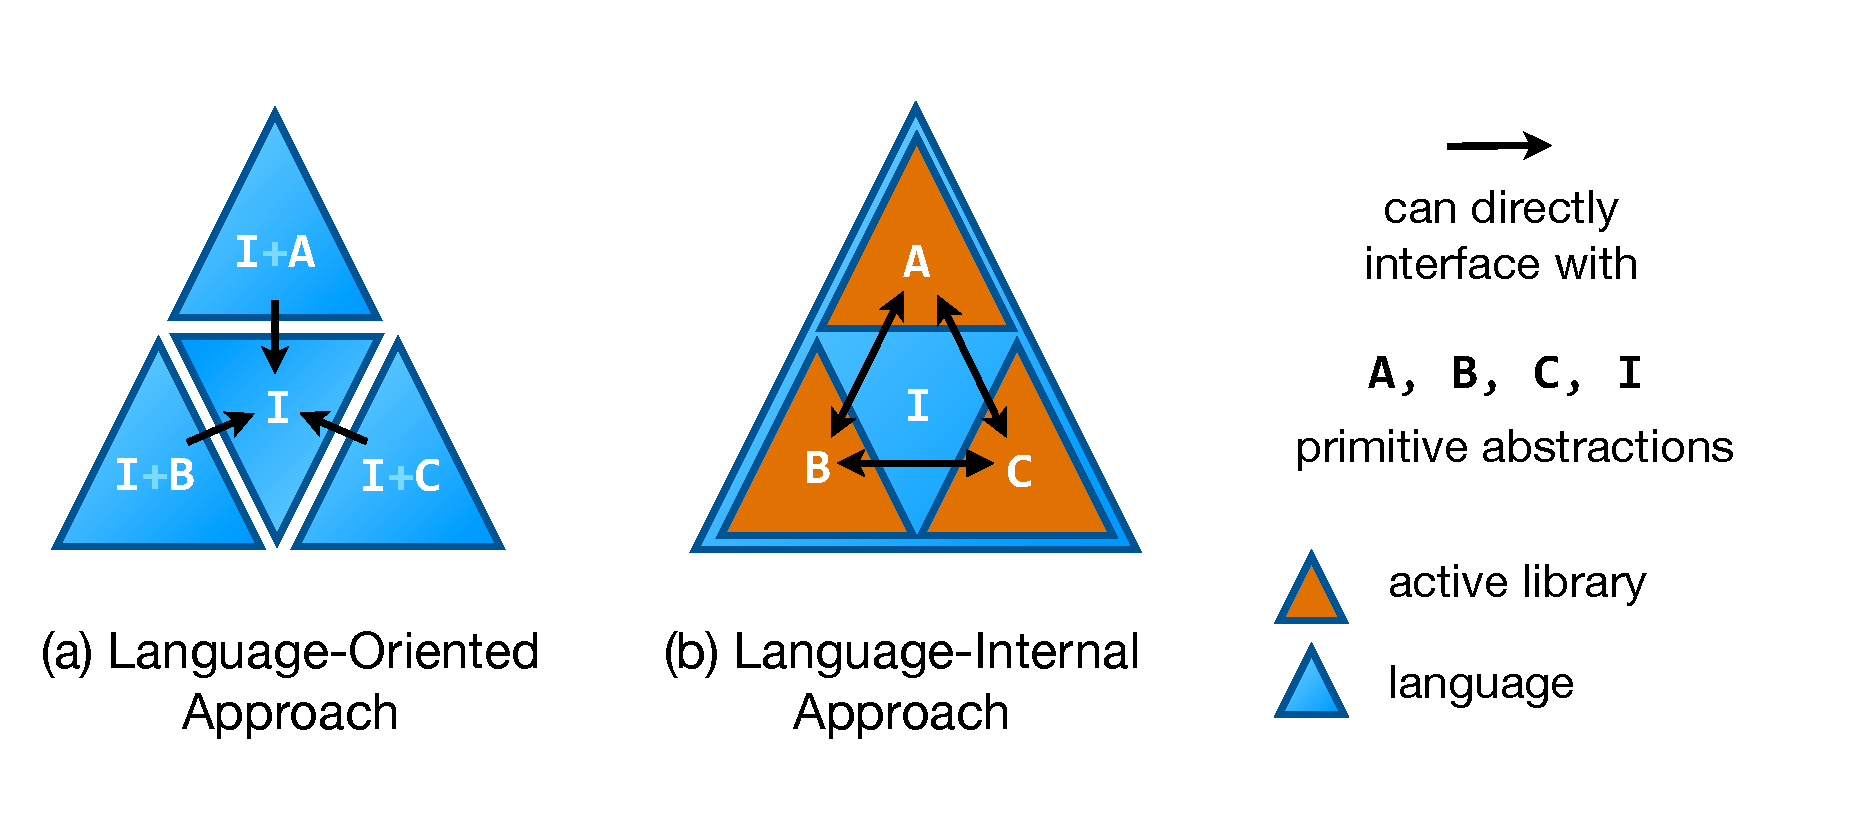
\includegraphics[scale=0.5]{approaches.pdf}
%%\end{center}
%%\vspace{-20px}
%%\caption{\small (a) With a language-oriented approach, novel constructs are packaged into separate languages. Users can only safely and naturally call into languages consisting of common constructs (often only the common target language, such as C or Java bytecode). (b) With a language-internal extensibility approach, there is one system providing a common internal language, where additional primitive constructs that strictly strengthen its static guarantees or perform specialized code generation are specified and distributed within libraries. \label{approaches}}
%%\end{figure*}
%
%%As a result, domain-specific languages and new general-purpose abstractions alike have experienced relatively slow adoption in practice.
%%
%%Porting large codebases to new languages is difficult, and the dominant programming languages innovate slowly, so programming language.
%%
%%More specifically, such languages are neither \emph{internally extensible} because the language itself exposes only natural numbers and functions to its users, nor are they \emph{externally extensible} because no new behaviors can be added to the language's  implementation in a separate module from the one containing the initial implementation.
%
%%This is the essence of a monolithic language implementation: it is impossible for anyone to modularly extend languages defined in this way. 
%
%%An extensible programming language could address these problems by providing a language-integrated mechanism for introducing new type and operator constructors and implementing their associated static and dynamic semantics directly. 
%%%Library developers need only consider which abstractions are most appropriate for their domain, without also considering whether these constructs can be exposed using abstractions appropriate to the domains of client code. Clients can simply import any necessary constructs when using a library that relies on them, preserving safety and ease-of-use without the use of  wrappers and glue code. We show this competing approach in Figure \ref{approaches}(b).
%%%Researchers and domain experts thus gain the ability to distribute new ideas for evaluation to a broader development community without requiring the approval of maintainers of mainstream languages, large-scale porting of code or explicit interoperability layers. 
%%But, as mentioned in Section \ref{language-integrated-approaches}, some significant challenges must be addressed before such a mechanism can be relied upon. The desire for expressiveness must be balanced against  concerns about maintaining various safety properties in the presence of arbitrary combinations of user-defined  extensions to the language's core semantics. The mechanism must ensure that desirable \emph{metatheoretic properties} (e.g. type safety, decidability) of the language are maintained by extensions. Because multiple independently developed extensions might be used within one program, the mechanism must further guarantee their \emph{non-interference}. These are the issues we seek to address in this work.
%
%%When designing and implementing a new abstraction, experts typically begin by attempting to define new constructs in terms of existing language constructs.
%%This approach is often effective because modern {general-purpose} abstraction mechanisms, like inductive datatypes and object systems, are highly expressive.  
%%For example, the Delite framework leverages Scala's powerful general-purpose mechanisms to enable a number of useful \emph{embedded domain-specific languages} \cite{delite}.
%%Unfortunately, there remain some situations of interest where general-purpose abstractions fall short. 
%%For instance, it is difficult to adequately encode advanced type systems in terms of the simpler rules that govern general-purpose abstractions (e.g. reasoning about units of measure requires built-in language support in F\# \cite{conf/cefp/Kennedy09}). 
%%Even if a full encoding is possible, it may not be useful if it is overly verbose or unnatural, or if the error messages are overly abstract. For example, regular expressions encoded using inductive datatypes are quite verbose, so most functional languages support them via strings, which is less safe. 
%%Finally, general-purpose abstractions are implemented in a uniform manner, meaning domain-specific heuristics cannot be applied to eliminate overhead or perform optimizations, and implementations designed for typical application workloads may not be satisfactory in parts of a program where performance is a key criteria, such as when targeting heterogeneous hardware platforms (e.g. programmable GPUs) and distributed computing resources.
%%
%%% are at times impossible or impractical. In our example of adding products or sums to Godel's T, although Church encodings are possible \cite{pfpl}, they require a reasonable level of creativity\footnote{Anecdotally, Church encodings are among the more difficult-to-explain topics covered in our undergraduate programming languages course.}. Moreover, they will not offer the same static safety guarantees as a primitive encoding, they are more verbose and they will incur performance overhead by their use of closures rather than a more direct representation. This is not only a problem for simple languages like Godel's T. Several Haskell-based embedded DSLs have also needed to make significant compromises at times \cite{haskellDSLs}. {\color{red} examples? Scala?}
%%
%%%creating a new language. If this is not practical, the best one can attempt to do is encode the new types in terms of existing types (by a Church encoding, for example). This is generally unsatisfactory -- 
%%
%%%Languages implemented using these common patterns are central planning by a language designer or design committee. 
%%
%%Researchers or domain experts who run into situations like these, where more direct control over a language's semantics and implementation are needed, have little choice today but to realize new abstractions by creating a new language in some way. They might develop a new standalone language from scratch, modify an implementation of an existing language, or use tools like compiler generators, DSL frameworks and language workbenches \cite{fowler2010domain}. 
%%%In our simple scenario, we may simply fork our implementation of Godel's T or even edit it directly (a pernicious technique for implementing a new language where the prior one is overwritten). 
%%%In a more complex scenario, we may instead employ a tool like a compiler generator or DSL framework \cite{fowler2010domain} that can generate a standalone implementation from declarative specifications of language constructs. Some of these tools allow you to package and reuse these specifications (with the important caveat that not all combinations of constructs are valid and free of conflicts, an important modularity issue that we will return to several times in this paper).
%%The increasing sophistication and ease-of-use of these tools have led to calls for a {\it language-oriented approach} to software development, where different components of an application are written in different specialized languages \cite{journals/stp/Ward94}. Indeed, a number of software ecosystems are now designed explicitly to support many different languages, both general-purpose and domain-specific, atop a common intermediate language. The Java virtual machine (JVM), the Common Language Infrastructure (CLI) and LLVM are prominent examples of such ecosystems.
%%
%%Unfortunately, this leads to a critical problem at language boundaries: a library's external interface must only use constructs that can reasonably be expressed in \emph{all possible client languages}. This discourages languages from including constructs that rely on statically-checked invariants stronger than those supported by their underlying implementation in the common intermediate language. At best, constructs like these can be exposed by generating a wrapper where run-time checks have been inserted to guarantee these invariants. This compromises both verifiability and performance. %Forrequires the development of an interoperability layer for every pair of DSLs. 
%%Moreover, this approach exposes the internals of an implementation to clients, making the abstraction awkward to work with and causing code breakage when implementation details change. This defeats a primary purpose of high-level programming languages: hiding low-level details from clients of an abstraction. We diagram this fundamental \emph{interoperability problem} in Figure \ref{approaches}(a). 
%%%As an example, F\#'s type system prevents \lstinline{null} values from occurring within data structures, but because it's type system is not available when calling into F\# code from another language, like C\#, run-time null checks must still be included in the implementation.
%%%\begin{figure*}[t]
%%%\vspace{-15px}
%%%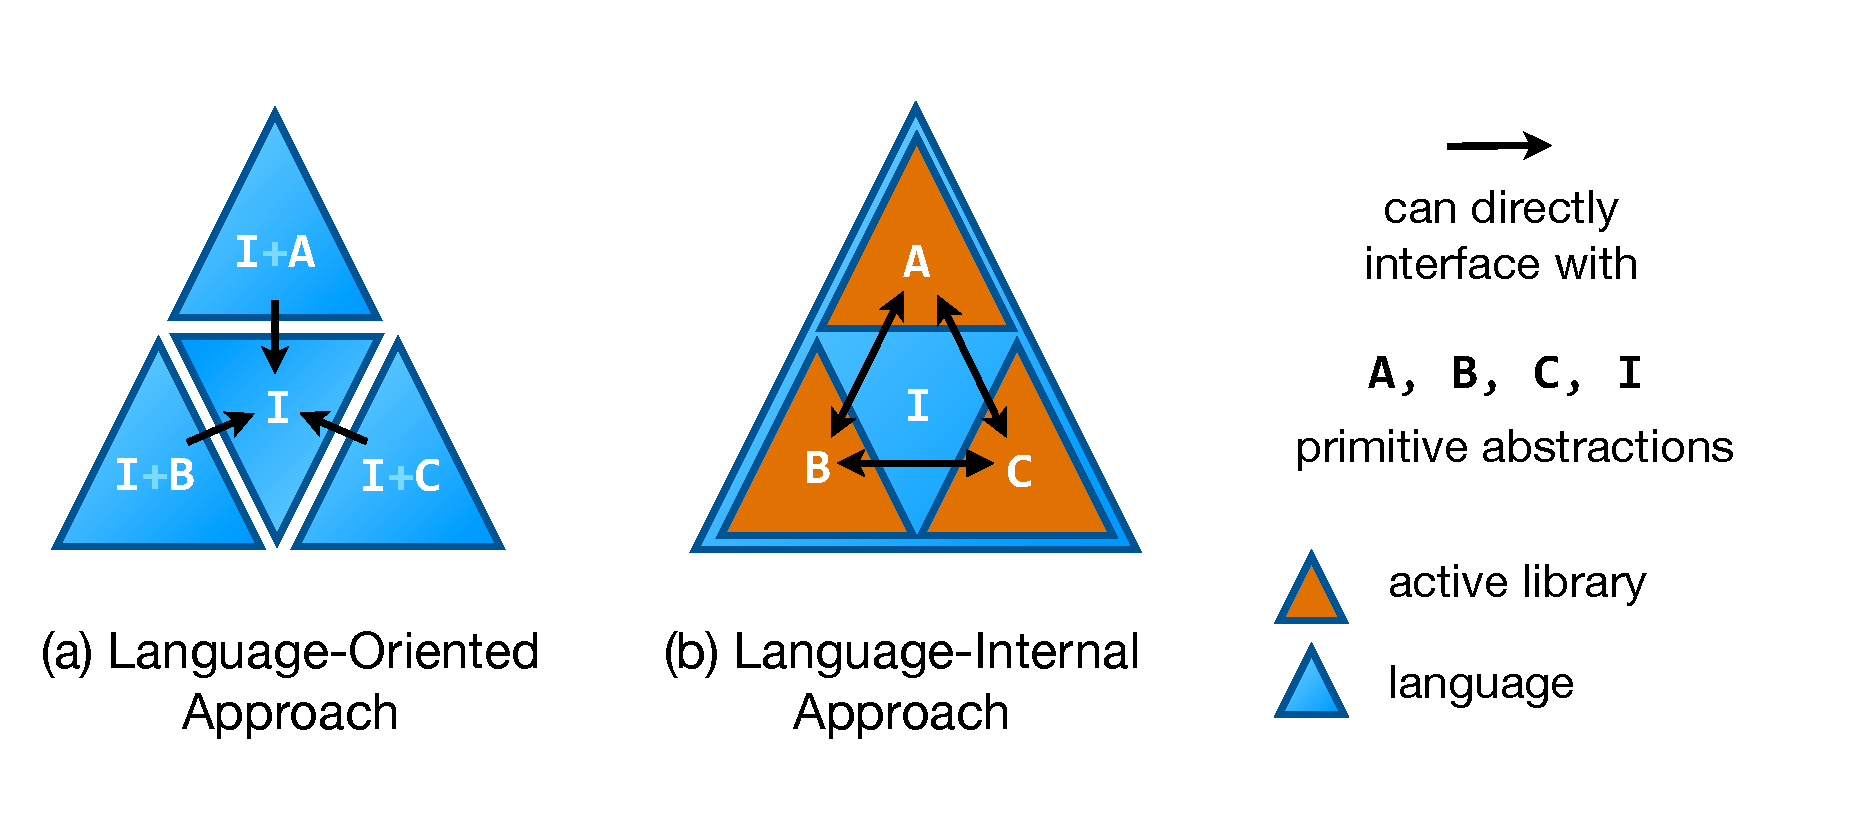
\includegraphics[scale=0.415]{approaches.pdf}
%%%\caption{(a) With the language-oriented approach, different primitive abstractions are packaged into separate languages that extend and target a common intermediate language (e.g. JVM bytecode). Users can only interface with libraries written in another language via the constructs in the common language, causing \emph{interoperability problems}. (b) With the language-internal approach, the semantics of new abstractions (i.e. the logic that governs typechecking and translation to a fixed {internal language}, here labeled \texttt{I}) can be implemented directly within so-called \emph{active libraries}. Clients can import and use these abstractions directly whenever needed.}
%%%\label{approaches}
%%%\end{figure*}
%%
%%%As a result, domain-specific languages and new general-purpose abstractions alike have experienced relatively slow adoption in practice.
%%%
%%%Porting large codebases to new languages is difficult, and the dominant programming languages innovate slowly, so programming language.
%%%
%%%More specifically, such languages are neither \emph{internally extensible} because the language itself exposes only natural numbers and functions to its users, nor are they \emph{externally extensible} because no new behaviors can be added to the language's  implementation in a separate module from the one containing the initial implementation.
%%
%%%This is the essence of a monolithic language implementation: it is impossible for anyone to modularly extend languages defined in this way. 
%%
%%%Programming languages are typically designed around a monolithic collection of primitive type families and operators. Consider, as a simple example, Godel's T \cite{pfpl}, a typed lambda calculus with recursion on primitive natural numbers\todo{add statics to Appendix A}. Although a language designer may casually speak of ``extending Godel's T with primitive product and sum types'', adding these type families and associated operators to this kind of language from within is impossible. That is, Godel's T is not \emph{internally extensible}.
%%
%%\emph{Internally-extensible programming languages} promise to avoid these problems by providing researchers and domain experts with a mechanism for implementing the semantics of new primitive constructs directly within libraries.
%%%Developers of libraries need only determine whether they are appropriate for their domain, without also considering whether these constructs can be exposed in terms of abstractions appropriate to client code. 
%%As a result, clients can granularly import any necessary primitive constructs when using code that relies on them, and thereby achieve full safety, ease-of-use and performance. Providers of components thus need only consider whether primitives that they use are appropriate for their domain, without also considering whether their code might be used in a context where these primitives are not otherwise appropriate. Libraries containing logic that is invoked at compile-time, as extension logic would be, have been called \emph{active libraries} \cite{activelibraries}. We adopt this terminology and diagram this competing approach in Figure \ref{approaches}(b).
%%
%%%Researchers and domain experts thus gain the ability to distribute new ideas for evaluation to a broader development community without requiring the approval of maintainers of mainstream languages, large-scale porting of code or explicit interoperability layers. 
%%
%%For a language-internal extension mechanism to be feasible, however, it must achieve expressiveness while also ensuring that extensions cannot compromise the safety properties of the language and its tools, nor interfere with one another. That is, extensions cannot simply be permitted to add arbitrary logic to the type system or compiler, because this would make it possible to break  type safety, decidability or adequacy theorems that are critical to the operation of the language, the compiler or other extensions. We review some previous attempts at language extensibility, and highlight how they do not adequately achieve both safety and expressiveness, in Section \ref{related-work}.
%%%{\color{red} transition here} Correctness properties of an extension itself should be modularly verifiable, so that its users can rely on it for verifying and compiling their own code. The mechanism must also ensure that desirable metatheoretic properties and global safety guarantees of the language cannot be weakened by extensions. And with multiple independently-developed extensions used at once, the mechanism must further guarantee that they cannot interfere with one another. 
%%
%%In this paper, we introduce a language-internal extensibility mechanism called \emph{active typechecking and translation} (AT\&T) that allows developers to introduce and implement the logic governing new primitive type and operator families from within libraries. 
%%We argue that this can be accomplished by enriching the type-level language, rather than introducing a separate metalanguage into the system. 
%%To make this proposal concrete, we begin by introducing a simple core calculus, called \atlam~(for the ``actively-typed lambda calculus''), in Section \ref{atlam}. 
%%This calculus uses type-level computation of higher kind, along with techniques borrowed from the typed compilation literature and a form of type abstraction that ensures that the implementation details of an extension are not externally visible to guarantee the safety of the language, the decidability of typechecking and compilation and non-interference of extensions, as we outline in Section \ref{safety}.
%%In Section \ref{examples}, we suggest that despite these constraints, this mechanism is expressive enough to admit, within libraries, a number of general-purpose and domain-specific abstractions that normally require built-in language support. 
%%
%%Our core calculus uses a uniform abstract syntax for primitive operators to simplify our presentation and analysis, but this syntax is too verbose to be practical. Thus, we begin this section by showing how a key design choice made in the calculus -- to associate operators with type families, forming what we call \emph{active type families} -- supports a novel type-directed desugaring mechanism that permits the use of conventional concrete syntax for language extensions. 
%
%% Our choice of a simply-typed, simply-kinded calculus where expressions are given meaning by translation to a simply-typed internal language appears to occupy a ``sweet spot'' in the design space, and relates closely to how simply-typed functional languages like  ML and Haskell are specified and implemented today. In Section \ref{design}, we briefly discuss other points in the design space of actively-typed languages and describe the sorts of abstractions that the mechanism as we have introduced it is not capable of expressing, suggesting several directions for future research. We conclude with a discussion of related work in Section \ref{related-work}.
%%dependently-typed and object-oriented type-level languages, as well as the constraints governing the design of the internal language.  
%%We will also note how object-oriented techniques may also be suit, because of a fundamental connection to the \emph{expression problem} \cite{expression-problem}.
%
%%specify new typechecking rules and translation logic from within libraries. The AT\&T mechanism utilizes type-level computation of higher kind and integrates typed compilation techniques into the language to provide strong safety guarantees, while remaining straightforward and expressive.
%
%%AT\&T is general with respect to many choices about the type-level language, the typed internal language and syntax. Choices along these dimensions can affect both expressiveness and ease-of-use. We will begin in Sec. 2 by introducing a minimal system called $@\lambda$ (the ``actively-typed lambda calculus'') that distills the essence of the mechanism in a simply-typed, simply-kinded setting. This will allow us to fully and concisely formalize the language and compiler and give several key safety theorems. We will then continue in Sec. 3 by discussing variants of this mechanism based on other basic paradigms, considering dependently-typed functional languages and object-oriented languages, discussing trade-offs between expressivity and safety when doing so. We have developed a simple prototype called Ace and have used it to develop a number of full-scale language extensions as libraries. We will briefly discuss this language and these extensions in Sec. 4.
%
%%We note at the outset that AT\&T focuses on extending the static semantics of languages with fixed, though flexible, syntax. Language-internal syntax extension mechanisms have been developed in the past (e.g. SugarJ \cite{sugarj}) but they have also suffered from safety problems because grammar composition is not always safe when done in an  unconstrained manner. Constrained approaches that provide stronger safety guarantees have recently been outlined (e.g. Wyvern \cite{globaldsl13}) but we will leave integration of syntax extensions with semantic extensions as future work.
%%\section{From Extensible Compilers to Extensible Languages}\label{evolution}
%%\begin{figure}[t]
%%\small
%%$$\begin{array}{rccl}	
%%\textbf{programs} & \rho & ::= & \pfam{\familyDf}{\progsort}  \\
%% & & \pipe &  \pdef{t}{\kappa}{\tau}{\progsort} \pipe e\\
%%\text{primitive ops}		&	\theta	&	::= &	\tops{op}{\kappaidx}{i}{a}{\tau} \pipe 
%%												\topp{\theta}{\theta}\\
%%\\
%%\textbf{external terms} 				&	e	&	::=	&	\evar{x} \pipe 
%%														\elam{\evar{x}}{\tau}{e} \pipe 
%%														\eop{Fam}{op}{
%%															\taui
%%														}{
%%  												    		\splat{e}{1}{n}
%%														} \\
%%									& 		&		& 	\\
%%							
%%\hspace{-5pt}\textbf{type-level terms} 	& \tau 	& ::= 	& 	\tvar{t} \pipe 
%%														\tlam{t}{\kappa}{\tau} \pipe 
%%														\tapp{\tau_1}{\tau_2}\pipe
%%														\iintlit \pipe \iop{\tau_1}{\tau_2} \pipe \tstr{str} \\
%%									    & &  \pipe & 
%%														\tnil{\kappa} \pipe \tcons{\tau_1}{\tau_2} \pipe 
%%									                     \tfold{\tau_1}{\tau_2}{h}{t}{r}{\tau_3}
%%														\\
%%												
%%	 			& 		& \pipe	& 	 \tunit \pipe 
%%														\tpair{\tau_{1}}{\tau_{2}} \pipe 
%%														\tfst{\tau} \pipe 
%%														\tsnd{\tau} 
%%														\\
%%\text{equality}  & & \pipe & 					\tifeq{\tau_{1}}{\tau_{2}}{\kappa}{\tau_{3}}{\tau_{4}} 
%%														\\														
%%
%%\text{types} 						& 		& \pipe	& 	\ttypestd \\
%% & & \pipe &  \tfamcase{\tau}{Tycon}{x}{\tau_1}{\tau_2}\\
%%						%				& & \pipe & \tfamcase{\tau}{Fam}{x}{\tau_1}{\tau_2}\\
%%																								
%%\text{denotations} 				& 		 & 	\pipe	&	\tden{\tauiterm}{\tautype} \pipe \terr \\
%% & & \pipe &  \tdencase{\tau}{x}{t}{\tau_1}{\tau_2}\\
%% %& & \pipe & 
%%%														\tdencase{\tau}{y}{x}{\tau_1}{\tau_2}
%%%														 \\
%%
%%\text{reified IL}		&		&	\pipe	&	\titerm{\iota} \pipe \titype{\sigma} \\
%%
%%												\\
%%\textbf{kinds} 					& \kappa	&	::=	&	\karrow{\kappa_1}{\kappa_2} \pipe \klist{\kappa} \pipe \dint \pipe
%%											    \kstr \pipe
%%												\kunit \pipe 
%%												\kpair{\kappa_{1}}{\kappa_{2}} \\
%%	& & \pipe &  
%%												\kTypeBlur \pipe \kDen \pipe 
%%												\kIType \pipe \kITerm
%%												\\
%%\\												
%%%\textbf{ops signature}			& \Theta	&	::=	&	\kOpEmpty \pipe \kOp{\Theta}{op}{\kappai}\\
%%%											 							&		&		&	\\
%%\textbf{internal terms} 				& 	\iota	&	::=	&	\evar{x} \pipe 
%%												\ilam{\evar{x}}{\sigma}{\iota} \pipe 
%%												\iapp{\iota_{1}}{\iota_{2}} \pipe
%%												\ifix{\evar{f}}{\sigma}{\iota} \\
%%									& & \pipe & 
%%												\ipair{\iota_{1}}{\iota_{2}} \pipe 
%%												\ifst{\iota} \pipe
%%												\isnd{\iota}  
%%												\\
%%							& 		& 	\pipe	& 
%%												\iintlit \pipe \iop{\iota_{1}}{\iota_{2}} \pipe \iIfEq{\iota_{1}}{\iota_{2}}{\dint}{\iota_{3}}{\iota_{4}}  
%%												\\
%% &  & \pipe & \tvalof{\tau_1}{\tau_2} \pipe \iup{\tau} \\
%%%\text{deabstracted}& \iota & ::= & \mathcal{G}[\iota, \sigma]\\
%%\textbf{internal types}			&	\sigma	&	::=	&    \darrow{\sigma_1}{\sigma_2} \pipe
%%												\dint \pipe
%%												\dpair{\sigma_1}{\sigma_2} \pipe
%%												\trepof{\tau} \pipe \dup{\tau}\\
%%\end{array}$$
%%%\vspace{-10pt}
%%\caption{\small Syntax of \atlam. Variables $x$ are used in expressions and internal terms and are distinct from type-level variables, $\tvar{t}$. Names $\fvar{Fam}$ are type family names (we assume that globally unique type family names can be generated by some external mechanism) and $\opvar{op}$ are operator family names. $\tstr{str}$ denotes string literals, $\iintlit$ denotes integer literals and $\oplus$ stands for binary operations over integers. %The productions related to the internal language are written using generators $\mathcal{G}$ and $\mathcal{S}$ to avoid duplicating the syntax of common terms.
%%\label{grammar}}
%%\end{figure}
%%\begin{figure}[t]
%%\small
%%\begin{flalign}
%%\label{natfam}&\family{Nat}{\kunit}{\\
%%\label{z}&\quad\tops{z}{\kunit}{i}{a}{
%%	\tapp{\tapp{\tvar{empty}}{\tvar{a}}}{
%%		\tden{\titerm{0}}{\ttype{Nat}{\tunit}}
%%	}};\\
%%\label{s}&\quad\tops{s}{\kunit}{i}{a}{
%%	\tapp{
%%		\tapp{\tvar{pop\_final}}{\tvar{a}}}{\tlam{x}{\kITerm}{\tlam{t}{\kTypeBlur}{
%%			\\
%%			&\quad\quad\tapp{\tapp{\tapp{\tvar{check\_type}}{\tvar{t}}}{\ttype{Nat}{\tunit}}}{
%%				\tden{\titerm{\iup{\tvar{x}}+1}}{\ttype{Nat}{\tunit}}
%%			}
%%		}}
%%		}
%%	};\\
%%\label{rec}&\quad\tops{rec}{\kunit}{i}{a}{
%%	\tapp{\tapp{\tvar{pop}}{\tvar{a}}}{\tlam{x1}{\kITerm}{\tlam{t1}{\kTypeBlur}{\tlam{a}{\klist{\kDen}}{\\
%%	&\quad\quad\tapp{\tapp{\tvar{pop}}{\tvar{a}}}{\tlam{x2}{\kITerm}{\tlam{t2}{\kTypeBlur}{\tlam{a}{\klist{\kDen}}{\\
%%	&\quad\quad \tapp{\tapp{\tvar{pop\_final}}{\tvar{a}}}{\tlam{x3}{\kITerm}{\tlam{t3}{\kTypeBlur}{\\
%%	&\quad\quad \tapp{\tapp{\tapp{\tvar{check\_type}}{\tvar{t1}}}{\ttype{Nat}{\tunit}}}{(\\
%%	&\quad\quad \tapp{\tapp{\tapp{\tvar{check\_type}}{\tvar{t3}}}{\ttype{Arrow}{(\ttype{Nat}{\tunit},\ttype{Arrow}{(\tvar{t2},\tvar{t2})})}}}{\\
%%		\label{fix}&\quad\quad \tden{\titerm{\iapp{(\ifix{f}{\darrow{\dint}{\trepof{\tvar{t2}}}}{\ilam{x}{\dint}{\\
%%		\label{lastop}&\quad\quad\quad \iIfEq{x}{0}{\dint}{\iup{\tvar{x2}}}{\iapp{\iapp{\iup{\tvar{x3}}}{(x-1)}}{(\iapp{f}{(x-1)})}}}})}{\iup{\tvar{x1}}}}}{\tvar{t2}}
%%	)}}
%%	}}}}}}}}}}}}
%%\\
%%&}{XXX}{i}{\titype{\dint}};\\
%%\label{nattype}&\pdef{nat}{\kTypeBlur}{\ttype{Nat}{\tunit}}{\\
%%\label{plus}&(\elam{plus}{\ttype{Arrow}{(\tvar{nat}, \ttype{Arrow}{(\tvar{nat}, \tvar{nat}))}}}{
%%	\elam{two}{\tvar{nat}}{\\
%%\label{ap}	&\quad\quad \eopapp{\eopapp{plus}{two}}{two}}})
%%}\\
%%\label{add}&\quad (\elam{x}{\tvar{nat}}{\elam{y}{\tvar{nat}}{
%%	\eop{Nat}{rec}{\tunit}{x; y; \elam{p}{\tvar{nat}}{\elam{r}{\tvar{nat}}{
%%	\eop{Nat}{s}{\tunit}{r}
%%	}}}}})\\
%%\label{two}&\quad  \eop{Nat}{s}{\tunit}{\eop{Nat}{s}{\tunit}{\eop{Nat}{z}{\tunit}{ }}}
%%%{\\&\elet{two}{\tvar{nat}}{\eop{Nat}{s}{\tunit}{\eop{Nat}{s}{\tunit}{\eop{Nat}{z}{\tunit}{ }}}}{\eapp{\eapp{plus}{two}}{two}}}
%%%}
%%%\elam{x}{\tvar{nat}}{\elam{y}{\tvar{nat}}{\\
%%	%&\quad \eop{Nat}{rec}{\tunit}{x; y; \elam{p}{\tvar{nat}}{\elam{r}{\tvar{nat}}{
%%	%\eop{Nat}{s}{\tunit}{r}
%%	%}}}}
%%\end{flalign}
%%\caption{G\"odel's T in \atlam, used to calculate 2+2. Helper functions for working with lists ($\tvar{empty}$, $\tvar{pop}$, $\tvar{pop\_final}$) and types ($\tvar{check\_type}$),  described below, are given in the appendix. We will refer to this program as $\rho_{\text{nat}}$ in the text.}
%%\label{example}
%%\end{figure}
%%
%%To understand the genesis of our internal extension mechanism, it is helpful to begin by considering why most implementations of programming languages cannot even be  externally extended. 
%%Let us consider, as a simple example, an implementation of G\"odel's T, a typed lambda calculus with recursion on primitive natural numbers (see Appendix). 
%%A compiler for this language written using a functional language will invariably represent the primitive type families and operators using {closed} inductive datatypes. 
%%For example, a simple implementation in Standard ML may be based around these datatypes:
%%\begin{lstlisting}
%%  datatype Type = Nat | Arrow of Type * Type
%%  datatype Exp = Var of var 
%%               | Lam of var * Type * Exp | Ap of Exp * Exp 
%%               | Z | S of Exp | Natrec of Exp * Exp * Exp
%%\end{lstlisting}
%%
%%The logic governing typechecking and translation to a suitable intermediate language (for subsequent optimization and compilation by some back-end) will proceed by exhaustive case analysis over the constructors of \lstinline{Exp}.
%%
%%In an object-oriented implementation of Godel's T, we might instead encode types and operators as subclasses of abstract classes \lstinline{Type} and \lstinline{Exp}. Typechecking and translation will proceed by the ubiquitous \emph{visitor pattern}  by dispatching against a fixed collection of {known} subclasses of \lstinline{Exp}. 
%%
%%In either case, we encounter the same basic issue: there is no way to modularly add new primitive type families and operators and implement their associated typechecking and translation logic. 
%%%This issue is related to the widely-discussed \emph{expression problem} (in a restricted sense -- we do not consider adding new functions beyond typechecking and translation here, only adding logic to these) \cite{wadler-expression}.
%%
%%A number of language mechanisms have been proposed that allow new cases to be added to datatypes and the functions that operate over them in a modular manner. 
%%In functional languages, we might use \emph{open datatypes}. For example, if we wish to extend G\"odel's T with product types and we have written our compiler in a language supporting open inductive datatypes, it might be possible to add new cases like this: 
%%\begin{lstlisting}
%%  newcase Prod of Type * Type extends Type
%%  newcase Pair of Exp * Exp extends Exp    (* Intro *)
%%  newcase PrL of Exp extends Exp           (* Elim Left *)
%%  newcase PrR of Exp extends Exp           (* Elim Right *)
%%\end{lstlisting}
%%
%%The logic for functionality like typechecking and translation could then be implemented for only these new cases. For example, the \lstinline{typeof} function that assigns a type to an expression could be extended like so:
%%\begin{lstlisting}
%%  typeof PrL(e) = case typeof e of 
%%      Prod(t1, _) => t1 
%%    | _ => raise TypeError("<appropriate error message>")
%%\end{lstlisting}
%%
%%If we allowed users to define new modules containing definitions like these and link them into our compiler, we will have succeeded in creating an externally-extensible compiler, albeit one where safety is not guaranteed (we will return to this point shortly). We have not, however, created an extensible programming language, for two reasons. First, compiler extensions are distributed and activated separately from libraries, so dependencies become more difficult to manage. Second, other compilers for the same language will not necessarily support the same extensions. 
%%If our newly-introduced constructs are exposed at a library's  interface boundary, clients using different compilers face the same problems with interoperability that those using different languages face. That is, {extending a language by extending a single compiler for it is morally equivalent to creating a new language}. Several prominent language ecosystems today are in a state where a prominent compiler has introduced or enabled the introduction of extensions that many libraries have come to rely on, including the Glasgow Haskell Compiler, SML/NJ and the GNU compilers for C and C++.
%%
%%A more appropriate and useful place for extensions like this is directly within libraries, alongside abstractions that can be adequately implemented in terms of existing primitive abstractions. To enable this, the language must allow for the introduction new primitive type families, like \lstinline{Prod}, operators, like \lstinline{Pair}, \lstinline{PrL} and \lstinline{PrR}, and associated typechecking and translation logic. When encountering these new operators in expressions, the compiler must effectively  hand control over typechecking and translation to the appropriate user-defined logic. Because this mechanism is {language-internal}, all compilers must support it to satisfy the language specification.
%%
%%Statically-typed languages typically make a distinction between \emph{expressions}, which describe run-time computations, and type-level constructs like types, type aliases and datatype declarations. The design described above suggests we may now need to add another layer to our language, an {extension language}, where extensions can be declared and implemented. In fact, we will show that \textbf{the most natural place for type system extensions is within the type-level language}. The intuition is that extensions to a statically-typed language's semantics will need to manipulate types as values at compile-time. Many languages already allow users to write type-level functions for various reasons, effectively supporting this notion of types as values at compile-time (see Sec. \ref{related-work} for examples). The type-level language is often constrained by its own type system (where the types of type-level values are called \emph{kinds} for clarity) that prevents type-level functions from causing problems during compilation. This is precisely the structure that a distinct extension layer would have, and so it is quite natural to unify the two, as we will show in this work.
%%
%%\section{\atlam}\label{atlam}
%%In this section, we will develop a core calculus, called @$\lambda$ for the ``actively-typed lambda calculus'', by way of a semantics and a simple example, and discuss how it addresses the safety concerns that arise. 
%%\subsection{Overview}
%%The grammar of \atlam~is shown in Figure \ref{grammar}. 
%%A program, $\rho$, consists of a series of declarations followed by an expression. Declarations can be either bindings of type-level terms to type-level variables using \textsf{def} or a primitive type family declared using \textsf{family}, which can contain implementations of one or more operator families, $\theta$. Expressions, $e$, can be either variables, lambdas, or applications of operators.
%%%, and are ultimately given meaning by translation to a typed internal language, with terms $\iota$ and types $\sigma$. 
%%%This language has been chosen, for simplicity, to be a variant of Plotkin's PCF with primitive integers and products, but in practice would include other constructs consistent with its role as a high-level intermediate language.
%%
%%The language is structured as a simply-typed lambda calculus with simply-kinded type-level computation. Kinds, $\kappa$, classify type-level terms, $\tau$. 
%%Types are type-level values of kind $\star$ (following System $F_{\omega}$) and classify expressions. The type-level language also includes other kinds of terms: type-level functions, lists (required by our mechanism), integers, strings and products for the sake of our examples (see Sec. \ref{safety} for a discussion on other acceptable kinds of type-level data) and constructs for developing extensions -- denotations and reified internal terms and types -- which we will discuss in the sections below. 
%%
%%All expressions are given meaning by translation to a typed internal language. This language has been chosen, for simplicity, to be a variant of Plotkin's PCF with primitive integers and products, but in practice would include other constructs consistent with its role as a high-level intermediate language. The grammar of internal terms, $\iota$, and internal types, $\sigma$, also includes special forms containing type-level terms; these are used for developing extensions and during compilation and will be erased before compilation ends.
%%\subsection{Example: G\"odel's T as an Active Type Family}
%%To make our explanation of each of the constructs in the calculus concrete, we will work through an example showing how to introduce primitive natural numbers with bounded recursion in the style of G\"odel's T \cite{pfpl}. These will be implemented internally as integers (that is, internal terms of internal type $\dint$). Figure \ref{example} shows how to define the indexed type family $\fvar{Nat}$. This family contains only one type, written $\ttype{Nat}{\tunit}$, which we alias on line \ref{nattype} by defining the type-level variable $\tvar{nat}$. We define the typechecking and translation logic for the operators associated with this family (\opvar{z}, \opvar{s} and \opvar{rec}) on lines \ref{z}-\ref{lastop} and use these to define a $plus$ function on line \ref{add} and compute 2+2. We will refer back to this figure as we describe each construct below.
%%
%%\subsection{Indexed Type Families and Types}\label{families}
%%The syntactic form $\familyDf$ declares a new primitive type family named $\fvar{Fam}$ indexed by type-level values of kind $\kappaidx$ with representation schema $\tvar{i}.\taurep$ and operators $\theta$. The purpose of the representation schema and of associating of operators directly with types will be explained below. 
%%
%%Declaring a type family in this way is a language-internal analog to adding a new constructor to the compiler-internal datatype \lstinline{Type}, as suggested in Sec. \ref{evolution}. 
%%The index represents the data associated with this constructor. A type (that is, a type-level term of kind $\kTypeBlur$) is constructed by naming a family in scope and providing a type-level term of the appropriate kind as an index. A base type like $\tvar{nat}$ can be thought of as being the only type in the family $\fvar{Nat}$ trivially indexed by the unit value, of kind $\kunit$, while families like $\fvar{Ntuple}$ might be indexed by a list of types, having kind $\klist{\kTypeBlur}$. 
%% For example, $\ttype{Ntuple}{\tcons{\tvar{nat}}{\tcons{\tvar{nat}}{\tnil{\kTypeBlur}}}}$ might be the type of a pair of natural numbers. Given a type, its family can be \textsf{case} analyzed to extract the value of its index. It is important that type equality be decidable, so only kinds for which equivalence coincides with syntactic equality can be used as type family indices. The main  consequence of this restriction is that indices cannot contain type-level functions.
%%
%%\subsection{Representations and Representation Schemas}
%%As we will discuss further below, it is important that all expressions classified by a type compile to consistently-typed internal terms. For this reason, we require that every type have a single internal type associated with it, called its \emph{representation}. This is computed by substituting the type index for the bound variable $\tvar{i}$ in the term $\taurep$, called the \emph{representation schema} of the type family, and evaluating to a value representing an internal type. Internal types, $\sigma$, are reified as type-level terms of kind $\kIType$ using the introductory form $\titype{\sigma}$.
%%
%%\subsection{Indexed Operator Families and Denotations}\label{operators}
%%Type families are also equiped with a collection of primitive operator families. An operator family named $\opvar{op}$ is declared using the form $\tops{op}{\kappaidx}{i}{a}{\tauop}$. Like type families, operator families are indexed by values of some kind, $\kappaidx$, but because operators are not first-class type-level values in our calculus, there are no equality restrictions. In the example in Fig. \ref{example}, all the operators are trivially indexed by the kind $\kunit$, so each family only contains one operator. However, a type family like $\fvar{Ntuple}$ would be equipped with a family of projection operators, $\opvar{pr}$, indexed by a position (e.g. an integer in our calculus). A family implementing record types or object types might have a similar operator indexed by a type-level string representing the field being accessed (see Sec. \ref{examples}).
%%
%%To apply an operator, the grammar provides a uniform form of expression: $\eop{Fam}{op}{\tauidx}{e_1; \ldots; e_n}$, where $n \geq 0$. The typechecking and translation of an expression of this form is controlled by the term $\tauop$ in the operator's declaration. This term must evaluate to a \emph{denotation}, which is a type-level value of kind $\kDen$, when given the operator index, $\tauidx$, and a list constructed from the denotations recursively assigned to each argument, $e_1$ through $e_n$. 
%%
%%There are two forms of denotations that an expression can be assigned. A \emph{valid denotation} has the form $\tden{\tauiterm}{\tautype}$, where $\tauiterm$ is the \emph{translation} of the expression to an internal term and $\tautype$ is the type it has been assigned. Internal terms are represented as type-level terms using the form $\titerm{\iota}$, and have kind $\kITerm$ (similar to $\kIType$). %It is important to note that there are no elimination form for reified terms or types.
%%%(indeed, in \atlam, terms are never  syntactically analyzed directly by extensions, unlike macro systems and other forms of term rewriting; see Sec. \ref{related-work})
%%If a type error is detected by an operator, the \emph{error denotation}, $\terr$, is returned instead of a valid denotation. In a practical implementation, a specialized error message and other diagnostic information would be provided when returning $\terr$, but we omit such details for simplicity. Terms of kind $\kDen$ can be \textsf{case} analyzed to determine if they are valid or errors, and if valid, to extract the translation and type.
%%
%%In the example in Fig. \ref{example}, the operator $\opvar{z}$ checks that no arguments were passed in using the simple helper function $\tvar{empty}$. If so, it returns a valid denotation by pairing the translation $\titerm{0}$ with the type $\ttype{Nat}{\tunit}$, as expected\footnote{Actually, there is no theoretical barrier to a different ``zero'' being used!}. If an argument was provided, the helper function returns $\terr$. The successor operator, $\opvar{s}$, takes one argument, so it pops a denotation off the argument list, making sure there are no more, and binds its translation and type to $\tvar{x}$ and $\tvar{t}$ respectively, all using the helper function $\tvar{pop\_final}$. It then checks that the argument's type is also $\ttype{Nat}{\tunit}$, returning a denotation pairing the translation $\titerm{\iup{\tvar{x}} + 1}$ with the type $\ttype{Nat}{\tunit}$ if so. The form $\iup{\tau}$ is used to ``un-reify'' reified internal terms, of kind $\kITerm$ (thus serving as the left-inverse of $\titerm{\iota}$). In this case, $\tvar{x}$ is a type-level variable of kind $\kITerm$ representing the translation of the argument to the successor operator, so we simply need to add one to it. Because we have checked that the denotation's type was $\ttype{Nat}{\tunit}$, and the representation schema will guarantee that expressions of this type always translate to integers, we know that it is safe to do so. If any of these steps fail, the various helper functions we use simply return $\terr$ (in practice, it would be prudent to equip each failure condition with a different error message). Compilation will also fail if we accidentally violate the representation schema, as we will see in Sec. \ref{repcon}.
%%
%%% The operator index, $\tauidx$, and . 
%%
%%\subsection{Functions, Variables and Arrow Types}
%%
%%The recursor operator, $\opvar{rec}$, proceeds similarly, extracting the translations and types of each of its three arguments. Of note, however, is how it handles the third argument, which binds two variables (the predecessor and the result of recursing on it). In \atlam, the built-in $\lambda$ operator serves as the sole mechanism for introducing bound variables. In most calculi, lambda terms have types of the form $\tau_1 \rightarrow \tau_2$. In \atlam, $\rightarrow$ corresponds to the built-in type family, $\fvar{Arrow}$. This family is indexed by a pair of types, $\kpair{\kTypeBlur}{\kTypeBlur}$, and is always in scope. Its representation schema simply maps to the corresponding internal arrow type, $\tvar{i}.\titype{\darrow{\trepof{\tfst{\tvar{i}}}}{\trepof{\tsnd{\tvar{i}}}}}$. The special form $\trepof{\tau}$ is used to refer, abstractly, to the representation of the type $\tau$ (we also see this used on line \ref{fix}). Although the $\lambda$ operator is built-in, because it needs to bind variables, application is just an operator associated with the $\fvar{Arrow}$ family, $\opvar{ap}$, as is seen on line \ref{ap}. The details are straightforward and given in the appendix.
%%
%%\subsection{Compilation}
%%\begin{figure}[t]
%%\small
%%\begin{mathpar}
%%\inferrule{
%%	\overbrace{\progOK{\emptyctx}{\fvalCtx_0}{\rho}}^{\text{\normalsize Kind Checking}}\\
%%	\overbrace{\pcompiles{\fvalCtx_0}{\rho}{\iota}}^{\text{\normalsize Active Typechecking and Translation}}
%%}{
%%	\ptcc{\rho}{\iota}
%%}
%%\end{mathpar}
%%\caption{\small Central Compilation Judgement of \atlam.}
%%\label{ccj}
%%\end{figure}
%%The \emph{central compilation judgement}, shown in Figure \ref{ccj}, captures the two phases of compilation: kind checking and active typechecking and translation. 
%%The first phase ensures that all type-level terms in the program are well-kinded and that all expressions and internal terms are closed. The kinding rules for programs are given in Figure \ref{kindprog}, and they rely on the kinding rules for type-level terms given in Figure \ref{tlkind}. These rules use contexts $\Sigma$ and $\Theta$ to track family and operator signatures, but beyond that, the rules are largely consistent with those of a simply-typed lambda calculus shifted into the type-level, with the addition of the handful of special forms constrained as described in the previous sections. The reader is encouraged to verify that the example in Fig. \ref{example} is well-kinded. 
%%% As we will see, the kind checking phase ensures that many kinds of errors are ruled out and that this process will not ``get stuck'' (see Sec. \ref{safety}). The evaluation semantics for type-level terms are given in Fig. \ref{tleval}.
%%\begin{figure}[t]
%%\small
%%$\fbox{\inferrule{}{\progOKX{\progsort}}}$
%%~~~$\tvarCtx ::= \emptyctx \pipe \tvarCtxX{t}{\kappa}$~~~
%%$\fCtx ::= \Sigma_0	 \pipe \fvalCtxX$
%%\begin{mathpar}
%%\inferrule[family-kinding]{
%%	\fvar{Fam} \notin \text{dom}(\fvalCtx)\\
%%	\kEq{\kappaidx}\\
%%	\opType{\tvarCtx}{\fvalCtxX}{\theta}{\Theta}\\\\
%%	\tKind{\tvarCtx, \tvar{i}:{\kappaidx}}{\fvalCtxX}{\tau}{\kIType}\\
%%	\progOK{\tvarCtx}{\fvalCtxX}{\rho}
%%}{
%%	\progOKX{\pfam{\familyDf}{\rho}}
%%}
%%
%%\inferrule[def-kinding]{
%%	\tKindX{\tau}{\kappa}\\
%%	\progOK{\tvarCtxX{t}{\kappa}}{\fvalCtx}{\rho}
%%}{
%%	\progOKX{\pdef{t}{\kappa}{\tau}{\rho}}
%%}
%%
%%\inferrule[exp-kinding]{
%%	\exprOK{\tvarCtx}{\emptyctx}{\fvalCtx}{e}
%%}{
%%	\progOKX{e}
%%}
%%\end{mathpar}
%%$\fbox{$\tKindX{\theta}{\Theta}$}$
%%~~~$\Theta ::= \kOpS{op}{\kappaidx} \pipe \Theta, \Theta$~~~
%%\begin{mathpar}
%%\inferrule[op-kinding]{
%%	\tKind{\tvarCtx, \tOfKind{\tvar{i}}{\kappai}, \tOfKind{\tvar{a}}{\klist{\kDen}}}{\fvalCtx}{\tau}{\kDen}
%%}{
%%	\opType{\tvarCtx}{\fvalCtx}{{\tops{op}{\kappaidx}{i}{a}{\tau}}}{
%%	\kOpS{op}{\kappaidx}}
%%}
%%
%%\inferrule[ops-kinding]{
%%	\tKindX{\theta_1}{\Theta_1}\\
%%	\tKindX{\theta_2}{\Theta_2}\\\\
%%	\text{dom}(\theta_1) \cap \text{dom}(\theta_2) = \emptyset
%%}{
%%	\tKindX{\theta_1; \theta_2}{\Theta_1, \Theta_2}
%%}
%%\end{mathpar}
%%$\fbox{$\exprOKX{e}$}$
%%~~~$\itvarCtx ::= \emptyctx \pipe \itvarCtx, \evar{x}$
%%\begin{mathpar}
%%\inferrule[e-var-kinding]{ }{
%%	\exprOK{\tvarCtx}{\itvarCtx, \evar{x}}{\fvalCtx}{\evar{x}}
%%}
%%
%%\inferrule[e-lam-kinding]{
%%	\tKindX{\tau}{\kTypeBlur}\\
%%	\exprOK{\tvarCtx}{\eivarCtxX{x}}{\fvalCtx}{e}
%%}{
%%	\exprOKX{\elam{\evar{x}}{\tau}{e}}
%%}
%%
%%\inferrule[e-op-kinding]{
%%	\fvarOfType{Fam}{\kappaidx}{\Theta} \in \fvalCtx\\
%%	\kOpS{op}{\kappai} \in \Theta\\
%%	\tKindX{\taui}{\kappai}\\\\
%%	\exprOKX{e_1}\\
%%	\cdots\\
%%	\exprOKX{e_n}
%%}{
%%	\exprOKX{\eop{Fam}{op}{\taui}{\splat{e}{1}{n}}}
%%}
%%\end{mathpar}
%%\caption{\small Kinding for programs. Variable contexts $\tvarCtx$ and $\itvarCtx$ obey standard structural properties. Kinding rules for type-level terms are given in Figure \ref{tlkind}.}
%%\label{kindprog}
%%\vspace{-10pt}
%%\end{figure}
%%%\subsection{Active Typechecking and Translation}
%%The second phase of compilation involves invoking the  logic implemented by user-defined operator families to typecheck and translate the program. The rules for this phase are given in Fig. \ref{att}. The context $\fvalCtx$ tracks the operator definitions and representation schemas associated with families in scope. Because the logic inside operators must be invoked during this phase, we need an evaluation semantics for type-level terms, given in Fig. \ref{tleval}. This is again a largely unsurprising collection of rules with the exception of \textsc{dencase-eval-valid}, which we will explain below.
%%
%%\subsection{Abstract Representations and Abstract Internal Types}\label{repcon}
%%To typecheck and translate an expression, $e$, the rule \textsc{att-exp} first assigns a type, $\tau$, and an \emph{abstract translation}, $\gabs$, to it, as determined by the judgement $\ecompilesX{e}{\tau}{\gabs}$. It then \emph{deabstracts} this abstract translation to complete the compilation process, as determined by the judgement $\eraseX{\gabs}{\iota}$. The purpose of the abstract translation phase is to ensure that the implementation details of type families are not exposed to other families, so that invariants that they rely on are preserved when families are composed. For example, our implementation of natural numbers as integers in Fig. \ref{example} maintains the invariant that the translation is non-negative. If the knowledge that natural numbers are implemented as integers was externally visible, a different extension could introduce an operator like $\tops{badnat}{\kunit}{i}{a}{\tapp{\tvar{const}}{\tapp{\tvar{a}}{\tden{\titerm{-1}}{\ttype{Nat}{\tunit}}}}}$, breaking this invariant (and thus the guarantee that the recursor always terminates!) 
%%%To put it another way, if a collection of operators can be shown to be a full and faithful (that is, adequate) encoding of a particular type system, then it does not matter what other types there are in the system.
%%
%%We preclude such operations by a mechanism similar to the abstract type mechanism supported by ML-style module systems \cite{pfpl}. By keeping a type family's representation schema private to the operators associated with it, they maintain full control over representation invariants. So, because it cannot be shown given the knowledge available in the type family containing $\opvar{badnum}$ that the internal type associated with $\ttype{Nat}{\tunit}$ is $\dint$, the translation $-1$ will not be permitted according to the rules we will give below. The only way to produce a term of type $\ttype{Nat}{\tunit}$ as the result of applying an operator not associated with the family $\fvar{Nat}$ is if that operator extracts the term from an argument (e.g. when projecting it out of an $n$-tuple), in which case the necessary invariants are inductively  maintained (see Sec. \ref{safety}). Translations extracted from denotations via \textsf{case} analysis are tracked during this phase as \emph{abstract internal terms}, $\tvalof{\tau_1}{\tau_2}$ (see rule \textsc{dencase-eval-valid}).%
%%
%%Let us first review how expressions are assigned types and abstract translations. Variables (\textsc{att-var}) translate directly to variables in the internal language, with the type determined by the typing context, $\iota$. Lambda terms (\textsc{att-lam}) also translate to lambda terms in the internal language and are given the appropriate $\fvar{Arrow}$ type by extending the typing context and proceeding recursively as is usual. The internal type of the argument, however, is left as $\trepof{\tau_1'}$, which is called the \emph{abstract representation} of $\tau_1'$. The actual representation of this type is only available from within operators in its family.
%%
%%Now we will consider the important operator application rule (\textsc{att-op}). This rule operates by extracting the appropriate operator definition, evaluating the operator index to a value, $\tauidx'$, and recursively assigning a type and abstract translation to each argument. From these, it constructs a list of denotations  and passes this list, along with the fully evaluated operator index, to the  operator implementation, $\tauop$. If this results in a valid denotation, compilation can proceed, but if an $\terr$ is produced, compilation will stop because no other rule will apply (in practice, we would display a type error at this point).
%%
%%Before a valid denotation produced in this way can be used, however, we check that it is \emph{representationally consistent}, meaning that the abstract translation, $\gabs$, is of an abstract internal type consistent with the abstraction representation of the type it is paired with, $\tau$. The premise $\ddbar{\Xi_0,\fvar{Fam}}{\fvalCtx}{\trepof{\tau}}{\sabs}$ determines the abstract internal type and the premise $\checkRC{\gtCtx}{\Xi_0,\fvar{Fam}}{\fvalCtx}{\gabs}{\sabs}$ performs the internal type checking. To do so, the variable context, $\iota$, which associates variables with types, must be converted to a context associating those variables with their corresponding abstract internal types, $\gtCtx$. The relevant judgements are defined in Fig. \ref{ait}. The schema context $\Xi$ is used to track which representation schemas are visible. In our calculus, $\Xi_0=\fvar{Arrow}$ is always visible alongside the schema of the family associated with the operator being considered. This could be exanded to support module-scoped visibility (we do not include modules in our calculus for simplicity), mutually-defined type families or type families that intentionally expose their representation schemas publicly (as $\fvar{Arrow}$ does).
%%
%%To clarify this fundamental mechanism let us examine how the expression $\eop{Nat}{s}{\tunit}{\eop{Nat}{z}{\tunit}{ }}$ will be processed during this phase. The inner application of $\opvar{z}$ will produce the abstract translation $0$ paired with the type $\ttype{Nat}{\tunit}$. Because the representation schema for $\fvar{Nat}$ is available, we have that $\ddbar{\Xi_0,\fvar{Nat}}{\fvalCtx}{\trepof{\ttype{Nat}{\tunit}}}{\dint}$ by \textsc{show-rep}, as needed. In contrast, if $\opvar{badnat}$ were used inside, the representation schema of $\fvar{Nat}$ would not be available, so we can only apply \textsc{hide-rep}, which does not give us enough information to give $-1$ a type.  
%%
%%When the compiler next considers the outer application of $\opvar{s}$, it will pass the denotation $\tden{\titerm{0}}{\ttype{Nat}{\tunit}}$ into its definition.  There, it binds the translation to the variable $\tvar{x}$ (within the $\tvar{pop\_final}$ helper function). However, $\tvar{x}$ is not simply $\titerm{0}$. Instead, its provenance is tracked by using the form $\tvalof{\titerm{0}}{\ttype{Nat}{\tunit}}$. When attempting to check that $\iup{\tvar{x}} + 1$ is valid, the \textsc{show-trans} rule will reveal that it is an integer because, again, the appropriate representation schema is available. If the schema were not available, the most that could be derived is that $\checkRC{\gtCtx}{\Xi}{\fvalCtx}{\iup{\tvar{x}}}{\trepof{\ttype{Nat}{\tunit}}}$. The fact that natural numbers are represented using integers is not derivable (though it is true), so the addition operation would fail to type. This fact would, however, be sufficient for implementing families, like $\fvar{Ntuple}$, that do not require knowledge about a type's representation. We encourage the reader to derive these judgements for the logic in the $\opvar{rec}$ operator to strengthen their understanding of this fundamental mechanism.
%%
%%We cannot leave abstract representations and abstract internal terms in the result of compilation, so a final deabstraction phase erases these, replacing them with their underlying internal types and terms in all contexts. Just as with abstract types in modules or existential types, there is no run-time overhead to this mechanism -- programs run at full speed. We give the deabstraction rules in the appendix due to their simplicity.
%%
%
%%
%
%%
%%\begin{figure}[t]
%%\small
%%$\fbox{\inferrule{}{\concrep{\fvalCtx}{\tau}{\sigma}}}$
%%\begin{mathpar}
%%\inferrule[get-rep]{
%%	\fval{Fam}{\theta}{i}{\tau} \in \fvalCtx\\
%%	\tEvalX{[\tauidx/\tvar{i}]\tau}{\titype{\sigma}}\\
%%	\ddbarX{\sigma}{\sconc}
%%}{
%%	\concrep{\fvalCtx}{\ttype{Fam}{\tauidx}}{\sconc}
%%}
%%\end{mathpar}
%%$\fbox{\inferrule{}{\ddbarX{\sigma}{\sigma'}}}$
%%~~~$\fvalCtx ::= \fvalCtx_0 \pipe \fvalCtx, \fvalDf$~~~
%%~~~$\Xi ::= \Xi_0 \pipe \Xi, \fvar{Fam}$~~~
%%~~~$\Xi_0 := \fvar{Arrow}$
%%\begin{mathpar}
%%\inferrule[abs-int]{ }{
%%	\ddbarX{\dint}{\dint}
%%}
%%
%%\inferrule[abs-arrow]{
%%	\ddbarX{\sigma_1}{\sigma_1'}\\
%%	\ddbarX{\sigma_2}{\sigma_2'}
%%}{
%%	\ddbarX{\darrow{\sigma_1}{\sigma_2}}{\darrow{\sigma_1'}{\sigma_2'}}
%%}
%%
%%\inferrule[abs-prod]{
%%	\ddbarX{\sigma_1}{\sigma_1'}\\
%%	\ddbarX{\sigma_2}{\sigma_2'}
%%}{
%%	\ddbarX{\dpair{\sigma_1}{\sigma_2}}{\dpair{\sigma_1'}{\sigma_2'}}
%%}
%%
%%\inferrule[itype-inverse]{
%%	\ddbarX{\sigma}{\sabs}
%%}{
%%	\ddbarX{\dup{\titype{\sigma}}}{\sabs}
%%}
%%
%%\inferrule[show-rep]{
%%	\fvar{Fam} \in \Xi\\
%%	\concrep{\fvalCtx}{\ttype{Fam}{\tauidx}}{\sconc}
%%}{
%%	\ddbarX{\trepof{\ttype{Fam}{\tauidx}}}{\sconc}
%%}
%%
%%\inferrule[hide-rep]{
%%	\fvar{Fam} \notin \Xi
%%}{
%%	\ddbarX{\trepof{\ttype{Fam}{\tauidx}}}{\trepof{\ttype{Fam}{\tauidx}}}
%%}
%%\end{mathpar}
%%$\fbox{\inferrule{}{\eCtxTogCtxX{\etCtx}{\gtCtx}}}$
%%~~~$\gtCtx ::= \emptyctx \pipe \gtCtxX{x}{\sigma}$
%%\begin{mathpar}
%%\inferrule[abs-empty]{ }{
%%	\eCtxTogCtxX{\emptyctx}{\emptyctx}
%%}
%%
%%\inferrule[abs-ctx]{
%%	\eCtxTogCtxX{\etCtx}{\gtCtx}\\
%%	\ddbarX{\trepof{\tau}}{\sigma}
%%}{
%%	\eCtxTogCtxX{\etCtxX{x}{\tau}}{\gtCtxX{x}{\sigma}}
%%}
%%\end{mathpar}
%%$\fbox{\inferrule{}{\checkRCX{\iota}{\sigma}}}$
%%\begin{mathpar}
%%\inferrule[abs-i-var]{ }{
%%	\checkRC{\gtCtxX{x}{\sigma}}{\Xi}{\fvalCtx}{\evar{x}}{\sigma}
%%}
%%
%%\inferrule[abs-i-lam]{
%%	\ddbarX{\sigma_1}{\sigma_1'}\\
%%	\checkRC{\gtCtxX{x}{\sigma_1'}}{\Xi}{\fvalCtx}{\iota}{\sigma_2}
%%}{
%%	\checkRCX{\ilam{x}{\sigma_1}{\iota}}{\darrow{\sigma_1'}{\sigma_2}}
%%}
%%
%%\inferrule[abs-i-ap]{
%%	\checkRCX{\iota_1}{\darrow{\sigma_1}{\sigma_2}}\\
%%	\checkRCX{\iota_2}{\sigma_1}
%%}{
%%	\checkRCX{\iapp{\iota_1}{\iota_2}}{\sigma_2}
%%}
%%
%%\inferrule[abs-i-fix]{
%%	\ddbarX{\sigma}{\sigma'}\\
%%	\checkRC{\gtCtxX{x}{\sigma'}}{\Xi}{\fvalCtx}{\iota}{\sigma'}
%%}{
%%	\checkRCX{\ifix{x}{\sigma}{\gabs}}{\sigma'}
%%}
%%\\
%%\text{\color{gray} (standard statics for integers and products omitted)}
%%\\
%%%\inferrule[abs int]{ }{
%%%	\checkRCX{\iintlit}{\dint}
%%%}
%%%
%%%\inferrule[abs op]{
%%%	\checkRCX{\iota_1}{\dint}\\
%%%	\checkRCX{\iota_2}{\dint}
%%%}{
%%%	\checkRCX{\iop{\iota_1}{\iota_2}}{\dint}
%%%}
%%%
%%%\inferrule[abs pair]{
%%%	\checkRCX{\iota_1}{\sigma_1}\\
%%%	\checkRCX{\iota_2}{\sigma_2}
%%%}{
%%%	\checkRCX{\ipair{\iota_1}{\iota_2}}{\dpair{\sigma_1}{\sigma_2}}
%%%}
%%%
%%%\inferrule[abs fst]{
%%%	\checkRCX{\iota}{\dpair{\sigma_1}{\sigma_2}}
%%%}{
%%%	\checkRCX{\ifst{\iota}}{\sigma_1}
%%%}
%%%
%%%\inferrule[abs snd]{
%%%	\checkRCX{\iota}{\dpair{\sigma_1}{\sigma_2}}
%%%}{
%%%	\checkRCX{\isnd{\iota}}{\sigma_2}
%%%}
%%%
%%% \inferrule[abs-int-eq]{
%%% 	\checkRCX{\iota_1}{\dint}\\
%%% 	\checkRCX{\iota_2}{\dint}\\\\
%%% 	\checkRCX{\iota_3}{\sigma}\\
%%% 	\checkRCX{\iota_4}{\sigma}
%%% }{
%%% 	\checkRCX{\iIfEq{\iota_1}{\iota_2}{\dint}{\iota_3}{\iota_4}}{\sigma}
%%% }
%%\inferrule[abs-iterm-inverse]{
%%	\checkRCX{\iota}{\sigma}
%%}{
%%	\checkRCX{\iup{\titerm{\iota}}}{\sigma}
%%}
%%
%%\inferrule[show-trans]{
%%	\fvar{Fam} \in \Xi\\
%%	\concrep{\fvalCtx}{\ttype{Fam}{\tauidx}}{\sigma}\\
%%	\checkRCX{\iota}{\sigma}
%%}{
%%	\checkRCX{\tvalof{\titerm{\iota}}{\ttype{Fam}{\tauidx}}}{\sigma}
%%}
%%
%%\inferrule[hide-trans]{
%%	\fvar{Fam} \notin \Xi\\
%%	\concrep{\fvalCtx}{\ttype{Fam}{\tauidx}}{\sigma}\\
%%	\checkRCX{\iota}{\sigma}
%%}{
%%	\checkRCX{\tvalof{\titerm{\iota}}{\ttype{Fam}{\tauidx}}}{\trepof{\ttype{Fam}{\tauidx}}}
%%}
%%\end{mathpar}
%%\caption{\small Abstracted internal typing}
%%\label{ait}
%%\end{figure}
%%%
%%%family RECORD of (string, type) dict {
%%%  new(idx, args. foldl (fn (x, y) => 
%%%  get[field : string](idx. case find(idx, field) of SOME t => t | _ => err)
%%
%%\section{Safety of @$\lambda$}\label{safety}
%%In giving users of a language direct influence on the typechecking and translation of expressions, it is essential to consider safety properties. It must not be possible for well-typed programs to fail to finish compiling or go wrong at run-time because of a buggy extension. It is also considered desirable for typechecking to be decidable. And for extensions to be reliable, they must not be allowed to interfere with one another under any circumstance. By carefully designing our extension mechanism, we believe we have achieved each of these goals.
%%
%%\subsection{Representational Consistency and Type Safety}
%%We do not need to give a semantics to internal terms and internal types that do not survive deabstraction. The remaining terms and types form a variant of PCF with well-understood primitives (here, integers and binary products) known to be type safe \cite{pfpl}. If compilation can be shown to always result in a well-typed term of this language, then type safety follows by composing these two facts. Fortunately, this fact is a corollary of our representational consistency mechanism, described in Sec. \ref{repcon}. The proof is by straightforward (though deeply nested!) rule induction.
%%
%%%\begin{theorem}[Representational Consistency]
%%%If $\progOK{ }{\Sigma}{e}$ and $\ecompiles{ }{\fvalCtx}{e}{\tau}{\gabs}$ and $\eraseX{\gabs}{\iota}$ and 	$\ddbar{\Xi_0}{\fvalCtx}{\trepof{\tau}}{\sabs}$ and $\eraseX{\sabs}{\sigma}$ then $\checkRC{ }{\Xi_0}{\fvalCtx}{\iota}{\sigma}$. 
%%%\end{theorem}
%%
%%\subsection{Decidability}
%%To show that compilation is decidable, we need to show that both kind checking and active typechecking and compilation are decidable. This hinges on showing that the type-level language is typesafe and that evaluation of type-level terms always terminates. 
%%
%%%\begin{theorem}[Kind Safety and Termination]
%%%If $\vdash_{\Sigma} \tau : \kappa$ then $\tEvalX{\tau}{\tau'}$ such that $\vdash_{\Sigma_0} \tau' : \kappa$ and $\tEvalX{\tau'}{\tau'}$. 
%%%\end{theorem}
%%
%%The proof is straightforward because the type-level language is based on a conventional simply-typed lambda calculus with only bounded recursion over lists, so standard techniques (e.g. logical relations) can be used directly. The only new constructs are the types, denotations and reified internal language forms, but because none of these can contain type-level functions by the statics, there is no risk of introducing self-reference by their inclusion. If the type-level language included constructs like inductive datatypes (without a strict positivity condition) or general recursion, this theorem would be weakened.
%%
%%\subsection{Non-Interference}
%%Our abstraction mechanism guarantees that the representation invariants collectively maintained by the operators associated with a type family cannot be violated by operators in other type families, by ensuring that introductory forms cannot be defined outside the family. One way to state this is as follows:
%%
%%%\begin{theorem}[Non-Interference]
%%%For any property $P(\iota)$, if $\progOK{ }{\Sigma}{e}$ and $\ecompiles{ }{\fvalCtx}{e}{\tau}{\gabs}$ and $\eraseX{\gabs}{\iota}$ implies $P(\iota)$, then for any $\Sigma'$ and $\fvalCtx'$ disjoint from $\Sigma$ and $\fvalCtx$, we have that if $\progOK{ }{\Sigma,\Sigma'}{e'}$ and $\ecompiles{ }{\fvalCtx,\fvalCtx'}{e'}{\tau}{\gabs'}$ and $\eraseX{\gabs'}{\iota'}$ then $P(\iota')$.
%%%\end{theorem}
%%The proof relies on the fact that the show/hide rules are mutually exclusive and so there are two cases to consider for each form of expression, and weakening properties of the family contexts. This powerful theorem allows us to compose type families arbitrarily without needing to handle cases in our implementation that are ruled out based on a local analysis. The details will be provided in the appendix.
%%
%%% \subsection{Modular Verification}
%%% nope
%%
%%% that's all folks
%%
%%\section{Use Cases}\label{examples}
%%
%%Aldrich argues that dynamic dispatch has proven useful for building  large software frameworks \cite{aldrich-onward13}. Object-oriented languages support dynamic dispatch directly but encodings of dynamic dispatch in terms of standard functional primitives can be awkward and difficult to reason about (e.g. \cite{pfpl} Ch. X).
%%
%%Indexed type families and indexed operator families are a powerful tool for programming language semantics. In \emph{Practical Foundations for Programming Languages}, for example, nearly every chapter defines a new collection of indexed types and operators and gives their semantics in isolation from the constructs in the other chapters \cite{pfpl}. For example, $n$-ary sums and products are families indexed by a list of types. Labeled variants of these simply pair the labels with the types as static strings. Even nested pattern matching, such as that found in modern functional languages, can be understood as an operator family indexed by a series of patterns, which can be represented as type-level data. In the appendix, we show how to implement sums and products in \atlam. 
%%
%%The book also shows constructs as varied as dynamic types as well as a number of constructs for parallelism and concurrency, such as futures, promises and actors. With a sufficiently capable internal language (exposing basic concurrency primitives, for example), each of these could be fully implemented as libraries using our mechanism. Few languages include primitive support for several such abstractions, even though they are often useful together. In a preliminary implementation of this calculus, Ace, which is beyond the scope of this paper, we have implemented the entirety of the OpenCL programming language as a library, along with primitives supporting partitioned global address spaces.
%%
%%Object systems too could be implemented using this mechanism, with indices serving to capture the inheritance data and the signatures. Operator families for reading and writing fields and/or sending messages would be parameterized by strings naming them. The operator definition would simply search the signatures going up the inheritance hierarchy, and implement objects in a conventional way (e.g. using a v-table together with a pointer to a structure containing field data). A variety of object systems could coexist within the same language. Another related example would be to implement a safe and efficient interoperability layer with an existing OO language by capturing its type system as an extension, to be used only at language boundaries.
%%
%%Finally, a variety of domain-specific type systems, capturing complex rule systems like the system of scientific units of measure (a family indexed by the measure being used and the type which the measure is being applied to), regular expressions \cite{regexp} (a family indexed by the number of captured groups) or XML \cite{xml} (indexed by a document schema) would be possible. Recent work examined a specialized type system capturing the semantics of the widely-used jQuery javascript library \cite{jquery-oopsla}. Today, these all require \emph{ad hoc} language-external solutions, or the development of new languages. 
%%
%%%\section{Design Considerations}\label{design}
%%
%\section{Related Work}\label{related-work}
%Our representation schema abstraction mechanism relates closely to abstract and existential types \cite{pfpl,atpl}. Our calculus enforces the abstraction barriers  in a purely syntactic manner, as in previous work on syntactic type abstraction \cite{syntypeabs}. While this work is all focused on abstracting away the identity of a particular type outside of the ``principal'' it is associated with (e.g. a module), we focus on abstracting away the knowledge of how a primitive type family is implemented outside of a limited scope.
%
%The representational consistency mechanism brings into the language work on typed compilation, especially work done on Standard ML in the TILT project \cite{tilt}. Indeed, the specification of Standard ML is structured around a typed internal language and a judgement that assigns a type and an internal term to each expression \cite{smlstd}. Representational consistency is related to the notion of type-directed copmilation in this work.
%
%Type-level computation is supported in some form by a growing number of languages. For example, Haskell supports a simple form of it \cite{Chakravarty:2005:ATC}). Ur uses type-level records and names to support typesafe metaprogramming, with applications to web programming \cite{conf/pldi/Chlipala10}. $\Omega$mega adds algebraic data types at the type-level, using these to increase the expressive power of algebraic data types at the expression level \cite{conf/cefp/SheardL07}. Dependently-typed languages blur the traditional phase separation between types and expressions, so type-level computation is often implicitly used (though not always in its most general form, e.g. Deputy \cite{conf/icfp/ChenX05}, ATS \cite{conf/esop/ConditHAGN07}). We show how to integrate language extensions into the type-level language, drawing on ideas about \cite{activelibraries}.
%
%% \subsection{Run-Time Indirection}
%% {\it Operator overloading} \cite{vanWijngaarden:Mailloux:Peck:Koster:Sintzoff:Lindsey:Meertens:Fisker:acta:1975} and {\it metaobject dispatch} \cite{Kiczales91} are run-time protocols that translate operator invocations into function calls. The function is typically selected according to the type or value of one or more operands. These protocols share the notion of {\it inversion of control} with type-level specification. However, type-level specification is a {\it compile-time} protocol focused on enabling specialized verification and implementation strategies, rather than simply enabling run-time indirection.
%
%Many languages and tools allow developers to rewrite expressions according to custom rules. These can broadly be classified as {\it term rewriting systems}. Macro systems, such as those characteristic of the LISP family of languages \cite{mccarthy1978history}, are the most prominent example. Some compile-time metaprogramming systems also allow users to manipulate syntax trees (e.g. MetaML \cite{Sheard:1999:UMS}), and external rewrite systems also exist for many languages.
%These facilities differ from AT\&T in that they involve direct manipulation of terms, while AT\&T involves extending typechecking and translation logic directly. We also draw a distinction between the type-level, used to specify types and compile-time logic, the expression grammar, used to describe run-time behavior, and the internal language, used to implement this behavior. By doing so, each component can be structured and constrained as appropriate for its distinct role, as we have shown.
%
%Previous work on extensible languages has suffered from problems with either expressiveness or safety. For example, a number of projects, such as SugarJ \cite{erdweg2011sugarj}, allow for user-defined desugarings (and indeed, our system would clearly benefit from integration with such a mechanism), but this does not allow the semantics to be fundamentally extended nor for implementation details to be hidden. Recent variants of this work has investigated introducing new typing rules, but only if they are admissible by the base type system \cite{erdwegicfp}. Our work allows for entirely new logic to be added to the system, requiring only that the implementation of this logic respect the internal type system. A number of other extensible languages (e.g. Xroma \cite{xroma}) and compilers do allow new static semantics to be introduced, but in an unconstrained manner based on global pattern matching and rewriting, leading to significant problems with interference and safety. Our work aims to provide a sound and safe underpinning, based around well-understood concepts of type and operator families, to language extensibility.
%
%In the future, we will investigate mechanisms to enable type systems with specialized binding and scoping rules, as well as integration of dependent kinds to support mechanized verification of key properties like representational consistency and adequacy against a declarative specification at kind-checking time. We will also investigate mechanisms that enable a more natural syntax (e.g. Wyvern's type-directed syntax \cite{globaldsl}). 
%
%%\item With type-level specification, dispatch to a type-level function occurs implicitly on the basis of the structure of an expression. In contrast, most term-rewriting systems operate by  explicit invocation of a macro or specialized syntax. Some LISP macro systems have explored pattern-based dispatch (e.g. A*\cite{fowler2010domain}, EPP\cite{fowler2010domain}) and macro systems for object-oriented languages, like OpenC++ \cite{fowler2010domain} and OpenJava \cite{fowler2010domain}, do offer a somewhat limited form of operation-based dispatch.
%
%% \subsection{Language Frameworks}
%% When the mechanisms available in an existing language prove insufficient, researchers and domain experts must design a new language. A number of tools have been developed to assist with this task, including compiler generators, language workbenches and domain-specific language frameworks (cf \cite{fowler2010domain}).
%
%% A major barrier to adoption is the fact that interoperability is intrinsically problematic. Even languages which target a common platform, such as the Java Virtual Machine, can only interact using its limited set of primitives. Specialized typing rules are not checked at language boundaries, performance often suffers, and the syntax can be unnatural, particularly for languages which differ significantly from the platform's native language (e.g. Java).
%
%% Instead of focusing on defining standalone languages, type-level specification gives greater responsibility in a granular manner to libraries. In this way, a range of constructs can coexist within the same program and, assuming that it can be shown by some method that various constructs are safely composable, be mixed and matched. The main limitation is that the protocol requires defining a fixed source grammar, whereas a specialized language has considerable flexibility in that regard. Nevertheless, as Ace shows, a simple grammar can be used quite flexibly.
%% \subsection{Extensible Compilers}
%% An alternative methodology is to implement language features granularly as compiler extensions. As discussed in Section 1, existing designs suffer from the same problems related to composability, modularity\-, safety and security as extensible languages, while also adding the issue of language fragmentation.
%
%% Type-level specification can in fact be implemented within a compiler, rather than provided as a core language feature. This would resolve some of the issues, as described in this paper. However, by leveraging type-level computation to integrate the protocol directly into the language, we benefit from common module systems and other shared infrastructure. We also avoid the fragmentation issue.
%% \subsection{Specification Languages}
%% Several {\it specification languages} (or {\it logical frameworks}) based on these theoretical formulations exist, including the OBJ family of languages (e.g. CafeOBJ \cite{Diaconescu-Futatsugi01}). They provide support for verifying a program against a language specification, and can automatically execute these programs as well in some cases. The  language itself specifies which verification and execution strategies are used.
%
%% Type-determined compilation takes a more concrete approach to the problem, focusing on combining {\it implementations} of different\- logics, rather than simply their specifications. In other words, it focuses on combining {\it type checkers} and {\it implementation strategies} rather than more abstract representations of a language's type system and dynamic semantics. In Section 4, we outlined a preliminary approach based on proof assistant available for the type-level language to unify these approaches, and we hope to continue this line of research in future work.
%
%% CANT GUARANTEE THAT SPECIFICATIONS ARE ACTUALLY DECIDABLE
%\begin{figure}
%\small
%$\fbox{$\tEvalX{\tau}{\tau'}$}$
%\begin{mathpar}
%\inferrule[n-t-lam]{ }{
%	\tEvalX{\tlam{t}{\kappa}{\tau}}{\tlam{t}{\kappa}{\tau}}
%}
%
%\inferrule[n-t-ap]{
%	\tEvalX{\tau_1}{\tlam{t}{\kappa}{\tau}}\\
%	\tEvalX{\tau_2}{\tau_2'}\\
%	\tEvalX{\subst{\tau_2'}{\tvar{t}}{\tau}}{\tau'}
%}{
%	\tEvalX{\tapp{\tau_1}{\tau_2}}{\tau'}
%}
%
%\text{\color{gray} (normalization for integers, labels, lists, products and sums also standard)}
%
%\inferrule[n-t-eq-equal]{
%	\tEvalX{\tau_1}{\tau_1'}\\
%	\tEvalX{\tau_2}{\tau_1'}\\
%	\tEvalX{\tau_3}{\tau_3'}
%}{
%	\tEvalX{\tifeq{\tau_1}{\tau_2}{\kappa}{\tau_3}{\tau_4}}{\tau_3'}
%}
%
%\inferrule[n-t-eq-disequal]{
%	\tEvalX{\tau_1}{\tau_1'}\\
%	\tEvalX{\tau_2}{\tau_2'}\\\\
%	\tau_1' \neq \tau_2'\\
%	\tEvalX{\tau_4}{\tau_4'}
%}{
%	\tEvalX{\tifeq{\tau_1}{\tau_2}{\kappa}{\tau_3}{\tau_4}}{\tau_4'}
%}
%
%\inferrule[nt-ty]{
%	\tEvalX{\tauidx}{\tauidx'}
%}{
%	\tEvalX{\ttype{Tycon}{\tauidx}}{\ttype{Tycon}{\tauidx'}}
%}
%
%\inferrule[nt-tycase-match]{
%	\tEvalX{\tau}{\ttype{Tycon}{\tauidx}}\\
%	\tEvalX{\subst{\tauidx}{\tvar{x}}{\tau_1}}{\tau_1'}
%}{
%	\tEvalX{\tfamcase{\tau}{Tycon}{x}{\tau_1}{\tau_2}}{\tau_1'}
%}
%
%\inferrule[nt-tycase-fail]{
%	\tEvalX{\tau}{\ttype{Tycon'}{\tauidx}}\\
%	\fvar{Tycon} \neq \fvar{Tycon'}\\
%	\tEvalX{\tau_2}{\tau_2'}
%}{
%	\tEvalX{\tfamcase{\tau}{Tycon}{x}{\tau_1}{\tau_2}}{\tau_2'}
%}
%
%\inferrule[nt-d]{
%	\tEvalX{\tau}{\tau'}\\
%	\tiEvalX{\ibar}{\ibar'}
%}{
%	\tEvalX{\tden{\ibar}{\tau}}{\tden{\ibar'}{\tau'}}
%}
%
%\inferrule[nt-d-checked]{
%	\tEvalX{\tau}{\tau'}\\
%	\tiEvalX{\ibar}{\ibar'}
%}{
%	\tEvalX{\tden{\ibar}{\tau}^\checkmark}{\tden{\ibar'}{\tau'}^\checkmark}
%}
%
%\inferrule[nt-typeof]{
%	\tEvalX{\tau}{\tden{\ibar}{\tau'}}
%}{
%	\tEvalX{\ttypeof{\tau}}{\tau'}
%}
%
%\inferrule[nt-typeof-checked]{
%	\tEvalX{\tau}{\tden{\ibar}{\tau'}^\checkmark}
%}{
%	\tEvalX{\ttypeof{\tau}}{\tau'}
%}
%
%\inferrule[nt-reptype]{
%	\tiEvalX{\sbar}{\sbar'}
%}{
%	\tEvalX{\titype{\sbar}}{\titype{\sbar'}}
%}
%\end{mathpar}
%$\fbox{$\tiEvalX{\ibar}{\ibar'}$}$
%\begin{mathpar}
%\inferrule[nt-i-var]{ }{
%	\tiEvalX{\evar{x}}{\evar{x}}
%}
%~~~~~
%%\inferrule[nt-i-lam]{
%%	\tiEvalX{\sigma}{\sigma'}\\
%%	\tiEvalX{\iota}{\iota'}
%%}{
%%	\tiEvalX{\ilam{\evar{x}}{\sigma}{\iota}}{\ilam{\evar{x}}{\sigma'}{\iota'}}
%%}
%%
%\inferrule[nt-i-fix]{
%	\tiEvalX{\sbar}{\sbar'}\\
%	\tiEvalX{\ibar}{\ibar'}
%}{
%	\tiEvalX{\ifix{\evar{x}}{\sbar}{\ibar}}{\ifix{\evar{x}}{\sbar'}{\ibar'}}
%}
%~~~~~
%\inferrule[nt-i-transof]{
%	\tEvalX{\tau}{\tau'}
%}{
%	\tiEvalX{\itransof{\tau}}{\itransof{\tau'}}
%}
%\\
%\text{\color{gray} (omitted forms have similarly recursive rules)}
%%\inferrule[iterm unquote eval]{
%%	\tEvalX{\tau}{\tau'}
%%}{
%%	\tiEvalX{\iup{\tau}}{\iup{\tau'}}
%%}
%%
%\end{mathpar}
%$\fbox{$\tiEvalX{\sbar}{\sbar'}$}$
%\begin{mathpar}
%%\inferrule[i-int-eval]{ }{
%%	\tiEvalX{\dint}{\dint}
%%}
%%
%%\inferrule[i-prod-eval]{
%%	\tiEvalX{\sigma_1}{\sigma_1'}\\
%%	\tiEvalX{\sigma_2}{\sigma_2'}
%%}{
%%	\tiEvalX{\dpair{\sigma_1}{\sigma_2}}{\dpair{\sigma_1'}{\sigma_2'}}
%%}
%%
%\inferrule[nt-i-parr]{
%	\tiEvalX{\sbar_1}{\sbar_1'}\\
%	\tiEvalX{\sbar_2}{\sbar_2'}
%}{
%	\tiEvalX{\darrow{\sbar_1}{\sbar_2}}{\darrow{\sbar_1'}{\sbar_2'}}
%}
%
%\inferrule[nt-i-unquote]{
%	\tEvalX{\tau}{\tau'}
%}{
%	\tiEvalX{\dup{\tau}}{\dup{\tau'}}
%}
%
%\inferrule[nt-i-repof]{
%	\tEvalX{\tau}{\tau'}
%}{
%	\tiEvalX{\trepof{\tau}}{\trepof{\tau'}}
%}
%
%\text{\color{gray} (omitted forms have similarly recursive rules)}
%\end{mathpar}
%\caption{\small Normalization semantics for type-level terms, including those inside translational IL. There is nothing clever happening here.}
%\label{tleval}
%\end{figure}

\bibliographystyle{abbrv}
\bibliography{../research}


\begin{figure*}[p!]
\small
{\color{gray}\text{(constructs lifted from $\mathcal{L}\{{\rightarrow}\,{\forall}\,{\mu_\text{ind}}\,{\kunit}\,{\times}\,{+}\}$ are standard, omitted \cite{pfpl})}}~\hfill\fbox{$\sofk{\kDelta}{\kGamma}{\kXi}{\st}{\kappa\moutput}$}
~\fbox{$\sqofkX{\qcolor{\ity}}$}~\fbox{$\sqofkX{\qcolor{\itm}}$}
\begin{mathpar}
\inferrule[k-ty]{
  c[\ktyidx] \in \kXi\\\\
  \sofkX{\sttyidx}{\ktyidx}
}{
  \sofkX{\sty{c}{\sttyidx}}{\kty}
}

\inferrule[k-otherty]{ }{
  \sofkX{\sotherty{m}{\tau}}{\kty}
}

\inferrule[k-tycase]{
  c[\ktyidx] \in \kXi\\\\
  \sofkX{\st}{\kty}\\
  \sofk{\kDelta}{\kGamma, \sx : \ktyidx}{\kXi}{\st_1}{\kappa}\\
  \sofkX{\st_2}{\kappa}
}{
  \sofkX{\stycase{c}{\st}{\sx}{\st_1}{\st_2}}{\kappa}
}

\inferrule[k-qity]{\sqofkX{\qcolor{\ity}}}{
  \sofkX{\sqity{\qcolor{\ity}}}{\kity}
}

\inferrule[k-qity-uq]{
  \sofkX{\st}{\kity}
}{
  \sqofkX{\qcolorc\qtuq{\color{black}\st\qcolorc}\color{black}}
}

\inferrule[k-rep]{
  \sofkX{\st}{\kty}
}{
  \sofkX{\srep{\st}}{\kity}
}

%\inferrule[kity]{a}{b}
%
\inferrule[k-qitm]{
  \sqofkX{\qcolor{\itm}}
}{
  \sofkX{\sqitm{\qcolor{\itm}}}{\kitm}
}

\inferrule[k-qitm-uq]{
  \sofkX{\st}{\kitm}
}{
  \sqofkX{\qcolorc\quq{\color{black}\st\qcolorc}\color{black}}
}

\text{\color{gray} (rules for remaining \qcolor{quoted forms} generically recursive)}

\inferrule[k-syn]{
  n' < n
}{
  \sofkX{\ssyn{n'}}{\kty \times \kitm}
}

%\inferrule[kitm]{a}{b}
%
\inferrule[k-ana]{
  n' < n\\
  \sofkX{\st}{\kty}
}{
  \sofkX{\sana{n'}{\st}}{\kitm}
}

\inferrule[k-raise]{
  \kok{\kDelta}{\emptyset}{\kappa}
}{
  \sofkX{\sraise{\kappa}}{\kappa}
}

\end{mathpar}
\caption{Kinding for static terms.}
\label{statics-SL}
\end{figure*}
\begin{figure*}[p!]
\small
$\begin{array}{llll}
\mvlbl{concrete rep whitelist} & \mvlbl{abstract rep store} & \mvlbl{argument store} & \mvlbl{operation context}\\
\boxdot ::= {\rightharpoonup} ~|~ \boxdot, \tc \ & \memD ::= \emptyset ~|~ \memD, \st \leftrightsquigarrow \alpha & \memG ::= \cdot ~|~ \memG, n \hookrightarrow e ~|~ \memG, n \hookrightarrow e : \st \leadsto \iota/x : \tau & \aCtx ::= \boxdot; \Upsilon; \Phi 
\end{array}$~\hfill{\fbox{$\snorm{\st}{\memD}{\memG}{\aCtx}{\st\moutput}{\memD\moutput}{\memG\moutput}$}}\\
{\color{gray} (constructs lifted from $\mathcal{L}\{{\rightarrow}\,{\forall}\,{\mu_\text{ind}}\,{\kunit}\,{\times}\,{+}\}$ standard, stores propagate as suggested by rules below, error propagation rules omitted \cite{pfpl})}
~\hfill\fbox{$\serrX{\st}$}
\begin{mathpar}
\inferrule[n-ty]{
  \snormX{\st}{\st'}
}{
  \snormX{\sty{c}{\st}}{\sty{c}{\st'}}
}

\inferrule[n-otherty]{ }{
  \snorm{\sotherty{m}{\tau}}{\memD}{\memG}{\aCtx}{\sotherty{m}{\tau}}{\memD}{\memG}
}

\inferrule[n-tycase-1]{
  \snorm{\st}{\memD}{\memG}{\aCtx}{\sty{c}{\sttyidx}}{\memD'}{\memG'}\\\\
  \snorm{[\sttyidx/\svar{x}]\st_1}{\memD'}{\memG'}{\aCtx}{\st_1'}{\memD''}{\memG''}
}{
  \snorm{\stycase{c}{\st}{\svar{x}}{\st_1}{\st_2}}{\memD}{\memG}{\aCtx}{\st_1'}{\memD''}{\memG''}
}

\inferrule[n-tycase-2]{
  \snorm{\st}{\memD}{\memG}{\aCtx}{\st'}{\memD'}{\memG'}\\\\
  \st' \neq \sty{c}{\sttyidx}\\
  \snorm{\st_2}{\memD'}{\memG'}{\aCtx}{\st_2'}{\memD''}{\memG''}
}{
  \snorm{\stycase{c}{\st}{\svar{x}}{\st_1}{\st_2}}{\memD}{\memG}{\aCtx}{\st_2'}{\memD''}{\memG''}
}

\inferrule[n-qity-parr]{
  \snorm{\sqity{\qcolor{\tau_1}}}{\memD}{\memG}{\aCtx}{\sqity{\tau_1'}}{\memD'}{\memG'}\\\\
  \snorm{\sqity{\qcolor{\tau_2}}}{\memD'}{\memG'}{\aCtx}{\sqity{\tau_2'}}{\memD''}{\memG''}
}{
  \snorm{\sqity{\qcolor{\tau_1 \rightharpoonup \tau_2}}}{\memD}{\memG}{\aCtx}{\sqity{\tau_1' \rightharpoonup \tau_2'}}{\memD''}{\memG''}
}

\inferrule[n-qity-alpha]{ }{
  \snorm{\sqity{\qcolor{\alpha}}}{\memD}{\memG}{\aCtx}{\sqity{\alpha}}{\memD}{\memG}
}

\inferrule[n-qity-forall]{
  \snormX{\sqity{\qcolor{\tau}}}{\sqity{\tau'}}
}{
  \snormX{\sqity{\qcolor{\iforall{\alpha}{\tau}}}}{\sqity{\iforall{\alpha}{\tau'}}}
}

\text{\color{gray}(other \qcolor{quoted internal types} analagously recursive)}

\inferrule[n-qity-uq]{
  \snormX{\st}{\sqity{\tau}}
}{
  \snormX{\sqity{\qcolorc\qtuq{\color{black}\st\qcolorc}\color{black}}}{\sqity{\tau}}
}

\inferrule[n-rep-conc-tc]{
  \snorm{\st}{\memD}{\memG}{\boxdot; \Upsilon; \Phi}{\sty{\tc}{\sttyidx}}{\memD'}{\memG'}\\\\
  \sty{\tc}{\sttyidx} \leftrightsquigarrow \_ \notin \memD'\\
  \tc \in \boxdot\\
  \tcdef{\tc}{\psi}{\omega} \in \Phi\\
  \keyw{rep}=\stx{rep} \in \omega\\\\
  \snorm{\stx{rep}~\sttyidx}{\memD'}{\cdot}{\boxdot; \emptyset; \Phi}{\sqity{\tau}}{\memD''}{\cdot}
}{
  \snorm{\srep{\st}}{\memD}{\memG}{\boxdot; \Upsilon; \Phi}{\sqity{\tau}}{\memD''}{\memG'}
}

\inferrule[n-rep-conc-parr]{
   \snormX{\st}{\sparr{(\st_1, \st_2)}}\\\\
   \snorm{\srep{\st_1}}{\memD'}{\cdot}{\aCtx}{\sqity{\tau_1}}{\memD''}{\cdot}\\\\
   \snorm{\srep{\st_2}}{\memD''}{\cdot}{\aCtx}{\sqity{\tau_1}}{\memD'''}{\cdot}
}{
   \snorm{\srep{\st}}{\memD}{\memG}{\aCtx}{\sqity{\tau_1 \rightharpoonup \tau_2}}{\memD'''}{\memG'}
}

\inferrule[n-rep-abs]{
  \snorm{\st}{\memD}{\memG}{\boxdot; \Upsilon; \Phi}{\sty{c}{\sttyidx}}{\memD'}{\memG'}\\\\
  \sty{c}{\sttyidx} \leftrightsquigarrow \_ \notin \memD'\\
  c \notin \boxdot\\
  (\alpha~\text{fresh})
}{
  \snorm{\srep{\st}}{\memD}{\memG}{\boxdot; \Upsilon; \Phi}{\sqity{\alpha}}{\memD', \sty{c}{\sttyidx} \leftrightsquigarrow \alpha}{\memG'}
}

\inferrule[n-rep-abs-other]{
  \snormX{\st}{\sotherty{m}{\tau}}\\\\
  \sotherty{m}{\tau} \leftrightsquigarrow \_ \notin \memD'\\
  (\alpha~\text{fresh})
}{
  \snorm{\srep{\st}}{\memD}{\memG}{\aCtx}{\sqity{\alpha}}{\memD', \sotherty{m}{\tau} \leftrightsquigarrow \alpha}{\memG'}
}

\inferrule[n-rep-seen]{
  \snormX{\st}{\st'}\\
  \st' \leftrightsquigarrow \alpha \in \memD'
}{
  \snormX{\srep{\st}}{\sqity{\alpha}}
}

\inferrule[n-qitm-x]{ }{
  \snorm{\sqitm{\qcolor{x}}}{\memD}{\memG}{\aCtx}{\sqitm{x}}{\memD}{\memG}
}

\inferrule[n-qitm-lam]{
  \snorm{\sqity{\qcolor{\tau}}}{\memD}{\memG}{\aCtx}{\sqity{\tau'}}{\memD'}{\memG'}\\\\
  \snorm{\sqitm{\qcolor{\iota}}}{\memD'}{\memG'}{\aCtx}{\sqitm{\iota'}}{\memD''}{\memG''}
}{
  \snorm{\sqitm{\qcolor{\lambda[\tau](x.\iota)}}}{\memD}{\memG}{\aCtx}{\sqitm{\lambda(x.\iota')}}{\memD''}{\memG''}
}
% \inferrule[n-qitm-ap]{
%   \snorm{\sqitm{\qcolor{\iota_1}}}{\memD}{\memG}{\aCtx}{\sqitm{\iota_1'}}{\memD'}{\memG'}\\\\
%   \snorm{\sqitm{\qcolor{\iota_2}}}{\memD'}{\memG'}{\aCtx}{\sqitm{\iota_2'}}{\memD''}{\memG''}
% }{
%   \snorm{\sqitm{\qcolor{\iap{\iota_1}{\iota_2}}}}{\memD}{\memG}{\aCtx}{\sqitm{\iap{\iota_1'}{\iota_2'}}}{\memD''}{\memG''}
% }

\text{\color{gray} (other \qcolor{quoted internal terms} analagously recursive)}

\inferrule[n-qitm-uq]{
  \snormX{\st}{\sqitm{\iota}}
}{
  \snormX{\sqitm{\qcolorc\quq{\color{black}\st\qcolorc}\color{black}}}{\sqitm{\iota}}
}

\inferrule[n-syn]{
  n \hookrightarrow e \in \memG\\
  \esyn{\Upsilon}{\Phi}{e}{\st}{\iota}\\
  (x~\text{fresh})\\\\
  \snorm{\srep{\st}}{\memD}{\cdot}{\boxdot;\Upsilon;\Phi}{\sqity{\tau}}{\memD'}{\cdot}
}{
  \snorm{\ssyn{n}}{\memD}{\memG}{\boxdot; \Upsilon; \Phi}{(\st, \sqitm{x})}{\memD'}{\memG\otimes n \hookrightarrow e : \st \leadsto \iota/x : \tau}
}

\inferrule[n-syn-seen]{
  n \hookrightarrow e : \st \leadsto \iota/x : \tau\in \memG
}{
  \snorm{\ssyn{n}}{\memD}{\memG}{\aCtx}{(\st, \sqitm{x})}{\memD}{\memG}
}

\inferrule[n-syn-fail]{
  n \hookrightarrow e \in \memG\\
  [\Upsilon \vdash_\Phi e \nRightarrow]
}{
  \serr{\ssyn{n}}{\memD}{\memG}{\boxdot; \Upsilon; \Phi}
}

\inferrule[n-ana]{
  \snorm{\st}{\memD}{\memG}{\boxdot;\Upsilon;\Phi}{\st'}{\memD'}{\memG'}\\
  n \hookrightarrow e \in \memG'\\\\
  \eana{\Upsilon}{\Phi}{e}{\st'}{\iota}\\
  (x~\text{fresh})\\
  \snorm{\srep{\st'}}{\memD'}{\cdot}{\boxdot;\Upsilon;\Phi}{\sqity{\tau}}{\memD''}{\cdot}
}{
  \snorm{\sana{n}{\st}}{\memD}{\memG}{\boxdot; \Upsilon; \Phi}{\sqitm{x}}{\memD''}{\memG'\otimes n \hookrightarrow e : \st' \leadsto \iota/x : \tau}
}

\inferrule[n-ana-seen-ok]{
  \snormX{\st}{\st'}\\\\
  n \hookrightarrow e : \st' \leadsto \iota/x : \tau \in \memG'
}{
  \snorm{\sana{n}{\st}}{\memD}{\memG}{\aCtx}{\sqitm{x}}{\memD'}{\memG'}
}

\inferrule[n-ana-seen-err]{
  \snormX{\st}{\st'}\\\\
  n \hookrightarrow e : \st'' \leadsto \iota/x : \tau \in \memG'\\
  \st' \neq \st''
}{
  \serr{\sana{n}{\st}}{\memD}{\memG}{\aCtx}
}

\inferrule[n-ana-fail]{
  \snorm{\st}{\memD}{\memG}{\boxdot;\Upsilon;\Phi}{\st'}{\memD'}{\memG'}\\
  n \hookrightarrow e \in \memG'\\\\
  [\Upsilon \vdash_\Phi e \nLeftarrow \st']
}{
  \serr{\sana{n}{\st}}{\memD}{\memG}{\boxdot; \Upsilon; \Phi}
}

\inferrule[n-raise]{ }{\serrX{\sraise{\kappa}}}
\end{mathpar}
\caption{Static Normalization}
\label{dynamics-SL}
\end{figure*}
% \begin{figure*}
% \begin{mathpar}
% \inferrule[n-ty-s]{
%   \sstepX{\st}{\st'}
% }{
%   \sstepX{\sty{c}{\st}}{\sty{c}{\st'}}
% }

% \inferrule[n-ty-v]{
%   \svalX{\st}
% }{
%   \svalX{\sty{c}{\st}}
% }

% \inferrule[n-otherty-v]{ }{
%   \svalX{\sotherty{m}{\tau}}
% }

% \inferrule[n-tycase-s]{
%   \sstepX{\st}{\st'}
% }{
%   \sstepX{
%     \stycase{c}{\st}{x}{\st_1}{\st_2}}
%   {
%     \stycase{c}{\st'}{x}{\st_1}{\st_2}
%   }
% }

% \inferrule[n-tycase-match]{
%   \svalX{\sty{c}{\st}}
% }{
%   \sstep{
%     \stycase{c}{\sty{c}{\st}}{x}{\st_1}{\st_2}
%   }{\memD}{\memG}{\aCtx}{
%     [\st/\svar{x}]\st_1
%   }{\memD}{\memG}
% }

% \inferrule[n-tycase-fail]{
%   \svalX{\sty{c'}{\st}}\\
%   c \neq c'
% }{
%   \sstep{
%     \stycase{c}{\sty{c'}{\st}}{x}{\st_1}{\st_2}
%   }{\memD}{\memG}{\aCtx}{
%     \st_2
%   }{\memD}{\memG}
% }

% \inferrule[n-rep-s]{
%   \sstepX{\st}{\st'}
% }{
%   \sstepX{\srep{\st}}{\srep{\st'}}
% }

% \inferrule[n-rep-conc-parr]{
%   \svalX{\sty{{\rightharpoonup}}{(\st_1, \st_2)}}
% }{
%   \sstep{
%     \srep{\sty{{\rightharpoonup}}{(\st_1, \st_2)}}
%   }{\memD}{\memG}{\aCtx}{
%     \sqity{\qtuq{\srep{\st_1}}\rightharpoonup\qtuq{\srep{\st_2}}}
%   }{\memD}{\memG}
% }

% \inferrule[n-rep-conc-tc]{
%   \sty{\tc}{\sttyidx} \leftrightsquigarrow \_ \notin \memD
% }{
%   \sstep{
%     \srep{\sty{\tc}{\sttyidx}}
%   }{\memD}{\memG}{\aCtx}{
%     b
%   }{\memD}{\memG}
% }
% \end{mathpar}
% \caption{Static Normalization (SOS)}
% \end{figure*}
%\acks
%The author is grateful to Jonathan Aldrich, Robert Bocchino and anonymous referees for their useful suggestions. This work was funded by the DOE Computational Science Graduate Fellowship under grant number DE-FG02-97ER25308.
%Acknowledgments, if needed.
% \appendix
% \section
% \newpage
% \begin{figure}
% \small
% {\color{gray} (omitted rules generically recursive)} \hfill\fbox{$\kok{\kDelta\minput}{\kTheta\minput}{\kappa\minput}$}
% \begin{mathpar}
% \inferrule[kf-a]{\kalpha \in \kDelta}{\kok{\kDelta}{\kTheta}{\kalpha}}
% ~~~~
% \inferrule[kf-univ]{
%   \kok{\kDelta, \kalpha}{\kTheta}{\kappa}
% }{
%   \kok{\kDelta}{\kTheta}{\kforall{\kalpha}{\kappa}}
% }
% ~~~~
% \inferrule[kf-k]{\kvar \in \kTheta}{\kok{\kDelta}{\kTheta}{\kvar}}
% ~~~~
% \inferrule[kf-ind]{
%   \kok{\kDelta}{\kTheta, \kvar}{\kappa}\\
%   \kpos{\kvar}{\kappa}
% }{
%   \kok{\kDelta}{\kTheta}{\kmu{\kvar}{\kappa}}
% }
% \end{mathpar}
% {\color{gray} (if $\kappa \neq \karrow{\kappa_1}{\kappa_2}$, positivity check is generically recursive)}\hfill\fbox{$\kpos{\kvar\minput}{\kappa\minput}$}
% \begin{mathpar}
% \inferrule[k-arrow-pos]{\kappa_1 \neq \kvar\\\kpos{\kvar}{\kappa_1}\\\kpos{\kvar}{\kappa_2}}{\kpos{\kvar}{\karrow{\kappa_1}{\kappa_2}}}

% \inferrule[k-kvar-pos]{ }{\kpos{\kvar}{\kvar}}
% \end{mathpar}
% ~\hfill\fbox{$\kctxok{\kDelta}{\kGamma}$}\\
% \vspace{-20px}\begin{mathpar}
% \inferrule[kctx-emp]{ }{\kctxok{\kDelta}{\emptyset}}
% ~~~~~~~~~~
% \inferrule[kctx-ext]{
%   \kctxok{\kDelta}{\kGamma}\\
%   \kok{\kDelta}{\emptyset}{\kappa}
% }{\kctxok{\kDelta}{\kGamma, \sx : \kappa}}
% \end{mathpar}
% \caption{Kinds, kinding contexts and equality kinds.}
% \label{statics-SL2}
% \end{figure}
\end{document}
